% !TEX TS-program = pdflatex
% !TEX encoding = UTF-8 Unicode

% This is a simple template for a LaTeX document using the "article" class.
% See "book", "report", "letter" for other types of document.

%\usepackage{extsizes}

\documentclass[12pt]{article} % use larger type; default would be 10pt
%\documentclass[14pt]{extarticle} % use larger type; default would be 10pt

\usepackage[utf8]{inputenc} % set input encoding (not needed with XeLaTeX)

%%% Examples of Article customizations
% These packages are optional, depending whether you want the features they provide.
% See the LaTeX Companion or other references for full information.

%%% PAGE DIMENSIONS
\usepackage{geometry} % to change the page dimensions
\geometry{a4paper} % or letterpaper (US) or a5paper or....
%\geometry{margin=2in} % for example, change the margins to 2 inches all round
%\geometry{left=2.75cm, right=2.75cm, top=3.5cm, bottom=4.5cm}
% \geometry{landscape} % set up the page for landscape
%   read geometry.pdf for detailed page layout information

\usepackage{graphicx} % support the \includegraphics command and options

% \usepackage[parfill]{parskip} % Activate to begin paragraphs with an empty line rather than an indent

%%% PACKAGES
\usepackage{booktabs} % for much better looking tables
\usepackage{array} % for better arrays (eg matrices) in maths
\usepackage{paralist} % very flexible & customisable lists (eg. enumerate/itemize, etc.)
\usepackage{verbatim} % adds environment for commenting out blocks of text & for better verbatim
\usepackage{subfig} % make it possible to include more than one captioned figure/table in a single float
% These packages are all incorporated in the memoir class to one degree or another...

%%% HEADERS & FOOTERS
\usepackage{fancyhdr} % This should be set AFTER setting up the page geometry
\pagestyle{fancy} % options: empty , plain , fancy
\renewcommand{\headrulewidth}{0pt} % customise the layout...
\lhead{}\chead{}\rhead{}
\lfoot{}\cfoot{\thepage}\rfoot{}

%%% SECTION TITLE APPEARANCE
\usepackage{sectsty}
\allsectionsfont{\sffamily\mdseries\upshape} % (See the fntguide.pdf for font help)
% (This matches ConTeXt defaults)

%%% ToC (table of contents) APPEARANCE
\usepackage[nottoc,notlof,notlot]{tocbibind} % Put the bibliography in the ToC
\usepackage[titles,subfigure]{tocloft} % Alter the style of the Table of Contents
\renewcommand{\cftsecfont}{\rmfamily\mdseries\upshape}
\renewcommand{\cftsecpagefont}{\rmfamily\mdseries\upshape} % No bold!

%%% BibTex packages (url for website references)
\usepackage[english]{babel}
\usepackage[numbers]{natbib}
% \usepackage{url}
% \usepackage{Biblatex}

%For inclusion of hyperlinks
\usepackage{hyperref}
\hypersetup{
	colorlinks=true,
	linkcolor=blue,
	filecolor=magenta,      
	urlcolor=cyan,
}

%BibTex stuff and referencing sections by name 
\urlstyle{same}
\usepackage{nameref} 

%%% END Article customizations

%%% Change distance between bullet points
\usepackage{enumitem}
%\setlist{noitemsep}
\setlist{itemsep=0.15pt, topsep=6pt, partopsep=0pt}
%\setlist{nosep} % or \setlist{noitemsep} to leave space around whole list

%%% For aside comments
\usepackage[framemethod=TikZ]{mdframed}
\usepackage{caption}

%%% AMS math
\usepackage{amsmath}

% % % AMS symbols
\usepackage{amssymb}

%%% For rotating images
\usepackage{rotating}

%%% For differential notation
%\usepackage{physics}

%%% For SI unit notation
% Dependencies for siunitx
\usepackage{cancel}
\usepackage{caption}
\usepackage{cleveref}
\usepackage{colortbl}
\usepackage{csquotes}
\usepackage{helvet}
\usepackage{mathpazo}
\usepackage{multirow}
\usepackage{listings}
\usepackage{pgfplots}
\usepackage{xcolor}
%\usepackage{siunitx}

%%% For formatting code
\usepackage{listings}

%%% User commands
% theorem box
\newcounter{aside}[section]\setcounter{aside}{0}
\renewcommand{\theaside}{\arabic{section}.\arabic{aside}}
\newenvironment{aside}[1][]{%
	\refstepcounter{aside}%
	\mdfsetup{%
		frametitle={%
			\tikz[baseline=(current bounding box.east),outer sep=0pt]
			\node[anchor=east,rectangle,fill=blue!20]
			{\strut Aside~\theaside};}}
	\mdfsetup{innertopmargin=10pt,linecolor=blue!20,%
		linewidth=2pt,topline=true,%
		frametitleaboveskip=\dimexpr-\ht\strutbox\relax
	}
	\begin{mdframed}[]\relax%
		\label{#1}}{\end{mdframed}}

% For titification of tables
\newcommand{\ra}[1]{\renewcommand{\arraystretch}{#1}}

\usepackage{ctable} % for footnoting tables

%%% New column type (math versions)
\newcolumntype{L}{>{$}l<{$}}
\newcolumntype{C}{>{$}c<{$}}
\newcolumntype{R}{>{$}r<{$}}

\usepackage{pgfplots} % for pgfplots

% Aside environment for personal comments / ideas
%\newcounter{asidectr}

%\newenvironment{aside} 
%  {\begin{mdframed}[style=0,%
%      leftline=false,rightline=false,leftmargin=2em,rightmargin=2em,%
%          innerleftmargin=0pt,innerrightmargin=0pt,linewidth=0.75pt,%
%      skipabove=7pt,skipbelow=7pt]
%  \refstepcounter{asidectr}% increment the environment's counter
%  \small 
%  \textit{Aside \theasidectr:}
%  \newline
%  \relax}
%  {\end{mdframed}
%}
%\numberwithin{asidectr}{section}

% For iid symbol
\usepackage{graphicx}
\makeatletter
\newcommand{\distas}[1]{\mathbin{\overset{#1}{\kern\z@\sim}}}%
\newsavebox{\mybox}\newsavebox{\mysim}

\newcommand{\distras}[1]{%
	\savebox{\mybox}{\hbox{\kern3pt$\scriptstyle#1$\kern3pt}}%
	\savebox{\mysim}{\hbox{$\sim$}}%
	\mathbin{\overset{#1}{\kern\z@\resizebox{\wd\mybox}{\ht\mysim}{$\sim$}}}%
}
\makeatother

% Keywords command
\providecommand{\keywords}[1]
{
	\small	
	\textbf{\textit{Keywords---}} #1
}

%\title{GEN80436 - Thesis proposal}
%
%\author{Stephen Coleman}

%\author[1,*]{Stephen Coleman}
%\affil[1]{MRC Biostatistics Unit, Cambridge, UK}
%\affil[*]{stephen.coleman@mrc-bsu.cam.ac.uk}





\begin{document} \pgfplotsset{compat=1.15}
%	\maketitle
	
	\begin{titlepage}
		\begin{center}
			\vspace*{1cm}
			
			\par{\LARGE \textbf{Defining tissue specific gene sets using consensus clustering}}
			
			\vspace{1.25cm}
			GEN80436
			
			\vspace{1.8cm}
			
			\textbf{Stephen Coleman \\ 940309160050}
			
			\vspace{2.5cm}
			
			supervised by \\
			\textbf{Bas Zwaan} \\
			Laboratory of Genetics, Wageningen University \\
			and \\
			\textbf{Chris Wallace} \\
			Department of Medicine, Cambridge University
			

			
%			\vspace{0.8cm}
	
		
			\vfill		
			
			A thesis presented for the degree of\\
			Master's in Bioinformatics
			
			\vspace{1.8cm}
			
			%		\includegraphics[width=0.4\textwidth]{university}
			
			Laboratory of Genetics \\
			Wageningen University
			
		\end{center}
	\end{titlepage}
	
	%\keywords{Keyword1, Keyword2, Keyword3}
%	\begin{abstract}
%		\emph{A priori} defined gene sets are key to gene set enrichment analysis (GSEA) \cite{SubramanianGenesetenrichment2005a}. Gene sets are constructed through linking genes by some common feature. This can be a function, the location of the gene product, the participation of the product in some metabolic or signalling pathway, the protein structure, the presence of transcription-factor-binding sites or other regulatory elements, the participation in multiprotein complexes, etc. \cite{SzklarczykSTRINGv11protein2019}\cite{SubramanianGenesetenrichment2005a}\cite{KanehisaNewapproachunderstanding2019} \cite{AshburnerGeneOntologytool2000a}. However, all of these criteria are tissue agnostic. Some attempts to include tissue specific information has been proposed \cite{frost_computation_2018} \cite{greene_understanding_2015}, but these attempts have limitations. We propose to produce tissue specific gene sets by applying multiple dataset integration (MDI) \cite{KirkBayesiancorrelatedclustering2012} (a Bayesian unsupervised clustering method) to the CEDAR cohort \cite{TheInternationalIBDGeneticsConsortiumIBDriskloci2018}.
%	\end{abstract}


	
%	\maketitle
	%\thispagestyle{fancy}
	
	%\vspace{-1.0cm}
	
%	\section{Abstract}
%	\emph{A priori} defined gene sets are key to gene set enrichment analysis \cite{SubramanianGenesetenrichment2005a} a powerful tool in genetic analysis. Gene sets are constructed through linking genes by some common feature. This can be a function, the location of the gene product, the participation of the product in some metabolic or signalling pathway, the protein structure, the presence of transcription-factor-binding sites or other regulatory elements, the participation in multiprotein complexes, or any one of several other definitions \cite{SzklarczykSTRINGv11protein2019}\cite{SubramanianGenesetenrichment2005a}\cite{KanehisaNewapproachunderstanding2019}\cite{AshburnerGeneOntologytool2000a}. However, all of these criteria are tissue agnostic.
%	%				Some attempts to include tissue specific information has been proposed \cite{frost_computation_2018}\cite{greene_understanding_2015}, but these attempts have limitations.
%	We propose to produce tissue specific gene sets by applying multiple dataset integration \cite{KirkBayesiancorrelatedclustering2012} (a Bayesian unsupervised clustering method) to the CEDAR cohort \cite{TheInternationalIBDGeneticsConsortiumIBDriskloci2018}, a dataset of 9 tissue / cell types.
	
	\vspace{1.8cm}
	
				\begin{abstract}
				\emph{A priori} defined gene sets are key to gene set enrichment analysis \cite{SubramanianGenesetenrichment2005a} a powerful tool in genetic analysis. Gene sets are constructed through linking genes by some common feature. This can be a function, the location of the gene product, the participation of the product in some metabolic or signalling pathway, the protein structure, the presence of transcription-factor-binding sites or other regulatory elements, the participation in multiprotein complexes, or any one of several other definitions \cite{SzklarczykSTRINGv11protein2019}\cite{SubramanianGenesetenrichment2005a}\cite{KanehisaNewapproachunderstanding2019}\cite{AshburnerGeneOntologytool2000a}. However, all of these criteria are tissue agnostic.
%				Some attempts to include tissue specific information has been proposed \cite{frost_computation_2018}\cite{greene_understanding_2015}, but these attempts have limitations.
				We propose to produce tissue specific gene sets by applying multiple dataset integration \cite{KirkBayesiancorrelatedclustering2012} (a Bayesian unsupervised clustering method) to the gene expression data from the Correlated Expression and Disease Association Research cohort \cite{TheInternationalIBDGeneticsConsortiumIBDriskloci2018}, a dataset of 9 tissue / cell types.
				
				We show that problems with convergence and dependence upon initialisation common in high dimensionality settings can be overcome by means of consensus clustering \cite{MontiConsensusClusteringResamplingBased}. We then use Multiple Dataset Integration by means of consensus clustering to produce gene sets.
			\end{abstract}
			
			\newpage
	
	\section*{Layout}
	\begin{enumerate}
		\item Introduction
		\begin{itemize}
			\item Describe aim
			\item introduce concepts of gene sets (and why to cluster genes) and why might tissue specific ones be a thing
			\item Describe data in brief
			\item Consensus clustering
			\item Multiple dataset integration
		\end{itemize}
		\item Data
		\begin{itemize}
			\item Describe data (make clear pre-processing is done by other people and what the steps do)
			\item Standardisation
			\item Simulation studies
			\item Imputing missing values for MDI
		\end{itemize}
		\item Methods
		\begin{itemize}
			\item Clustering

			\item Bayesian inference
			\item MCMC
			\begin{itemize}
				\item Gibbs sampling
			\end{itemize}
			\item Mixture models
			\begin{itemize}
				\item Bayesian mixture models
			\end{itemize}
			\item Problems with Bayesian method (large p - stickiness, large n - slowness)
			\item Consensus clustering using multiple short chains 
			\begin{itemize}
				\item Give context of ensembles (such as random forest) and talk about many weak classifiers working well together (bagging)
				\item avoid stickiness
				\item embarrassingly parallel
			\end{itemize}
			\item Simulations
			\begin{itemize}
				\item Rand index and concept of ground truth
			\end{itemize}
		\end{itemize}
	\item Results
	\begin{itemize}
		\item Simulation 1
		\item Simulation 2
		\item Sampled genes from CEDAR
	\end{itemize}
	\item Conclusion
	\begin{itemize}
		\item Consensus clustering is great
		\item Biology
	\end{itemize}
	\end{enumerate}
	
	\newpage
	
	\section{Introduction}	

	\begin{itemize}
		\item Describe aim
		\item introduce concepts of gene sets (and why to cluster genes) and why might tissue specific ones be a thing
		\item Describe data in brief
		\item Consensus clustering
		\item Multiple dataset integration
	\end{itemize}
	
	We use consensus clustering to produce tissue-specific gene sets. In this section we briefly introduce the core components of this project such as gene sets, the data and the concepts of consensus and integrative clustering.
	
	\subsection{Gene sets}
		With the onset of microarrays and RNAseq, producing gene expression data in large quantities for a wide number of genes is increasingly enabled. Unfortunately the large amount of data gifted onto the genomics community by these methods is difficult to interpret and analyse. Gene Set Enrichment Analysis (GSEA) attempts to overcome some of these issues by using prior knowledge to define groups of genes linked through their biological function \cite{HejblumTimeCourseGeneSet2015}. The set is defined using knowledge external to the current analysis; a common method is using the manually annotated pathways available on the Kyoto Encyclopedia of Genes and Genomes (KEGG) database \cite{FridleyGenesetanalysis2011}.
	
		Analysing pre-defined gene sets and changes in the expression of the full set rather than considering each constituent member on an individual basis has more statistical power \cite{MooneyGenesetanalysis2015}. Consider, in analysing gene sets as a group the degree of perturbation in the expression of the full gene set due to the disease state / alternative phenotype that is required to be considered significant is much less than that required in analysing each of its constituent members individually \cite{DudbridgePowerPredictiveAccuracy2013}\cite{WrayResearchReviewPolygenic2014}.
		
%		We know from Genome Wide Association Studies (GWAS) that many diseases are polygenic in nature \cite{MooneyGenesetanalysis2015}. This suggests that it is natural to be considering sets of genes in analysis of many diseases. \citet{SubramanianGenesetenrichment2005a} highlight the importance of gene sets, claiming that within a single metabolic pathway an increase of $20\%$ in all the associated gene products may be more important than a 20-fold increase in a single gene.
%		
%		Thus clustering genes into groups known as ``gene sets'' is natural and useful from both a biological and statistical perspective - it can increase the interpretability and the power of an analysis \cite{NicaExpressionquantitativetrait2013}\cite{VosaUnravelingpolygenicarchitecture2018}.
		
		\subsubsection{Tissue specificity}
		The problem of defining gene sets is non-trivial with many variations in-use. There exist many databases of gene sets \cite{AshburnerGeneOntologytool2000a}\cite{KanehisaNewapproachunderstanding2019}\cite{SzklarczykSTRINGv11protein2019}. The Molecular Signature Database \cite{SubramanianGenesetenrichment2005a} (MSigDB) is one of the most popular resources for GSEA and encompasses many different gene sets defined under various criteria or generated from separate resources.
		
		However, none of these definitions of a ``set'' incorporate tissue specific information. This seems an oversight. Cell-type specific gene pathways are pivotal in differentiating tissue function, implicated in hereditary organ failure, and mediate acquired chronic disease \cite{JuDefiningcelltypespecificity2013a}. More and more evidence is being accrued to highlight the cell-type specific level of gene expression \cite{GrundbergMappingcistransregulatory2012}\cite{OngEnhancerfunctionnew2011}\cite{ManiatisRegulationinducibletissuespecific1987}. Thus we propose defining tissue specific gene sets. 
		
%		Previous attempts to achieve this have used the Genotype Tissue Expression (GTEx) \cite{GTExConsortiumGeneticeffectsgene2017} database \cite{LonsdaleGenotypeTissueExpressionGTEx2013}, but here the profiles are for human donors
%		post-mortem. We suspect that the data derived from these cells may not contain the same information as that collected from living, active cells. Furthermore, the GTEx data is across many different tissues (144 are used in \cite{LonsdaleGenotypeTissueExpressionGTEx2013}), but we focus on cell types relevant to autoimmune disease in general (i.e. blood cells) and Inflammatory Bowel Disease in particular (intestinal samples).
		
	\subsection{Clustering}
	To describe gene sets within the data, some clustering method is required. Applied on expression values or some transformed variation thereof, groups of genes are created based on some concept of similarity (or alternatively on some concept of dissimilarity or distance). Depending on the choice of transformation and clustering method further questions might arise such as defining the number of clusters (required for instance with $K$-means clustering) or the type of distance to use (for instance within hierarchical clustering and the methods that integrate this method such as Weighted Gene Correlation Network Analysis). For clustering within a dataset we choose \emph{Dirichlet processes} as the method as the number of clusters is learnt from the data and the concept of distance in these models is based upon the Euclidean distance, an intuitive measure for continuous data (CHECK). Specifically we use Bayesian Dirichlet processes  as these capture uncertainty of membership which is appropriate in this application. Genes can be members of multiple sets or else their membership might be poorly defined; thus the model uncertainty represents biological uncertainty.
	
	\subsubsection{Integrative clustering}
	Within the CEDAR cohort there are multiple datasets containing information about the same genes for different tissues or cell types. Ideally a model could integrate information about common clustering structure across the datasets to reduce uncertainty within making assumptions that could impose false structure upon the data or in some other way reduce the signal unique to each tissue. Such methods are referred to as \emph{integrative clustering methods}. Of this field we choose to use \emph{Multiple Dataset Integration} (MDI) \cite{KirkBayesiancorrelatedclustering2012} as this method is Bayesian (and thus has principled quantification of uncertainty) and is an extension of Dirichlet processes.
	
	\subsubsection{Consensus clustering}
	A recurring problem with Bayesian clustering methods is that they rely upon \emph{Markov Chain Monte Carlo} (MCMC) methods to describe the posterior distribution. These methods have the nice property that they guarantee describing the correct distribution given infinite time. Unfortunately any amount of finite time is very small in comparison to infinite time and no MCMC method guarantees convergence within finite time. This problem is particular present as the number of dimensions scales and the posterior distribution is multi-modal. In this case the algorithm tends to describe the space within a mode, but as the mode is far denser than the surronding space (particularly in high dimensions), the probability of escaping the mode and exploring the full space is very low. Thus to describe the full space in finite time requires use of multiple unique initialisations. The number of initialisations is required to be sufficiently high that each mode is described. In this way the full space can be explored by the combinations of models. Combining clustering models in this way is referred to as \emph{consensus clustering}. It is a natural extension to the concept of ensemble methods (such as Random Forest). The final model is a strong method built of many weak methods, similarly to Bagging. This consensus clustering uses many short MCMC chains aggressively thinned, thus it is both a better description of the target distribution than an individual model, but also far quicker to run as each chain is both embarrassingly parallel and short.
	
	
	
	
%	This project, which consists of applying a Bayesian unsupervised clustering method across multiple datasets to define tissue specific gene sets, is interesting on a number of fronts. It provides a chance to learn relevant, topical biology in understanding gene sets, the role context plays in gene expression and to learn the basics of immunology. From an informatics / statistics perspective, Bayesian inference, unsupervised clustering and the use of multiple datasets are all interesting. These are relevant skills to both industry and research that I wish to develop.
%	
%	Beyond developing new skills, this project also offers the opportunity to be involved in relevant research. Gene sets are commonly used in genetic analyses, thus if we can produce sets that are informed by the context of interest, it could be relevant to many researchers. Hopefully by producing more informative gene sets we can help narrow the gap between biology and disease.	

	\section{Theory}
	\subsection{Clustering} \label{sec:clustering}
	Given data $X=\left(x_1,\ldots,x_n\right)$, we define a \emph{clustering} or partition of the data by:
	\begin{eqnarray}
	Y &=& \left\{Y_1,\ldots,Y_K\right\} \\
	Y_k &=& \left\{x_{1_k},\ldots, x_{n_k}\right\}  \\
	Y_i \cap Y_j &=& \emptyset \enskip \forall \enskip i,j \in \{1,K\}, i \neq j \\
	n_k & \geq & 1 \enskip \forall \enskip k \in \{1,K\} \\
	\sum_{k=1}^Kn_k &=& n
	\end{eqnarray}
	In short we have $K$ nonempty disjoint sets of data, each of which is referred to as a \emph{cluster}, the set of which form a \emph{clustering}. We define a \emph{label} $c=(c_1,\ldots,c_n)$ as denoting the membership of each point. A label $c_i=k$ states that point $x_i$ is assigned to cluster $Y_k$.
	
	\subsection{Mixture models} \label{mixture_models}
	Given some data $X = (x_1, \ldots, x_n)$, we assume a number of unobserved processes generate the data, and membership to a process for individual $i$ is represented using the latent variable $c_i$. It is assumed that each of the $K$ processes can be modelled by a parametric distribution, $f(\cdot)$ with associated parameters $\theta$ and that the full model density is then the weighted sum of these probability density functions where the weights are the component proportions, $\pi_k$:
	\begin{align}
	p(x_i) = \sum_{k=1}^K \pi_k f(x_i | \theta_k)
	\end{align}
	
	\subsection{Bayesian inference}	
	We carry out Bayesian inference of this model using Markov chain Monte Carlo methods. We sample first the component parameters, $\theta_k$, and associated weights, $\pi_k$, from the associated distributions and then sample component membership.
	
	Basically:
	\begin{enumerate}
		\item For each of K clusters sample $\theta_k$ and $\pi_k$ from the associated distributions based on current memberships, $c_i$; and
		\item For each of n individuals sample $c_i$ based on the new $\theta_k$ and $\pi_k$.
	\end{enumerate}
	For the mixture model we update the parameters after we allocate each observation to a cluster. For a given cluster with associated data $X$ and parameter $\theta$, we sample $\theta$ using Bayes' theorem from the distribution:
	\begin{align} \label{Bayes_theorem}
	p(\theta | X) = \frac{p(X | \theta) p(\theta)}{\int_\Theta p(X | \theta ') p(\theta ') d \theta '}
	\end{align}
	Here $\Theta$ is the entire sample space for $\theta$. 
	\begin{itemize}
		\item We refer to $p(\theta | X)$ as the \emph{posterior} distribution of $\theta$ as it is the distribution associated with $\theta$ \emph{after} observing $X$.
		\item $p(\theta)$ is the \emph{prior} distribution of $\theta$ and captures our beliefs about $\theta$ before we observe $X$.
		\item $p(X | \theta)$ is the \emph{likelihood} of $X$ given $\theta$, the probability of data $X$ being generated given our model is true. It is the criterion we focus on in our model if we would use a frequentist approach to the inference; maximising this quantity in our model generates the curve that best describes the observed data. 
		\item $\int_\Theta p(X | \theta ') p(\theta ') d \theta '$ is the \emph{normalising constant}. This quantity is also referred to as the \emph{evidence} \cite{MacKayInformationTheoryInference2003} or \emph{marginal likelihood} and is normally represented by $Z$. It is referred to as the marginal likelihood as we marginalise the parameter $\theta$ by integrating over its entire sample space.
	\end{itemize}
	In terms of sampling, the prior is very useful as a clever choice of prior can ensure that the posterior is always solvable, that we do not encounter singularities in our distribution.
	
	\subsection{Multiple dataset integration}
	Consider the case when we have observed paired datasets $X_1 = (x_{1,1},\ldots,x_{n,1}), X_2 = (x_{1,2},\ldots,x_{n,2})$, where observations in the $i$th row of each dataset represent information about the same individual. We would like to cluster individuals using information common to both datasets. One could concatenate the datasets, adding additional covariates for each individual. However, if the two datasets have different clustering structures this would reduce the signal of both clusterings and probably have one dominate. If the two datasets have the same structure but different signal-to-noise ratios this would reduce the signal in the final clustering. In both these cases independent models on each dataset would be preferable. \citet{KirkBayesiancorrelatedclustering2012} suggest a method to carry out clustering on both datasets where common information is used but two individual clusterings are outputted. This method is driven by the allocation prior:
	\begin{align} \label{allocation_prior_l_2}
	p(c_{i1}, c_{i2} | \phi ) \propto \pi_{i1} \pi_{i2} (1 + \phi \mathbb{I}(c_{i1} = c_{i2}))
	\end{align}
	Here $\phi \in \mathbb{R}_+$ controls the strength of association between datasets. \eqref{allocation_prior_l_2} states that the probability of allocating individual $i$ to component $c_{i,1}$ in dataset 1 and to component $c_{i,2}$ in dataset 2 is proportional to the proportion of these components within each dataset and up-weighted by $\phi$ if the individual has the same labelling in each dataset. Thus as $\phi$ grows the correlation between the clusterings grow and we are more likely to see the same clustering emerge from each dataset. Conversely if $\phi = 0$ we have independent mixture models. 
	
	The generalised case for $L$ datasets, $X_1 = (x_{1,1},\ldots,x_{n,1}),\ldots, X_L = (x_{1,l},\ldots,x_{n,l})$ for any $L \in \mathbb{N}$ is simply a matter of combinatorics. In this case, \eqref{allocation_prior_l_2} extends to:
	\begin{align} \label{allocation_prior}
	p(c_{i1},\ldots,c_{iL} | \boldsymbol{\phi}) \propto \left[\prod_{l_1=1}^L\pi_{c_{il_1}l_1} \right]\left[\prod_{l_2=1}^{L-1}\prod_{l_3=l_2+1}^L\left(1+\phi_{l_2l_3}\mathbb{1}(c_{il_2} = c_{il_3}) \right)\right]
	\end{align}
	Here $\boldsymbol{\phi}$ is the ${L \choose 2}$-vector of all $\phi_{ij}$ where $\phi_{12}$ is the variable $\phi$ in \eqref{allocation_prior_l_2}.

	Thus MDI is an extension of mixture models to multiple datasets where correlated clustering structure is used to ``upweigh'' similar clusters across datasets. MDI has been applied to precision medicine, specifically glioblastoma sub-typing \cite{SavageIdentifyingcancersubtypes2013a}, in the past showing its potential as a tool.
	
	\subsection{Rand index}
	A popular metric for comparing the similarity of two clusterings of the data is the \emph{Rand index} \cite{RandObjectiveCriteriaEvaluation1971}. 	If one assumes that all points are of equal importance in determining clusterings, then in combination with the discrete nature of clusters and the fact that a cluster is defined as much by what it does not contain as that which it does, \citet{RandObjectiveCriteriaEvaluation1971} proposes a metric to measure similarity between clusterings. Between clusterings $Y$ and $Y'$ for any two points $x_i$ and $x_j$ there can exist one of a number of scenarios regarding their labeling. Let $\gamma_{ij}$ be a measure between the two points $x_i$ and $x_j$. For the two points, they can have:
	\begin{enumerate} \label{list:labelling_scenarios}
	\item the same label in both clusterings ($c_i = c_j \land c'_i = c'_j$) ($\gamma_{ij}=1$); \label{list:sub:same_label_1}
	\item different labels in both ($c_i \neq c_j \land c'_i \neq c'_j$) ($\gamma_{ij}=1$); or \label{list:sub:same_label_2}
	\item the same label in one but not in the other ($c_i \neq c_j \land c'_i = c'_j \lor c_i = c_j \land c'_i \neq c'_j$) ($\gamma_{ij}=0$). \label{list:sub:different_label}
	\end{enumerate}
	Thus \citet{RandObjectiveCriteriaEvaluation1971} propose counting the number of times any two points have one of \ref{list:sub:same_label_1} or \ref{list:sub:same_label_2} from list \ref{list:labelling_scenarios} and finding the proportion of these compared to the number of all possible point combinations. More formally, this is:
	\begin{eqnarray} \label{eqn:rand_index}
	A \binom{n}{2}^{-1} & = & \frac{1}{\binom{n}{2}} \sum_{i=1}^{n-1}\sum_{j=i + 1}^n\gamma_{ij} 
	\end{eqnarray}
%	This is the quantity of points in agreement between the two clusters.
	This can be envisioned as a $K \times K'$ contingency table of the count of overlapping points, as shown in table \ref{table:rand_contingency}. Table \ref{table:rand_contingency} uses the following notation:
	\begin{itemize}
	\item $n_{ij}$ is the number of points that have membership in $Y_i$ in clustering $Y$ and $Y'_j$ in clustering $Y'$;
	\item $n_{\cdot j}$ is the number of points in cluster $Y'_j$ in clustering $Y'$;
	\item $n_{i \cdot}$ is the number of points in cluster $Y_i$ in clustering $Y$; and
	\item $n_{\cdot \cdot} = n$ is the number of points in clusterings $Y$ and $Y'$.
	\end{itemize}
	\begin{table}[] 
	\centering
	\begin{tabular}{c|cccc|c} 
	$ {{} \atop Y}  \!\diagdown\! ^{Y'}$	& $Y'_1$	& $Y'_2$	& $\cdots$	& $Y'_{K'}$	& Sums	\\ 
	\hline
	$Y_1$		& $n_{11}$	& $n_{12}$	& $\cdots$	& $n_{1K'}$	& $n_{1 \cdot}$	\\
	$Y_2$		& $n_{21}$	& $n_{22}$	& $\cdots$	& $n_{2K'}$	& $n_{2 \cdot}$	\\
	$\vdots$	& $\vdots$	& $\vdots$	& $\ddots$	& $\vdots$	& $\vdots$		 \\
	$Y_{K}$	& $n_{K1}$	& $n_{K2}$	& $\cdots$	& $n_{KK'}$	& $n_{K \cdot}$	\\ 
	\hline
	 Sums	& $n_{\cdot 1}$	&  $n_{\cdot 2}$	& $\cdots$	& $n_{\cdot K'}$	& $n_{\cdot \cdot} = n$         
	\end{tabular}
	\caption{Contingency table used by \citet{RandObjectiveCriteriaEvaluation1971} to calculate a measure of similarity between clusterings $Y$ and $Y'$.}
	\label{table:rand_contingency}
	\end{table}
	One can restate equation \ref{eqn:rand_index} in terms of the notation from table \ref{table:rand_contingency} \cite{BrennanMEASURINGAGREEMENTWHEN1974}:
	\begin{eqnarray} \label{eqn:rand_index_alternative}
	A &=& \binom{n}{2} + \sum_{i=1}^K\sum_{j=1}^{K'}n_{ij}^2 - \frac{1}{2}\left(\sum_{i=1}^K n_{i\cdot}^2 + \sum_{j=1}^{K'}n_{\cdot j}^2  \right) \\
	  &=& \binom{n}{2} + 2 \sum_{i=1}^{K}\sum_{j=1}^{K'}\binom{n_{ij}}{2} - \left[\sum_{i=1}^{K}\binom{n_{i \cdot}}{2} + \sum_{j=1}^{K'}\binom{n_{\cdot j}}{2}\right]% \binom{n}{2} ^{-1} 
	\end{eqnarray}
%	This function, $c$, has three properties.
%	\begin{itemize}
%	\item $c(\cdot, \cdot) \in [0,1]$ (0 for no similarity, 1 for high similarity);
%	\item $1 - c$ is a distance measure;
%	\item if one assumes a distribution to describe $X$, then $c$ is a random variable.
%	\end{itemize}
	\citet{HubertComparingpartitions1985} extend the Rand index to account for chance. They include a null hypothesis and assume that there is a probability of some points having a $\gamma$ value of 1 by chance. Consider the scenario where a point $x_i$ has the same label as another point $x_j$ under clustering $Y$. For another clustering $Y'$, there a non-zero is a probability $c'_i=c'_j$ purely by chance and does not represent a similarity between $Y$ and $Y'$. If one generates two clusterings $Y$ and $Y'$ by sampling from the integers in the closed interval $[1,K]$ (i.e. by sampling from discrete unfirom distribution $\mathcal{U}\left\{1,K\right\}$), then the contingency table generated is constructed from the generalised hyper-geometric distribution \cite{HubertComparingpartitions1985}. It can be shown that the expected number of points with common membership in both clusters is non-zero. Specifically:
	\begin{eqnarray}
	\mathbb{E}\left(\sum_{i=1}^K \sum_{j=1}^K\binom{n_{ij}}{2}\right) = \frac{\sum_{i=1}^K \binom{n_{i\cdot}}{2} \sum_{j=1}^K \binom{n_{\cdot j}}{2}}{\binom{n}{2}}
	\end{eqnarray}
	This is the product of the number of distinct pairs that can be formed from rows and the number of distinct pairs that can be constructed from columns, divided by the total number of pairs. 
	
	For a particular cell of the contingency table, the expected number of entries of the type described in point \ref{list:sub:same_label_1}, is the product of number of pairs in its row and in its column divided by the total number of possible pairs:
	\begin{eqnarray} \label{eqn:expected_nij}
	\mathbb{E}\left(\binom{n_{ij}}{2}\right) = \frac{\binom{n_{i\cdot}}{2}\binom{n_{\cdot j}}{2}}{\binom{n}{2}}
	\end{eqnarray}
	One can see that as each component of equation \ref{eqn:rand_index_alternative} is some transformation of $\sum_{i,j}\binom{n_{ij}}{2}$, one can directly state the expected value of the Rand index by combining equations \ref{eqn:rand_index_alternative} and \ref{eqn:expected_nij}:
	\begin{eqnarray}
	\mathbb{E}\left(A \binom{n}{2}^{-1}\right) = 1 + 2 \sum_{i=1}^{K} \binom{n_{i \cdot}}{2} \sum_{j=1}^{K'} \binom{n_{\cdot j}}{2} \binom{n}{2}^{-2} - \left[\sum_{i=1}^{K} \binom{n_{i \cdot}}{2} + \sum_{j=1}^{K'} \binom{n_{\cdot j}}{2}\right] \binom{n}{2}^{-1}
	\end{eqnarray}
	Defining an index corrected for chance as:
	\begin{eqnarray}
	\text{Corrected index} = \frac{\text{Index} - \text{Expected index}}{\text{Maximum index} - \text{Expected index}}
	\end{eqnarray}
	Assuming a maximum value of 1 for the Rand index then gives a corrected Rand index:
	\begin{eqnarray} \label{eqn:adjusted_rand_index}
	\frac{\sum_{i=1}^{K}\sum_{j=1}^{K'} \binom{n_{ij}}{2} - \sum_{i=1}^{K} \binom{n_{i \cdot}}{2} \sum_{j=1}^{K'} \binom{n_{\cdot j}}{2} \binom{n}{2}^{-1}}{\frac{1}{2} \left[\sum_{i=1}^{K} \binom{n_{i \cdot}}{2} + \sum_{j=1}^{K'} \binom{n_{\cdot j}}{2}\right] - \sum_{i=1}^{K} \binom{n_{i \cdot}}{2} \sum_{j=1}^{K'} \binom{n_{\cdot j}}{2} \binom{n}{2}^{-1}}
	\end{eqnarray}
	We define this quantity described in equation \ref{eqn:adjusted_rand_index} as the \emph{adjusted Rand index} and we use it as our measure of choice for similarity between clusterings.
	
	We describe an explicit example motivating the adjusted Rand index in section \ref{sec:motivating_example_adjusted_rand_index}.
	
	\subsubsection{Motivating example: adjusted Rand index} \label{sec:motivating_example_adjusted_rand_index}
	Consider the case of $n$ labels $Y$ and $Y'$ generated from $\mathcal{U}\left\{1,3\right\}$ where $n$ is some arbitrarily large number. Then as $n$ tends to infinity we can expect that our contingency table has entries of $\frac{n}{9}$ in each cell. If one calculates the Rand index on these random partitions where any similarity is purely by chance one finds, it comes to (approximately) $0.56$. This suggests there is some similarity between $Y$ and $Y'$, but this is misleading as we know any similarity is stochastic. In the same scenario the adjusted Rand index between the partitions is 0. This seems preferable. Based on this, one could argue that the Rand index has inflated values. Consider the case that we have $n$ points in total, but we let the first $\frac{7n}{16}$ have a common label (say $\left(c_1,\ldots,c_{n_1}\right)=1$ for $n_1 = \frac{7n}{16}$) and then draw the remaining $\frac{9n}{16}$ points from $\mathcal{U}\left\{1,3\right\}$. Then, as $n$ tends to infinity, our contingency table tends to that described in table \ref{table:rand_contingency_example}. One feels that the high Rand index for such a clustering, $0.64$, is misleading in its magnitude. In such a scenario we feel one has to consider this 0.64 in the context of the 0.56 for a purely random similarity - this is difficult to do without explicitly checking what the Rand index is for a random partitioning for a given $K$ and $K'$. Thus the use of the full unit interval in comparing similarity by a corrected index such as the adjusted Rand index requires less vigilance on the part of the analyst. In the second scenario, the adjusted Rand index is $0.28$.
	
	\begin{table}[] 
		\centering
		\begin{tabular}{c|ccc|c} 
			$ {{} \atop Y}  \!\diagdown\! ^{Y'}$	& $Y'_1$	& $Y'_2$	& $Y'_3 $	& Sums	\\ 
			\hline
			$Y_1$		& $\frac{n}{2}$	& $\frac{n}{16}$ & $\frac{n}{16}$	& $\frac{10n}{16}$	\\
			$Y_2$		& $\frac{n}{16}$	& $\frac{n}{16}$	& $\frac{n}{16}$	& $\frac{3n}{16}$	\\
			$Y_3$	& $\frac{n}{16}$	& $\frac{n}{16}$	& $\frac{n}{16}$	& $\frac{3n}{16}$	\\ 
			\hline
			Sums	& $\frac{10n}{16}$	&  $\frac{3n}{16}$	& $\frac{3n}{16}$	& $\frac{16n}{16} = n$         
		\end{tabular}
		\caption{Contingency table for the non-random clustering described in section \ref{sec:rand_motivation}.}
		\label{table:rand_contingency_example}
	\end{table}
	
	
	\subsection{Standardisation} \label{sec:standardisation}
	For a $p$-vector of observations, $X_i=(x_{i1},\ldots,x_{1p})$, we define \emph{standardisation} of $X_i$ as the mapping from $X_i$ to $X'_i=(x'_{i1},\ldots,x'_{ip})$ defined by the \emph{sample mean}, $\bar{x}_i$, and \emph{sample standard deviation}, $s_i$:
	\begin{eqnarray} \label{eqn:standardisation}
	\bar{x}_i &=& \frac{1}{p}\sum_{j=1}^p x_{ij} \\
	s_i^2 &=& \frac{1}{p - 1}\sum_{j=1}^p \left( x_{ij} - \bar{x}_i \right) ^2 \\
	x'_{ij} &=& \frac{x_{ij}- \bar{x}_i}{s_i} \quad \forall \quad j \in (1,\ldots,p)
	\end{eqnarray}
	We refer to $X'_i$ as the standardised form of $X$. If we are given a dataset $X=(X_1,\ldots,X_n)$ where each $X_i$ is a $p$-vector of observations of the form referred to above, then in referring to the standardised form of $X$, we mean the dataset $X'=(X'_1,\ldots,X'_n)$ where each $X'_i$ is the standardised form of $X_i$.
	
	Standardisation moves the values observed for each $X_i$ to a common scale where each vector has an observed mean and standard deviation of 0 and 1 respectively.
	
	We describe an example in section \ref{sec:motivating_example_standardisation} which shows an explicit application and motivation for standardisation in the context of this project.
	
	\subsection{Consensus clustering} \label{sec:consensus_clustering}
	In the scenario that MDI struggles to explore the entire posterior distribution from any given initialisation for any realistic number of iterations of MCMC, we propose use of a ``consensus'' clustering \cite{MontiConsensusClusteringResamplingBased}. In this scenario we draw samples of clusterings from MCMC chains with different initialisations and use these clusterings to describe the posterior distribution. In practice this involves running $n_{seeds}$ different chains of MDI for a smaller number of iterations (some $n_{iter} \in [500, 1000]$), burning out the first $n_{iter} - 1$ iterations and saving the clustering from the final iteration. We then combine the clusterings from all $n_{seeds}$ within a posterior similarity matrix (PSM), a $N \times N$ matrix where the $(i,j)$ entry is the proportion of times genes $i$ and $j$ are in the same cluster. This means that the PSM is not affected by label-flipping and that it is a symmetric matrix with $1$'s along the diagonal and all entries in the unit interval. From this PSM a summary clustering may be calculated. The combination of different initialisations explores all the possible likelihood maixma and thus provides a more informed clustering. As the algorithm is not exploring the full space in any given iteration, we expect that the uncertainty quantification is optimistic, however we argue that an estimate made using insufficient data is better than one made using none at all and that this method is the best currently available to us for quantifying the uncertainty and exploring the posterior distribution.

%	$\delta_{ij}$ here is the Kronecker delta and is defined:
%	
%	\begin{eqnarray}
%	\delta_{ij} =
%	    \begin{cases}
%	            1, &         \text{if } i=j,\\
%           	 0, &         \text{if } i\neq j.
%	    \end{cases}
%    	\end{eqnarray}
	
	%and $Y'=\left\{Y'_1,\ldots,Y'_{K'}\right\}$
	
%	\subsection{Expression quantitative trait loci}
%	The last two decades have seen a huge body of research focused on genome variability due to its 
%	relevance in the risk of disease experienced by individuals. Fundamental to this study is 
%	understanding the effect different genome variants have; i.e. understanding how this change 
%	in genome translates to a different phenotype. This means we must investigate the change a 
%	variant effects within the cell. Ideally this information allows biological insight into the 
%	aetiology and nature of disease or of the phenotype. Genome-wide association studies (GWAS) 
%	\cite{feero_genomewide_2010} have shown that the majority of these variants are located within 
%	the non-coding regions of the genome \cite{NicaExpressionquantitativetrait2013} implying that they are involved in gene regulation. These 
%	sites that explain some of the phenotypic variance are referred to as expression quantitative 
%	trait loci (eQTL).
%	
%	eQTLs have transformed the study of genetics. They provide a comprehensible, accessible and 
%	most importantly interpretable molecular link between genetic variation and phenotype. Standard 
%	eQTL analysis involves a direction association test between markers of genetic variation, 
%	typically using data collected from tens to hundreds of people.
%	
%	This analysis can be proximal or distal.
%	\begin{itemize}
%		\item Proximal: immediately responsible for causing some observed result;
%		\item Distal: (also \emph{ultimate}) higher-level than proximal. The true cause for an event or 
%		result.
%	\end{itemize}
%	Consider the example of a ship sinking. This could have a \emph{proximate} cause such as the ship 
%	being holed beneath the waterline leading to water entering the ship; this resulted in the ship 
%	becoming denser than water and it sank. However, the \emph{distal} cause could be the ship hit a 
%	rock tearing open the hull leading to the sinking.
%	
%	In terms of eQTLs, we designate proximal effects as \emph{cis-eQTL} and distal causes as 
%	\emph{trans-eQTL}. We normally consider an eQTL to be cis-regulating if it is within 1MB of the 
%	gene transcription start site (TSS) and trans-regulating if it is more than 5MB upstream or 
%	downstream of the TSS or if found on a different chromosome \cite{NicaExpressionquantitativetrait2013}.
%	
%	trans-eQTL are hard to find. They have weaker effects than cis-eQTL and thus require greater power 
%	in the experiment \cite{dixon_genome-wide_2007}. For some context, \citet{burgess_gene_2017} claims 
%	that 449 donors provide low power in terms of finding trans-eQTL. As the power of experiments increases 
%	more trans-eQTL are observed and cis-eQTL are shown to be generally tissue agnostic 
%	\cite{GTExConsortiumGeneticeffectsgene2017}. Previous results suggested cis-eQTL would be have tissue specific effects, 
%	but the increase in experimental power revealed that this is not the case \cite{GrundbergMappingcistransregulatory2012}. 
%	The current power present in many genetic experiments is enough to observe trans-eQTLs and indicates 
%	these have tissue specific properties \cite{GrundbergMappingcistransregulatory2012}\cite{GTExConsortiumGeneticeffectsgene2017}. It is possible that this result might be shown as an artefact of insufficient power, much as initial analysis suggested cis-eQTL had tissue specific properties. However, for now we assume it is true and that trans-eQTL are more likely to display tissue specific behaviour 
%	than cis-eQTL.
	
%	\subsection{Tissue specificity} \label{sec:tissue_specificity}
%	Cell-type specific gene pathways are pivotal in differentiating tissue function, implicated in hereditary organ failure, and mediate acquired chronic disease \cite{JuDefiningcelltypespecificity2013a}. More and more evidence is being accrued to highlight the cell-type specific level of gene expression \cite{GrundbergMappingcistransregulatory2012}\cite{OngEnhancerfunctionnew2011}\cite{ManiatisRegulationinducibletissuespecific1987}. 
%	
%%	Beyond healthy variation in gene expression across tissues, in the  area of immunology many diseases are tissue specific and have strong associations to genetic pre-disposition
%	
%	We also see that there are many auto-immune disease, normally associated with a specific tissue type, that have strong genetic associations. Tissue specific isoforms and expression have also been observed \cite{WangAlternativeisoformregulation2008a}. This shows that genes have context-specific interactions that should be considered in analysis.
	
	\subsection{Gene sets}
%	Analysing pre-defined gene sets and changes in the expression of the full set rather than considering each constituent member on an individual basis has more statistical power \cite{MooneyGenesetanalysis2015}. Consider, that in analysing gene sets as a group, the degree of perturbation in the expression of the full gene set due to the disease state / alternative phenotype that is required to be considered significant is much less than that required in analysing each of its constituent members individually \cite{DudbridgePowerPredictiveAccuracy2013}\cite{WrayResearchReviewPolygenic2014}.
	
	We know from Genome Wide Association Studies (GWAS) that many diseases are polygenic in nature \cite{MooneyGenesetanalysis2015}. This suggests that it is natural to be considering sets of genes in analysis of many diseases. \citet{SubramanianGenesetenrichment2005a} highlight the importance of gene sets, claiming that within a single metabolic pathway an increase of $20\%$ in all the associated gene products may be more important than a 20-fold increase in a single gene.
	
	Thus clustering genes into groups known as ``gene sets'' is natural and useful from both a biological and statistical perspective - it can increase the interpretability and the power of an analysis \cite{NicaExpressionquantitativetrait2013}\cite{VosaUnravelingpolygenicarchitecture2018}.
	
	\subsubsection{Tissue specificity}
%	The problem of defining gene sets is non-trivial with many variations in-use. There exist many databases of gene sets \cite{AshburnerGeneOntologytool2000a}\cite{KanehisaNewapproachunderstanding2019}\cite{SzklarczykSTRINGv11protein2019}. The Molecular Signature Database \cite{SubramanianGenesetenrichment2005a} (MSigDB) is one of the most popular resources for GSEA and encompasses many different gene sets defined under various criteria or generated from separate resources.
%	
%	However, none of these definitions of a ``set'' incorporate tissue specific information. This seems an oversight. Cell-type specific gene pathways are pivotal in differentiating tissue function, implicated in hereditary organ failure, and mediate acquired chronic disease \cite{JuDefiningcelltypespecificity2013a}. More and more evidence is being accrued to highlight the cell-type specific level of gene expression \cite{GrundbergMappingcistransregulatory2012}\cite{OngEnhancerfunctionnew2011}\cite{ManiatisRegulationinducibletissuespecific1987}. Thus we propose defining tissue specific gene sets. 
	
	Previous attempts to achieve this have used the Genotype Tissue Expression (GTEx) \cite{GTExConsortiumGeneticeffectsgene2017} database \cite{LonsdaleGenotypeTissueExpressionGTEx2013}, but here the profiles are for human donors
	post-mortem. We suspect that the data derived from these cells may not contain the same information as that collected from living, active cells. Furthermore, the GTEx data is across many different tissues (144 are used in \cite{LonsdaleGenotypeTissueExpressionGTEx2013}), but we focus on cell types relevant to autoimmune disease in general (i.e. blood cells) and Inflammatory Bowel Disease in particular (intestinal samples).
	
%	With the onset of microarrays and RNAseq, producing gene expression data in large quantities for a wide number of genes is increasingly enabled. Unfortunately the large amount of data gifted onto the genomics community by these methods is difficult to interpret and analyse. Gene Set Enrichment Analysis (GSEA) attempts to overcome some of these issues by using prior knowledge to define groups of genes linked through their biological function \cite{HejblumTimeCourseGeneSet2015}. The set is defined using knowledge external to the current analysis; a common method is using the manually annotated pathways available on the Kyoto Encyclopedia of Genes and Genomes (KEGG) database \cite{FridleyGenesetanalysis2011}.
%		
%	Analysing pre-defined gene sets and changes in the expression of the full set rather than considering each constituent member on an individual basis has more statistical power \cite{MooneyGenesetanalysis2015}. Consider, that in analysing gene sets as a group, the degree of perturbation in the expression of the full gene set due to the disease state / alternative phenotype that is required to be considered significant is much less than that required in analysing each of its constituent members individually \cite{DudbridgePowerPredictiveAccuracy2013}\cite{WrayResearchReviewPolygenic2014}.
%	
%	We know from Genome Wide Association Studies (GWAS) that many diseases are polygenic in nature \cite{MooneyGenesetanalysis2015}. This suggests that it is natural to be considering sets of genes in analysis of many diseases. \citet{SubramanianGenesetenrichment2005a} highlight the importance of gene sets, claiming that within a single metabolic pathway an increase of $20\%$ in all the associated gene products may be more important than a 20-fold increase in a single gene.
%	
%	Thus clustering genes into groups known as ``gene sets'' is natural and useful from both a biological and statistical perspective - it can increase the interpretability and the power of an analysis \cite{NicaExpressionquantitativetrait2013}\cite{VosaUnravelingpolygenicarchitecture2018}.
%	
%	However, the problem of defining gene sets is non-trivial with many variations in-use. There exist many databases of gene sets \cite{AshburnerGeneOntologytool2000a}\cite{KanehisaNewapproachunderstanding2019}\cite{SzklarczykSTRINGv11protein2019}. The Molecular Signature Database \cite{SubramanianGenesetenrichment2005a} (MSigDB) is one of the most popular resources for GSEA and encompasses many different gene sets defined under various criteria or generated from separate resources. However, none of these definitions of a ``set'' incorporate tissue specific information. We believe that this is an oversight as there is evidence that some genes are involved in tissue specific pathways (see section \ref{sec:tissue_specificity}). Thus we propose defining tissue specific gene sets. Previous attempts to achieve this have used the Genotype Tissue Expression (GTEx) \cite{GTExConsortiumGeneticeffectsgene2017} database \cite{LonsdaleGenotypeTissueExpressionGTEx2013}, but here the profiles are for human donors
%	post-mortem. We suspect that the data derived from these cells may not contain the same information as that collected from living, active cells. Furthermore, the GTEx data is across many different tissues (144 are used in \cite{LonsdaleGenotypeTissueExpressionGTEx2013}), but we focus on cell types relevant to autoimmune disease in general (i.e. blood cells) and IBD in particular (intestinal samples). This restricted focus should offer relevant gene sets.
	
	Gene sets should contain sets of genes that have correlated expression. If this is the case, it is often assumed that the genes are common members of some metabolic pathway and that their products interact. As this correlated expression is represented by a common variation across people rather than in the magnitude of expression, we will standardise the expression data. We describe a small example to explain our reasoning.
	
	\subsubsection{Motivating example: Standardising gene expression data} \label{sec:motivating_example_standardisation}
	If one considers table \ref{table:example_gene_expression_data} which contains an example of expression data for some genes A, B, C, D and E across people 1 to 4.
	\begin{table}[] 
	\centering
	\begin{tabular}{c|cccc} 
	Genes 	& Person 1	& Person 2	& Person 3	& Person 4	\\ 
	\hline
	A 		& 5.1		& 5.2 		& 4.9		& 5.0		\\
	B 		& 5.1		& 4.9		& 5.2		& 5.4		\\
	C 		& 1.4		& 1.5		& 1.2		& 1.3		\\
	D 		& 1.4		& 1.2		& 1.5		& 1.7		\\
	E 		& 1.4		& 1.5		& 1.4		& 1.5		
	\end{tabular}
	\caption{Example gene expression data.}
	\label{table:example_gene_expression_data}
	\end{table}
	\begin{figure}[h]
	\centering
		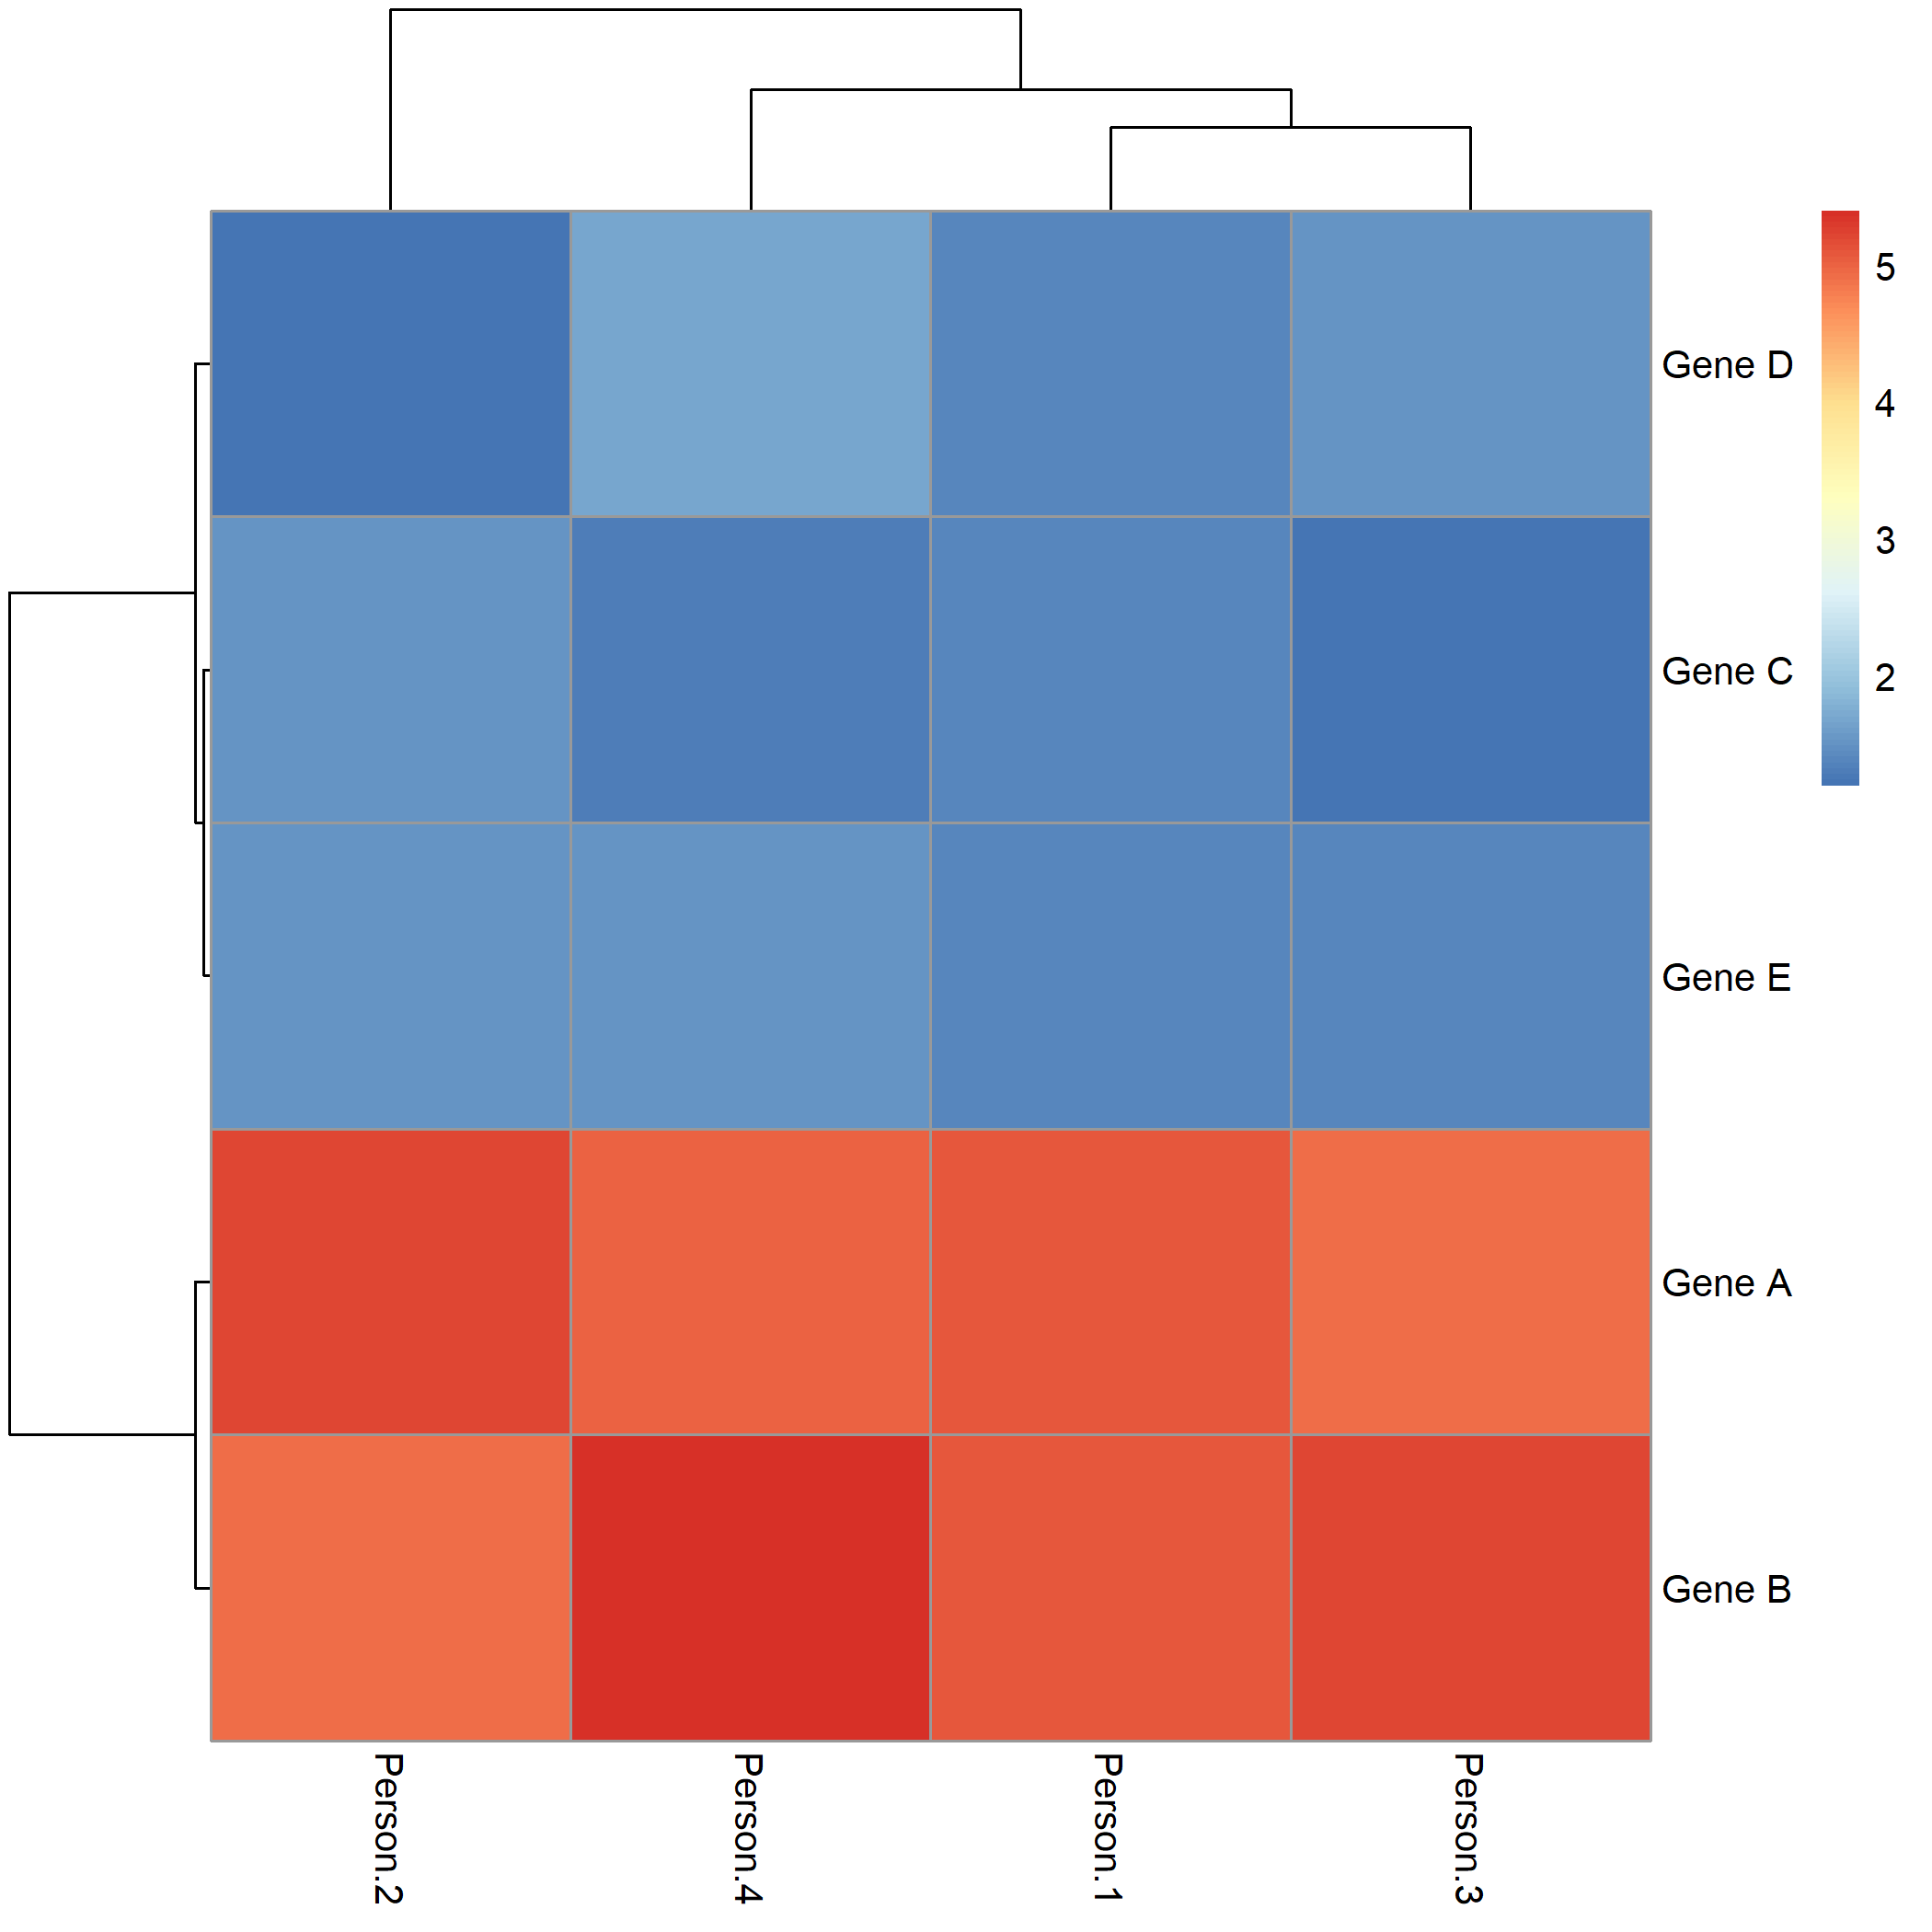
\includegraphics[scale=0.55]{Images/Examples/example_expression_data.png}
		\caption{Heatmap of expression data in table \ref{table:example_gene_expression_data} showing the clusters based upon magnitude of expression.}
		\label{fig:example_expression_data}
	\end{figure}
	One can see that genes A and C have similar patters in variation across the people, as do genes B and D. Gene E is not consistent with any other gene here. However, as this relative variation is of interest rather than the magnitude of expression, one can see that standardising the data is required. If one were to cluster the data as represented in table \ref{table:example_gene_expression_data}, one would place genes A and B in one cluster and genes C, D and E in another as their absolute expression levels are similar (as can be seen in figure \ref{fig:example_expression_data}). However, if the expression level of each gene is standardised as per section \ref{sec:standardisation}, the data is then as represented in table \ref{table:example_standardised_gene_expression_data}. As the data are now on the same scale the characteristic that will determine a clustering is the variation of expression across people. As we want genes with similar patterns of variation (i.e. that are co-expressed) this enables us to cluster under our objective of defining gene sets. In this case genes A and C are one cluster, genes B and D another with gene E in a cluster alone, as can be seen in figure \ref{fig:example_standardised_expression_data}. As this is the type of data we wish to cluster across, we therefore most standardise our expression data before clustering can be implemented.

	\begin{table}[] 
	\centering
	\begin{tabular}{c|cccc} 
	Genes 	& Person 1	& Person 2	& Person 3	& Person 4	\\ 
	\hline
	A 		& 0.39		& 1.16 		& -1.16		& -0.39		\\
	B 		& -0.24		& -1.20		& 0.24		& 1.20		\\
	C 		& 0.39		& 1.16		& -1.16		& -0.39		\\
	D 		& -0.24		& -1.20		& 0.24		& 1.20		\\
	E 		& -0.87		& 0.87		& -0.87		& 0.87		
	\end{tabular}
	\caption{Example standardised gene expression data.}
	\label{table:example_standardised_gene_expression_data}
	\end{table}
	
	\begin{figure}[h]
	\centering
		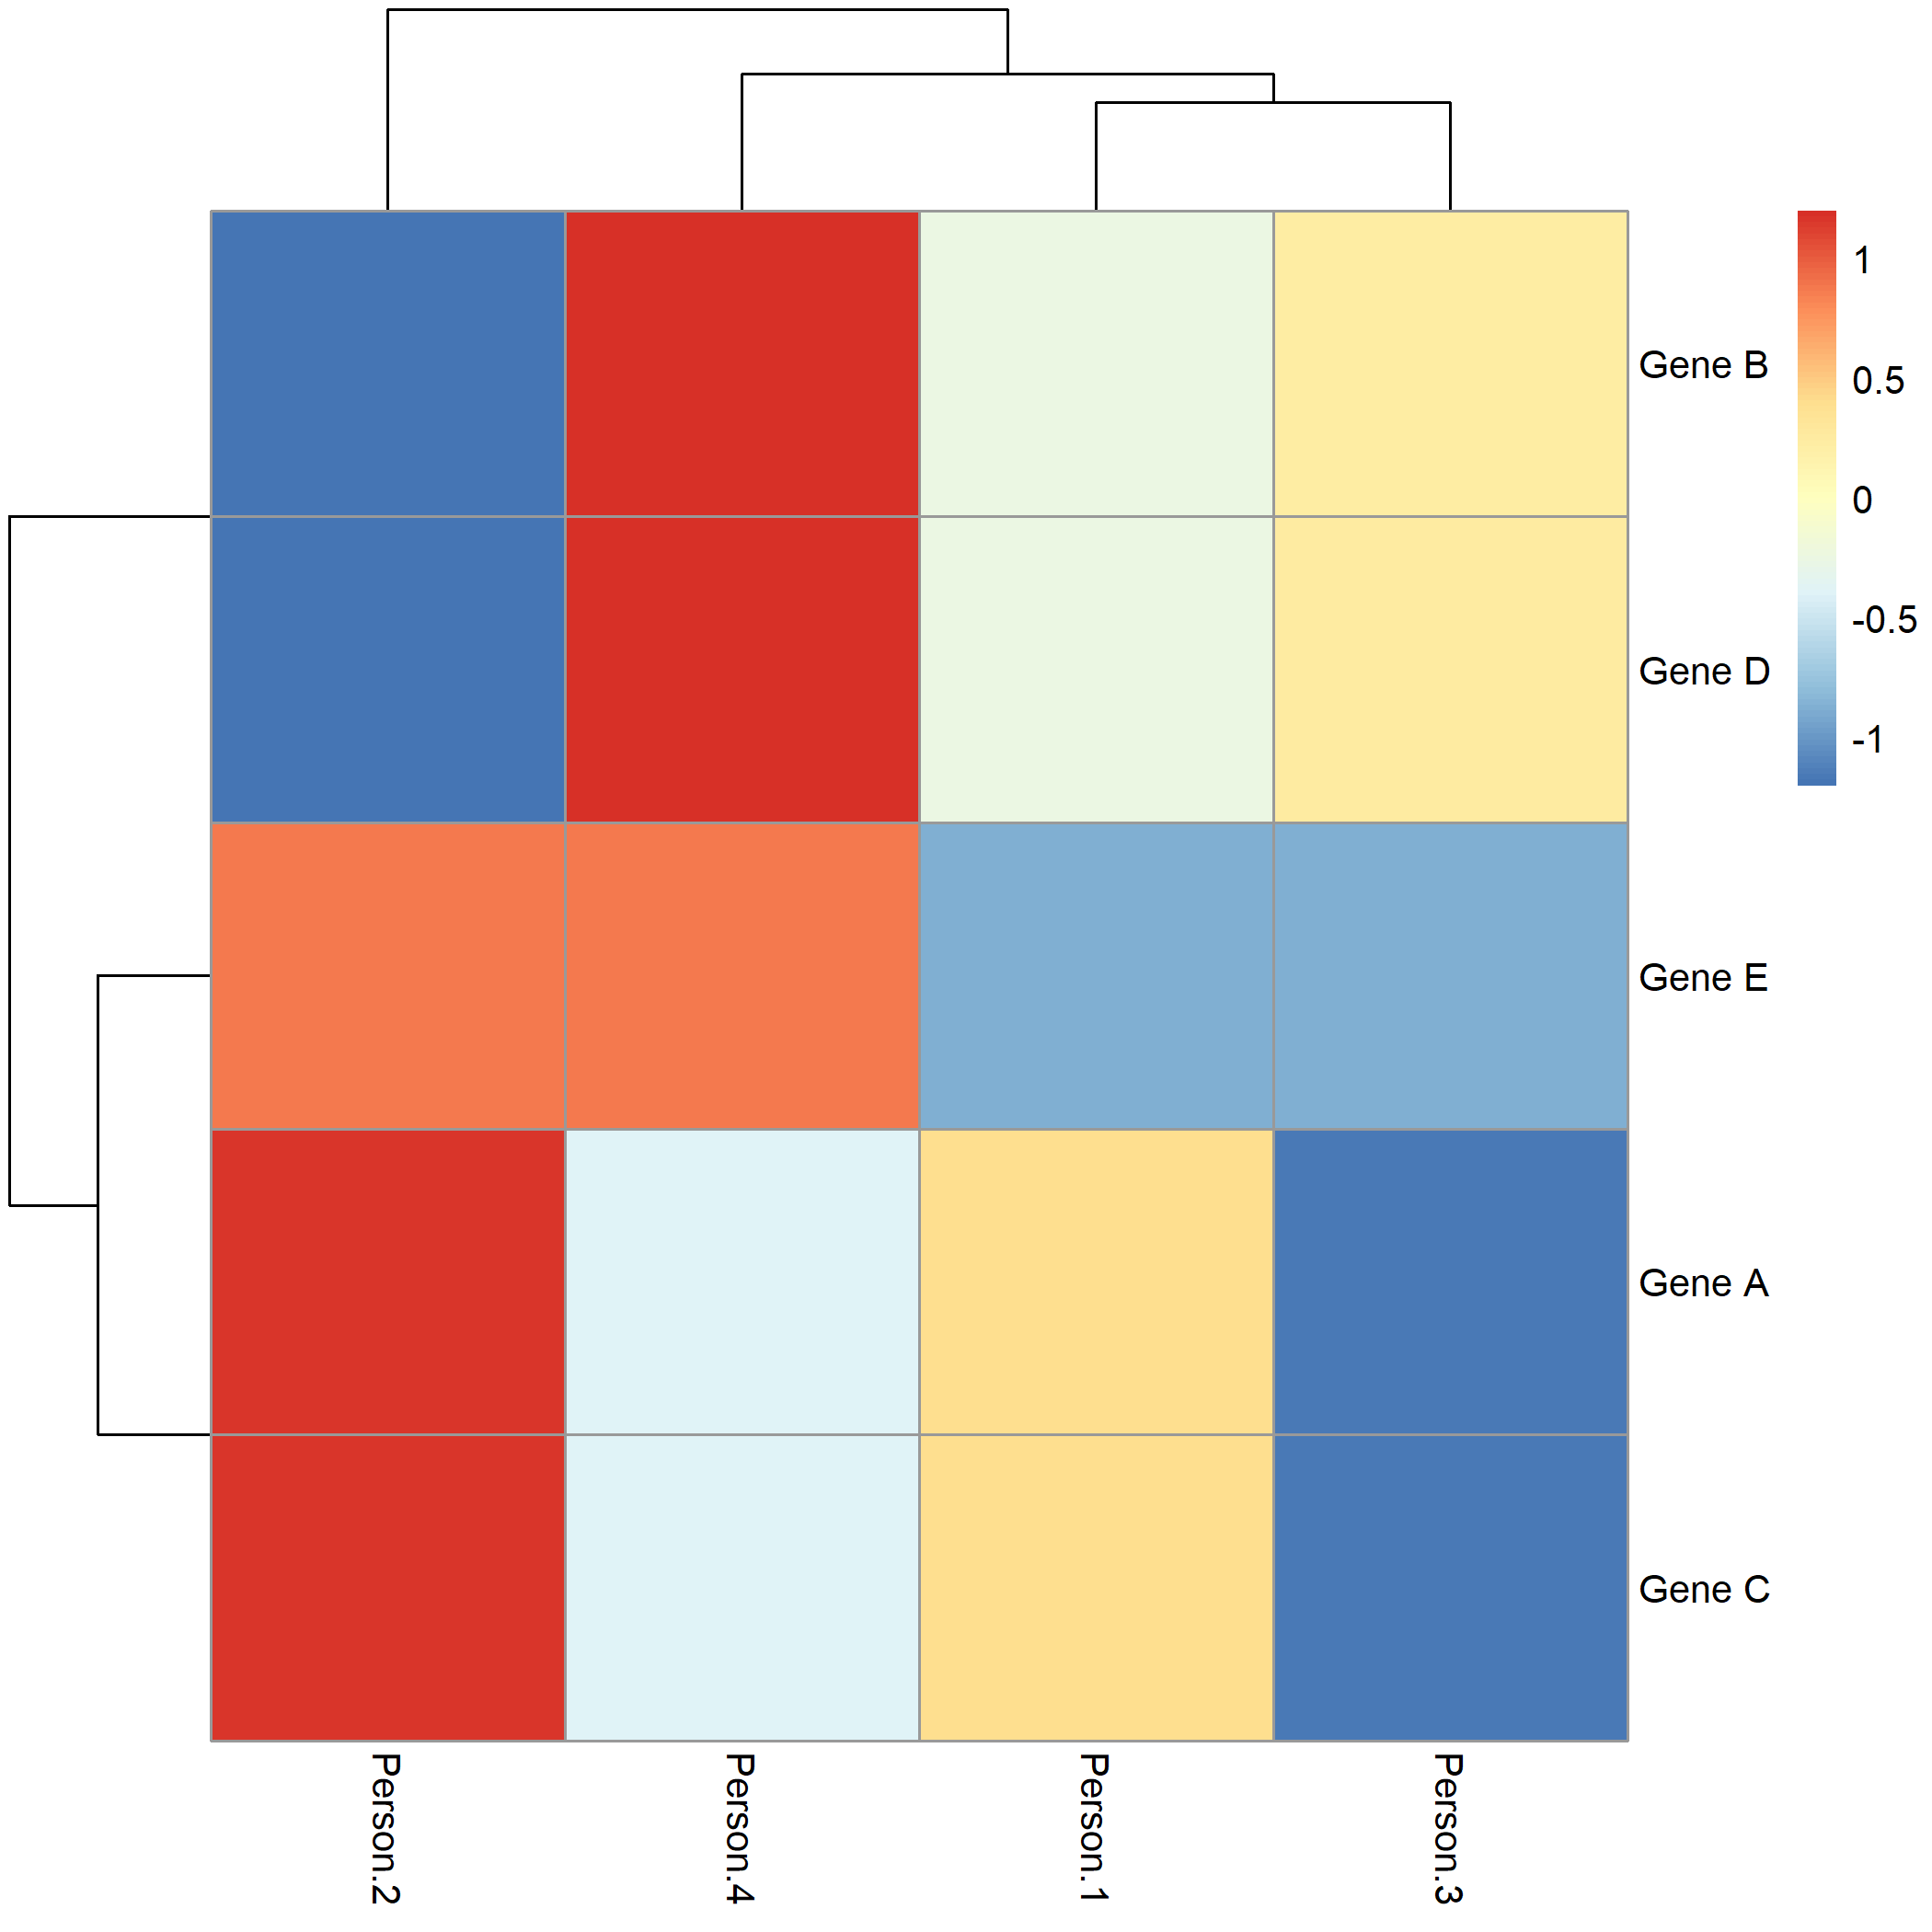
\includegraphics[scale=0.55]{Images/Examples/example_standardised_expression_data.png}
		\caption{Heatmap of expression data in table \ref{table:example_standardised_gene_expression_data} showing the clusters based upon variation of expression across people.}
		\label{fig:example_standardised_expression_data}
	\end{figure}
		
%	\subsection{The importance of gene sets}
%	If we can cluster genes together it is possible that we can find deeper biological interpretation, understanding the context of the gene products and what they interact with. This can offer some insight into the connection between the gene and the expressed phenotype. Furthermore, \citet{NicaExpressionquantitativetrait2013} recommend investigating groups of cis-eQTL affecting a gene network that when perturbed results in a disease state. They claim this is far higher powered than the classical approach. This claim is supported by the findings of \citet{VosaUnravelingpolygenicarchitecture2018} who found that associations between \emph{polygenic risk scores} and gene expression (this association is referred to as ``expression quantitative trait score'' (eQTS) in \cite{VosaUnravelingpolygenicarchitecture2018}) contained the most biological information about disease in a comparison of cis-eQTL, trans-EQTL and eQTS. This finding is not unique to this paper \cite{DudbridgePowerPredictiveAccuracy2013}\cite{WrayResearchReviewPolygenic2014}. More generally, gene set enrichment analysis (GSEA) \cite{SubramanianGenesetenrichment2005a}\cite{MooneyGenesetanalysis2015} relies upon pre-defined gene sets. This method determines if gene sets have statistically significant, concordant differences between phenotypes and offers biological interpretation of the sets. Thus well-defined gene sets are required for informative, interpretable analysis of genomic information.
	
	
%	\subsection{Existing databases}
%	There exist many databases of gene sets \cite{AshburnerGeneOntologytool2000a}\cite{KanehisaNewapproachunderstanding2019}\cite{SzklarczykSTRINGv11protein2019}. The Molecular Signature Database \cite{SubramanianGenesetenrichment2005a} (MSigDB) is one of the most popular resources for GSEA and encompasses many different gene sets defined under different criteria or generated from different resources. However, none of these definitions of a ``set'' incorporate tissue specific information. 
%	(such as the Gene Ontology (GO) Resource \cite{AshburnerGeneOntologytool2000a}, the Kyoto Encyclopedia of Genes and Genomes (KEGG) \cite{KanehisaNewapproachunderstanding2019}, the Molecular Signatures Database (MSigDB) \cite{SubramanianGenesetenrichment2005a} or the STRING protein-protein interaction (PPI) database \cite{SzklarczykSTRINGv11protein2019})
	
	

%	\subsection{Variance stabilisation}
	

	\subsection{Data}
	We use the gene expression data from Correlated Expression and Disease Association Research (CEDAR) cohort \cite{TheInternationalIBDGeneticsConsortiumIBDriskloci2018}. This data is avialable in a processed form \href{http://139.165.108.18/srv/genmol/permanent/1be6993fe41c12a051c9244d67c91da2be49e5dd26a6cd79f442bc006971e2ef/crohn-index.html}{online}. This consists of 9 .csv files, one for each tissue / cell type present of normalised gene expression data for 323 individuals. These are healthy individuals of European descent; the cohort consists of 182 women and 141 men with an average age of 56 years (but ranging from 19 to 86). None of the individuals are suffering from any autoimmune or inflammatory disease and were not taking corticosteroids or non-steroid anti-inflammatory drugs (with the exception of aspirin). 
	
	With regards to tissue types, samples from six circulating immune cells types (followed in brackets by the abbreviation for the associated dataset):
	\begin{itemize}
		\item CD4+ T lymphocytes (CD4);
		\item CD8+ T lymphocytes (CD8);
		\item CD14+ monocytes (CD14);
		\item CD15+ granulocytes (CD15);
		\item CD19+ B lymphocytes (CD19); and 
		\item platelets (PLA).
	\end{itemize}
	Data from intestinal biopsies are also present, with samples taken from three distinct locations:
	\begin{itemize}
		\item the illeum (IL);
		\item the rectum (RE); and
		\item the colon (TR).
	\end{itemize} 
	Not every individual is present in every dataset. However, as we are clustering genes this should not present a problem.
	
	Whole genome expression data were generated using HT-12 Expression Beadchips following the instructions of the manufacturer (Illumina). There are 18,524 probes present between the 9 datasets.
	
%	\begin{figure}[h]
	\begin{sidewaysfigure}
		\centering
		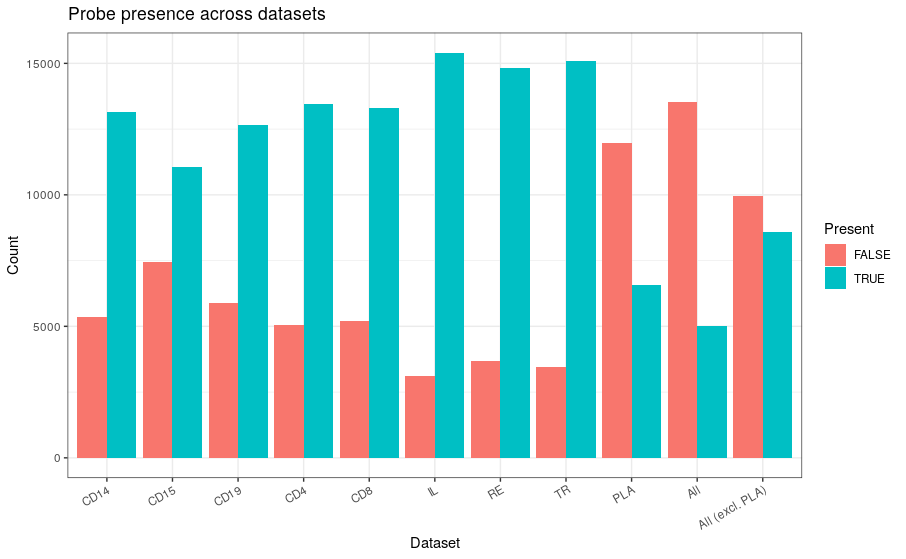
\includegraphics[scale=0.9 ]{Images/Data_inspection/probe_presence_across_datasets.png}
		\caption{Probe presence across datasets. Under ``All'' we have the number of probes present in every dataset, under ``All (excl. PLA)'' we have the number of probes present in every dataset bar PLA. Note how there is greater missingness in the PLA dataset in comparison to the others.}
		\label{fig:probe_presence_across_datasets}
	\end{sidewaysfigure}
%	\end{figure}
	
	The fluorescence intensities were $\log_2$ transformed and Robust Spline Normalized with Lumi38.
	
	It should be noted that there are differing degrees of missingness between the datasets (for instance the platelets dataset has 6,564 probes present in comparison to an average of 12,838 probes present per dataset, see figure \ref{fig:probe_presence_across_datasets}).
	
	Due to this and the exponential increase in computational cost for each additional dataset, we use only the 8 most informative datasets, dropping PLA from our analysis. From a biological perspective we also expect PLA to be the least rich as platelets have no nucleus citeWRIGHT and therefore any gene expression is an artefact from before they differentiated into platelets. 

%	Individuals were genotyped for more than 700,000 SNPs using Illumina's Human OmniExpress BeadChips, an iScan system and the Genome Studio software following the guidelines of the manufacturer. Variants were elimanted with call rate $\leq 0.95$, deviating from Hardy-Weinberg equilibrium $(p \leq 0.95)$, or which were monomorphic.
%	
%	Using the real genotypes of 629,570 quality-controlled autosomal SNPs as anchors, Sangar Imputation Services were used with the UK10K $+$ 1000 Genomes Phase 3 Haplotype panels to impute genotypes at autosomal variants in the population. The following were removed from the dataset indels, SNPs :
%	\begin{itemize}
%		\item with minor allele frequency (MAF) $\leq 0.05$;
%		\item deviating from Hardy-Weinberg equilibrium $(p \leq 10^{-3}$); and
%		\item with low imputation quality (INFO $\leq 0.4$).
%	\end{itemize}
%	This left $6,019,462$ high quality SNPs for eQTL analysis.
%	
%	Whole genome expression data were generated using HT-12 Expression Beadchips following the instructions of the manufacturer (Illumina). Technical outliers were removed using controls recommended by Illumina and the Lumi package
%	
%	We kept $29,464/47,323$ autosomal probes (corresponding to 19,731 genes) mapped by Re-Annotator39 to a single gene body with $\leq 2$ mismatches and not spanning known variants with MAF$>0.05$. Within cell types, we only considered probes (i.e., “usable” probes) with detection $p-value \leq 0.05$ in $\geq 25\%$ of the samples. Fluorescence intensities were $\log_2$ transformed and Robust Spline Normalized (RSN) with Lumi38.
	
	
	\section{Methods}
	We first show via simulated data that MDI can cluster appropriately and that the consensus clustering does produce similar results to a converged single run.
	
	We then simulate data where individual chains of MDI will struggle to converge and possibly will not converge in finite time. We show that consensus clustering explores a wider space than any individual chain and appears to describe something similar to the space described by the union of the chains.
	
	Finally we apply consensus clustering to 1,000 probes for 8 datasets from the CEDAR dataset. An initial set of probes are chosen based on the members of 3 KEGG pathways:
	
	\begin{enumerate} \label{list:kegg_pathways}
		\item Inositol phosphate metabolism (a broad biological pathway);
		\item NOD-like receptor signaling pathway (a specific biological pathway with known involvement in IBD \cite{CarneiroNodlikeproteinsinflammation2008}\cite{GarrettHomeostasisInflammationIntestine2010}); and
		\item Inflammatory bowel disease (IBD) (a pathological pathway).
	\end{enumerate}
	The union of these sets corresponds to 169 unique genes (or 287 probes as the mapping from the space of probes to that of genes is non-injective) that are present in the CEDAR dataset. The remaining probes are randomly selected from the total possible space (18,524 probes) less those corresponding to these genes (leaving 18,287 possible candidate probes). We then expect that the genes from the sets mentioned above (list \ref{list:kegg_pathways}) should cluster together. We use this as a test of our final clustering.
	
	\subsection{CEDAR data pipeline}
	For the CEDAR data, we follow this pipeline to prepare the data for clustering:
	\begin{enumerate} \label{list:methods}
		\item Transpose the data to have rows associated with gene probes and columns associated with individuals;
		\item Remove NAs either imputing values using the minimum expressed value (as missingness is not random) or if above a threshold of missingness removing the column;
		\item Standardise the data;
%		\item Apply variance stabilisation \cite{huber_variance_2002} to normalise the gene expression data;
%		\item Inspect the data by PCA and remove outlier individuals for each dataset in each gene set;
		\item To apply MDI we require that each dataset have the same row names in the same order, so we re-arrange our datasets to have common order of probes;
		\item For probes entirely missing from a given dataset we generate expression from a standard normal distribution for each probe. Then these probes are expressed as noise in the dataset and any clustering imposed upon them should be due to information about these probes present in other datasets; and
		\item Apply MDI \cite{MasonMDIGPUacceleratingintegrative2016a}.
	\end{enumerate}
	
	\section{Results}
%	\subsection{Simulations}
	\subsection{Case 1: Proof of consensus}
	Generated data based on data from original MDI paper with some additional noisy clusters that MDI succeeds with.
	
%	\begin{figure}[h]
		\begin{sidewaysfigure}
			\centering
			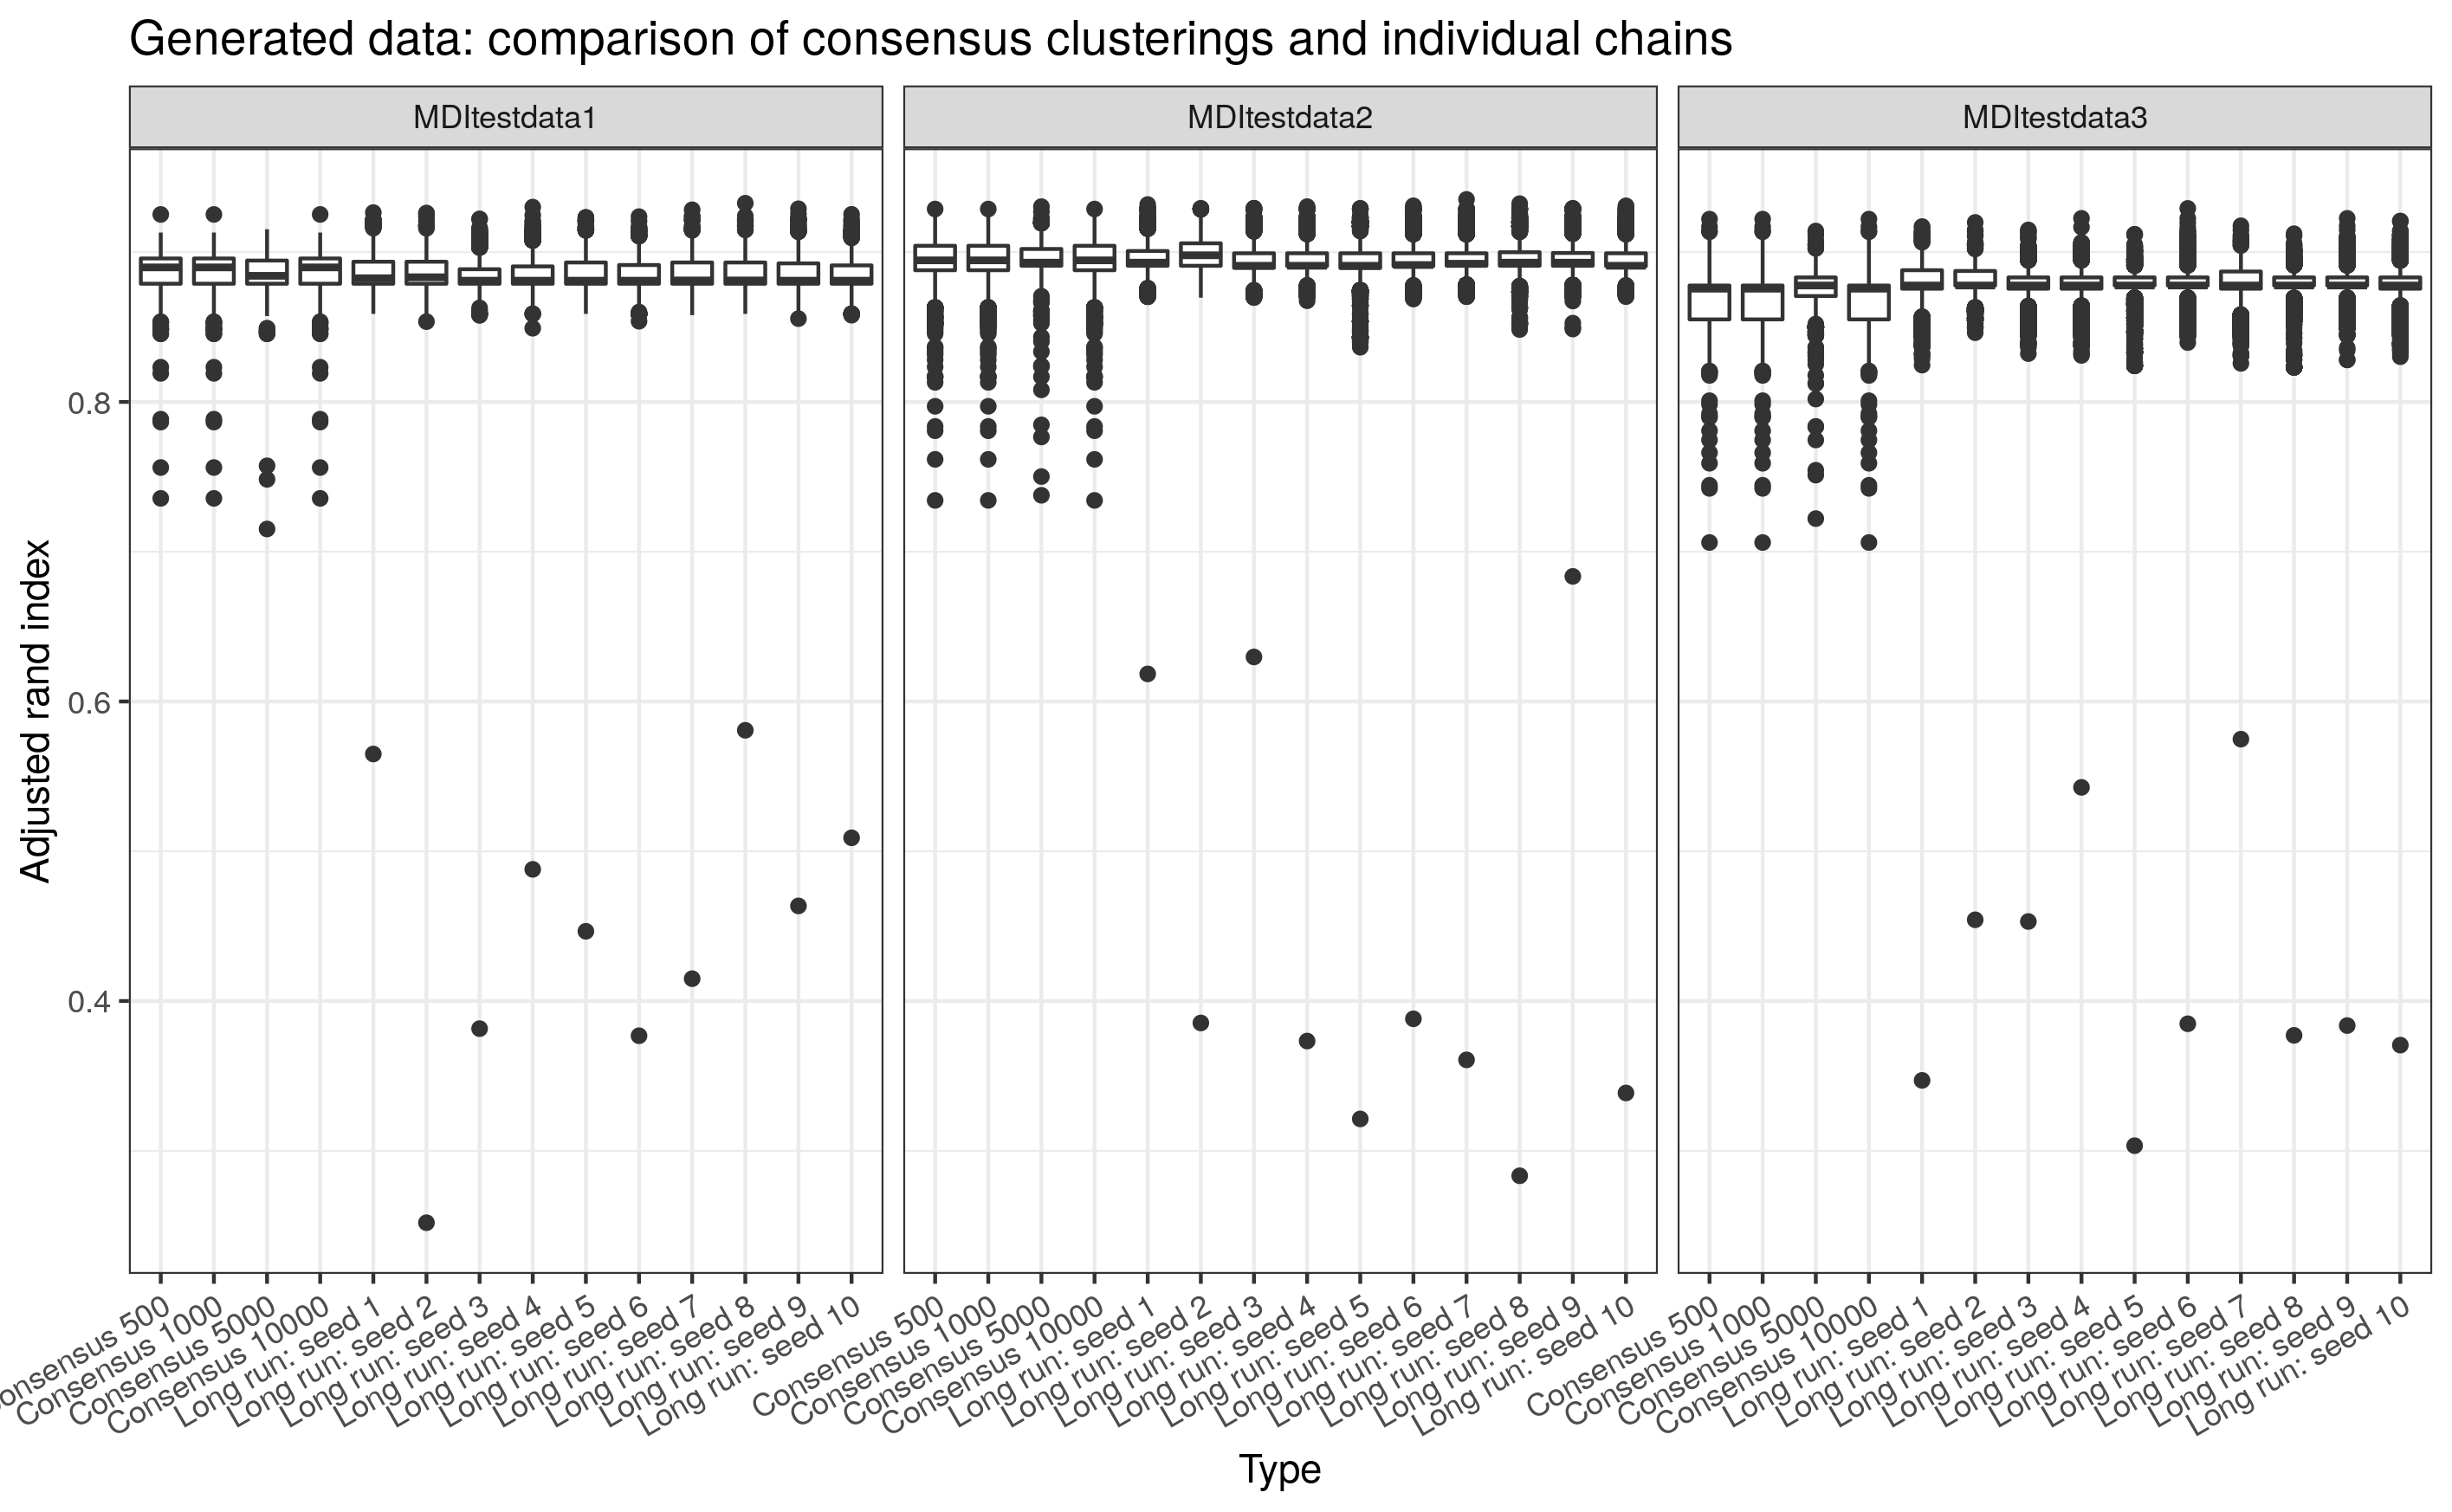
\includegraphics[scale=0.9]{Images/Gen_data/Case_1/box_plot_ari_true_clustering.png}
			\caption{Box plots for distribution of adjusted rand index between the clustering at each iteration to the true clustering for different lengths of consensus clustering and different initialisation of long chains.}
			\label{fig:gen_data_case_1_boxplot}
		\end{sidewaysfigure}
		%	\end{figure}
		
		\begin{figure}[h]
			\centering
			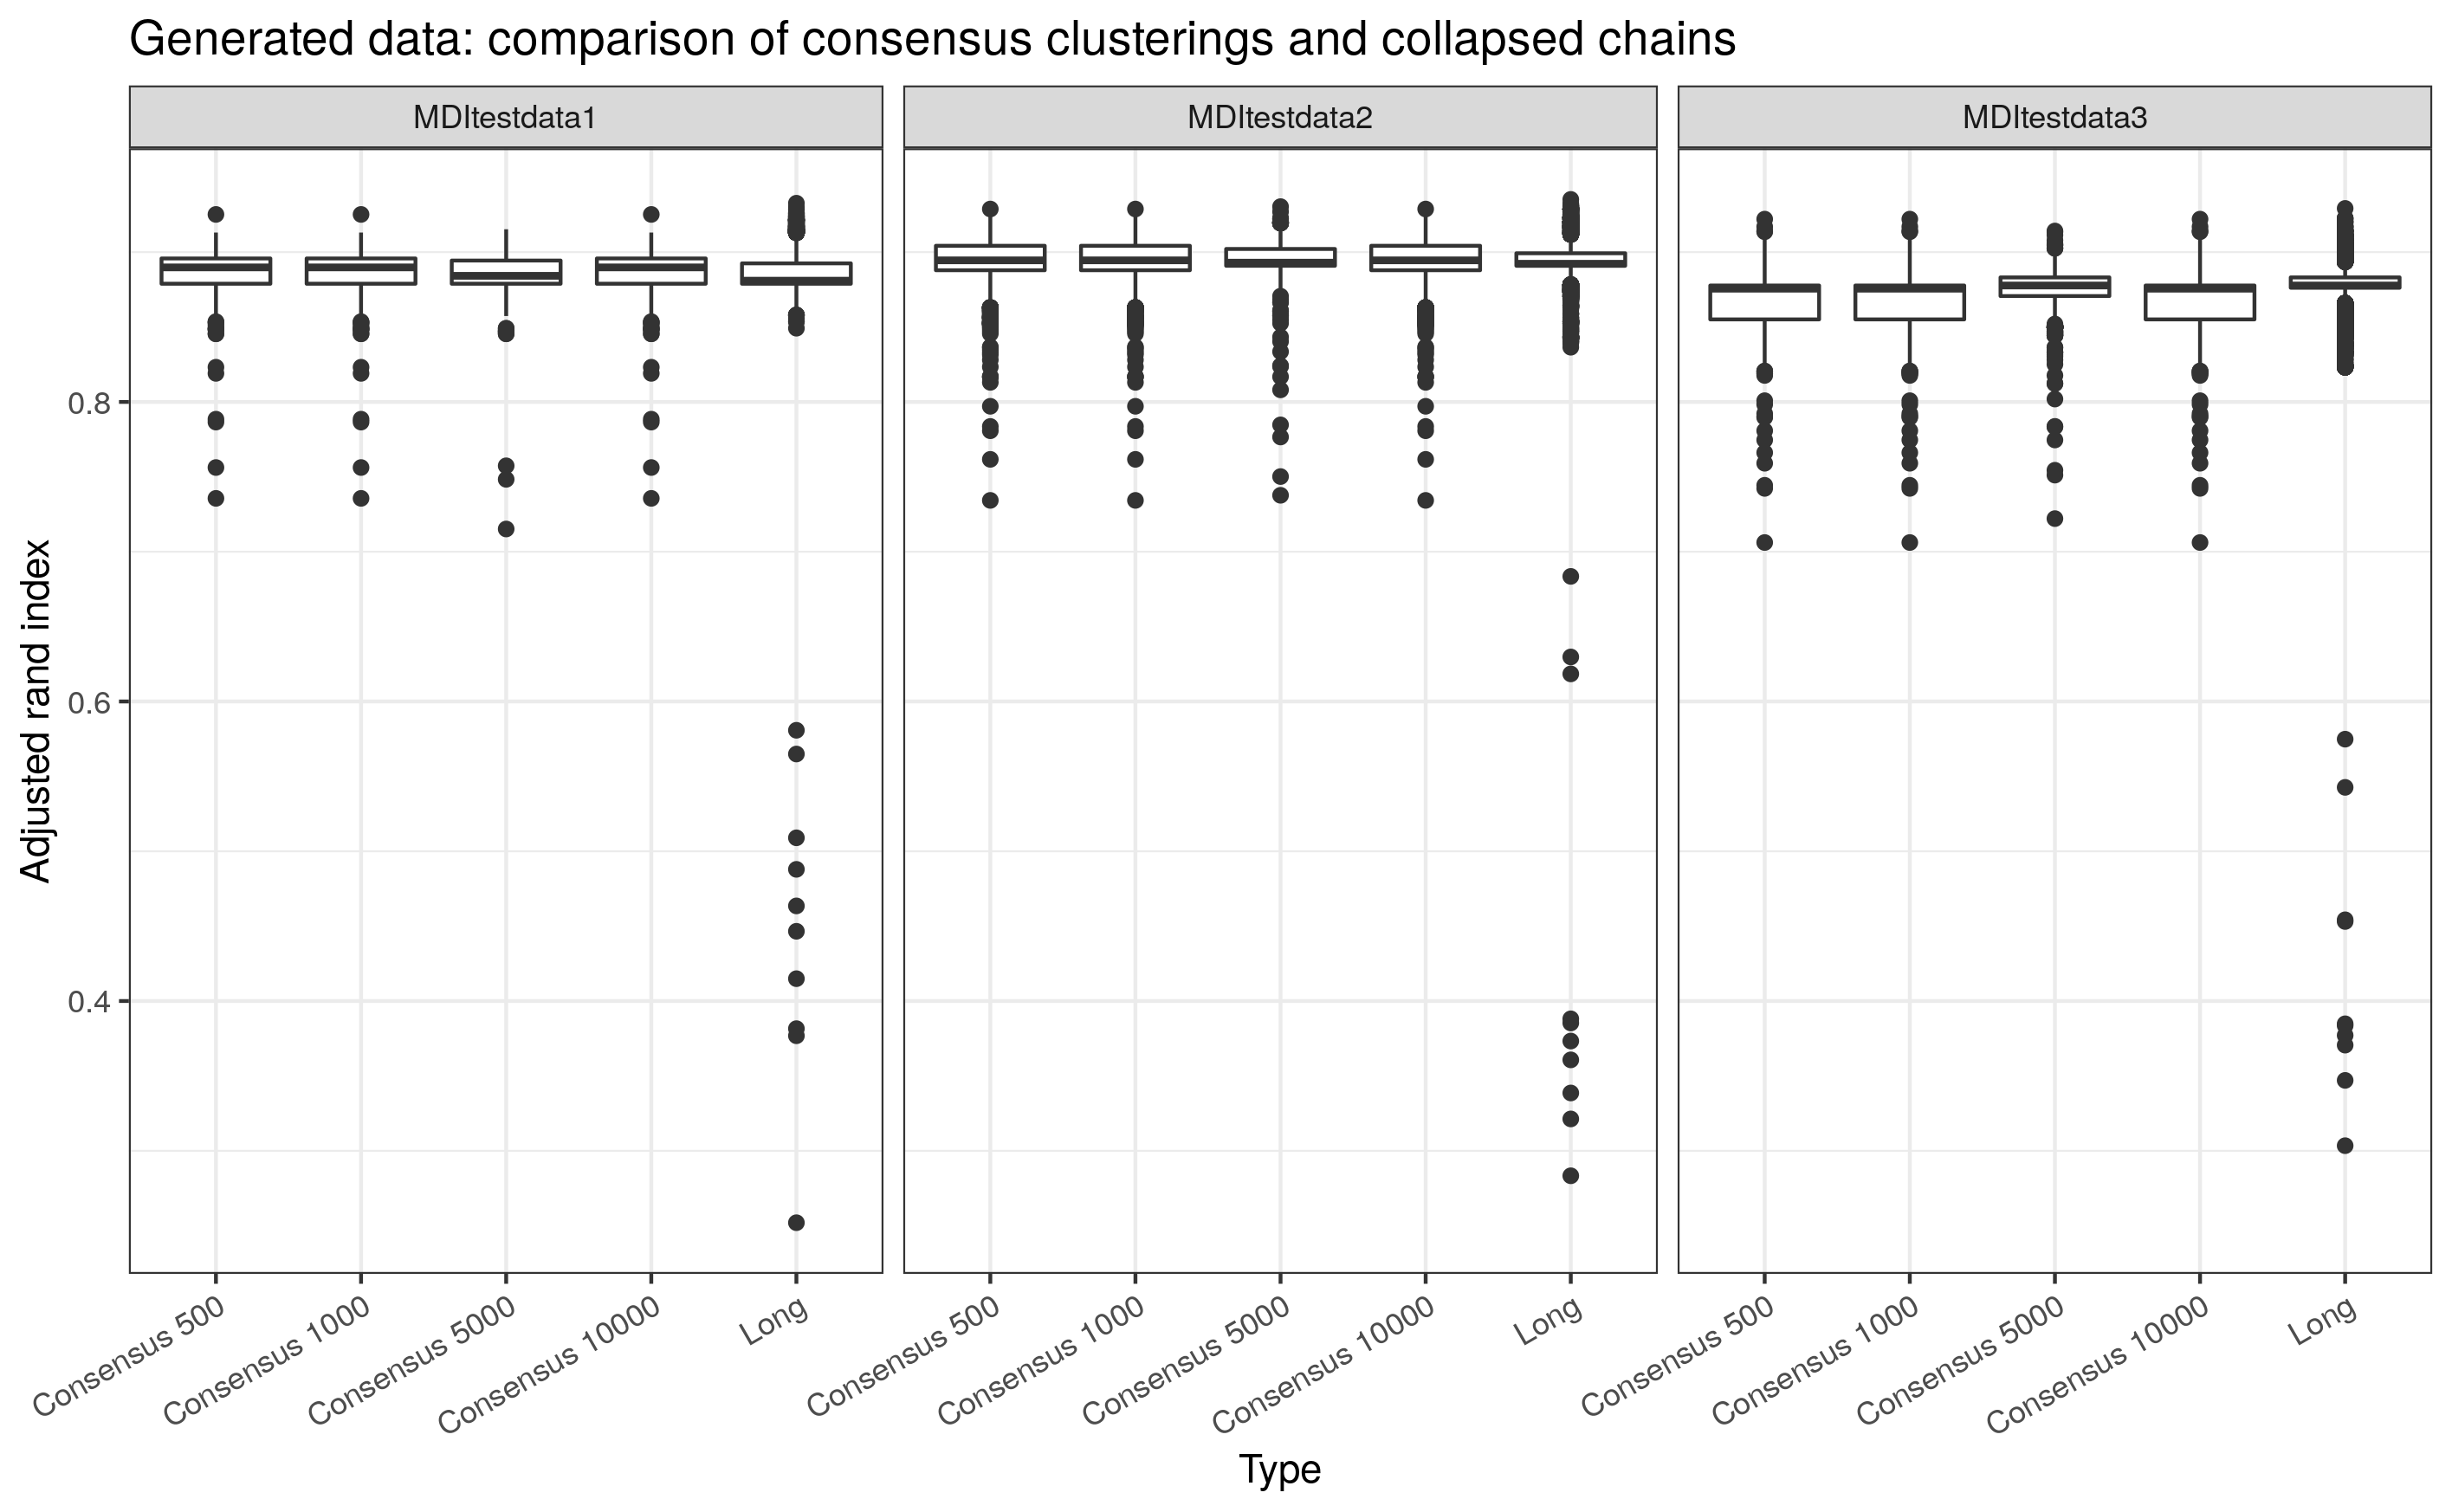
\includegraphics[scale=0.65]{Images/Gen_data/Case_1/box_plot_ari_true_clustering_collapsed_long.png}
			\caption{Box plots for distribution of adjusted rand index between the clustering at each iteration to the true clustering for different lengths of consensus clustering and the collapsed long chains.}
			\label{fig:gen_data_case_1_collapsed_boxplot}
		\end{figure}
	
	\subsection{Case 2: Overcoming multiple modes}
	Generated data that MDI struggles with.
	
%	\begin{figure}[h]
		\begin{sidewaysfigure}
		\centering
		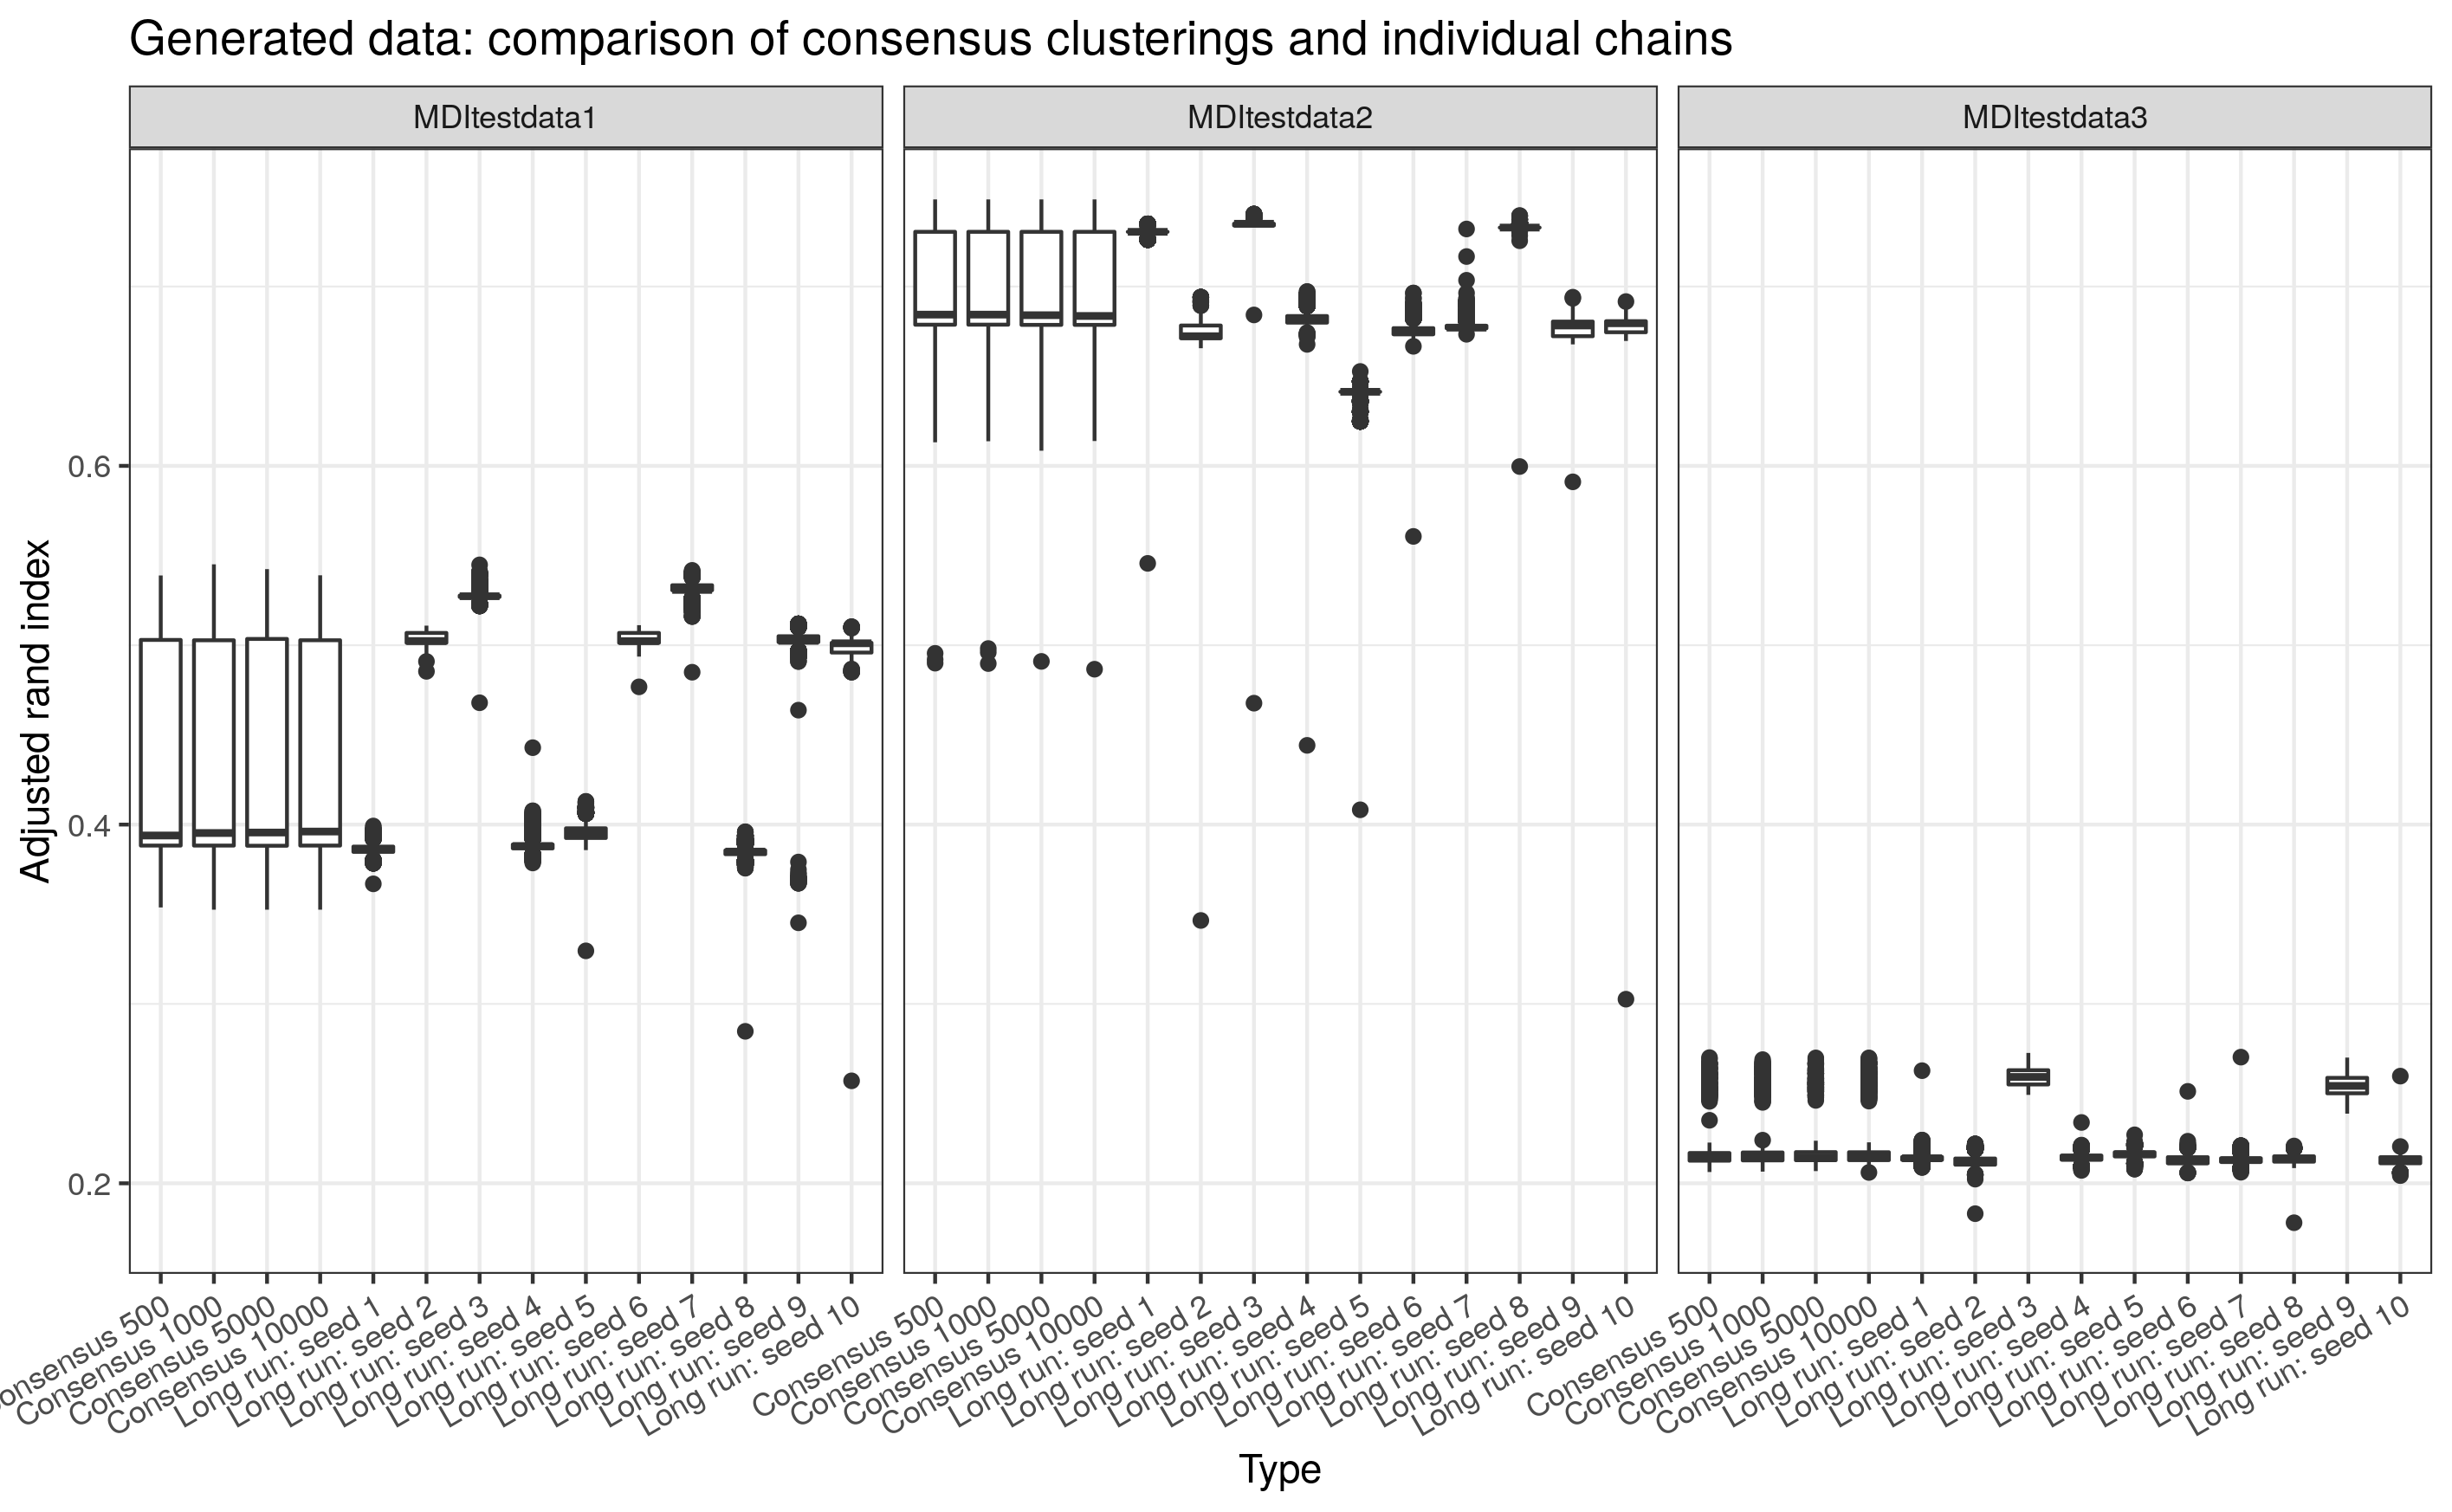
\includegraphics[scale=0.9]{Images/Gen_data/Case_2/box_plot_ari_true_clustering.png}
		\caption{Box plots for distribution of adjusted rand index between the clustering at each iteration to the true clustering for different lengths of consensus clustering and different initialisation of long chains.}
		\label{fig:gen_data_case_2_boxplot}
	\end{sidewaysfigure}
%	\end{figure}

	\begin{figure}[h]
		\centering
		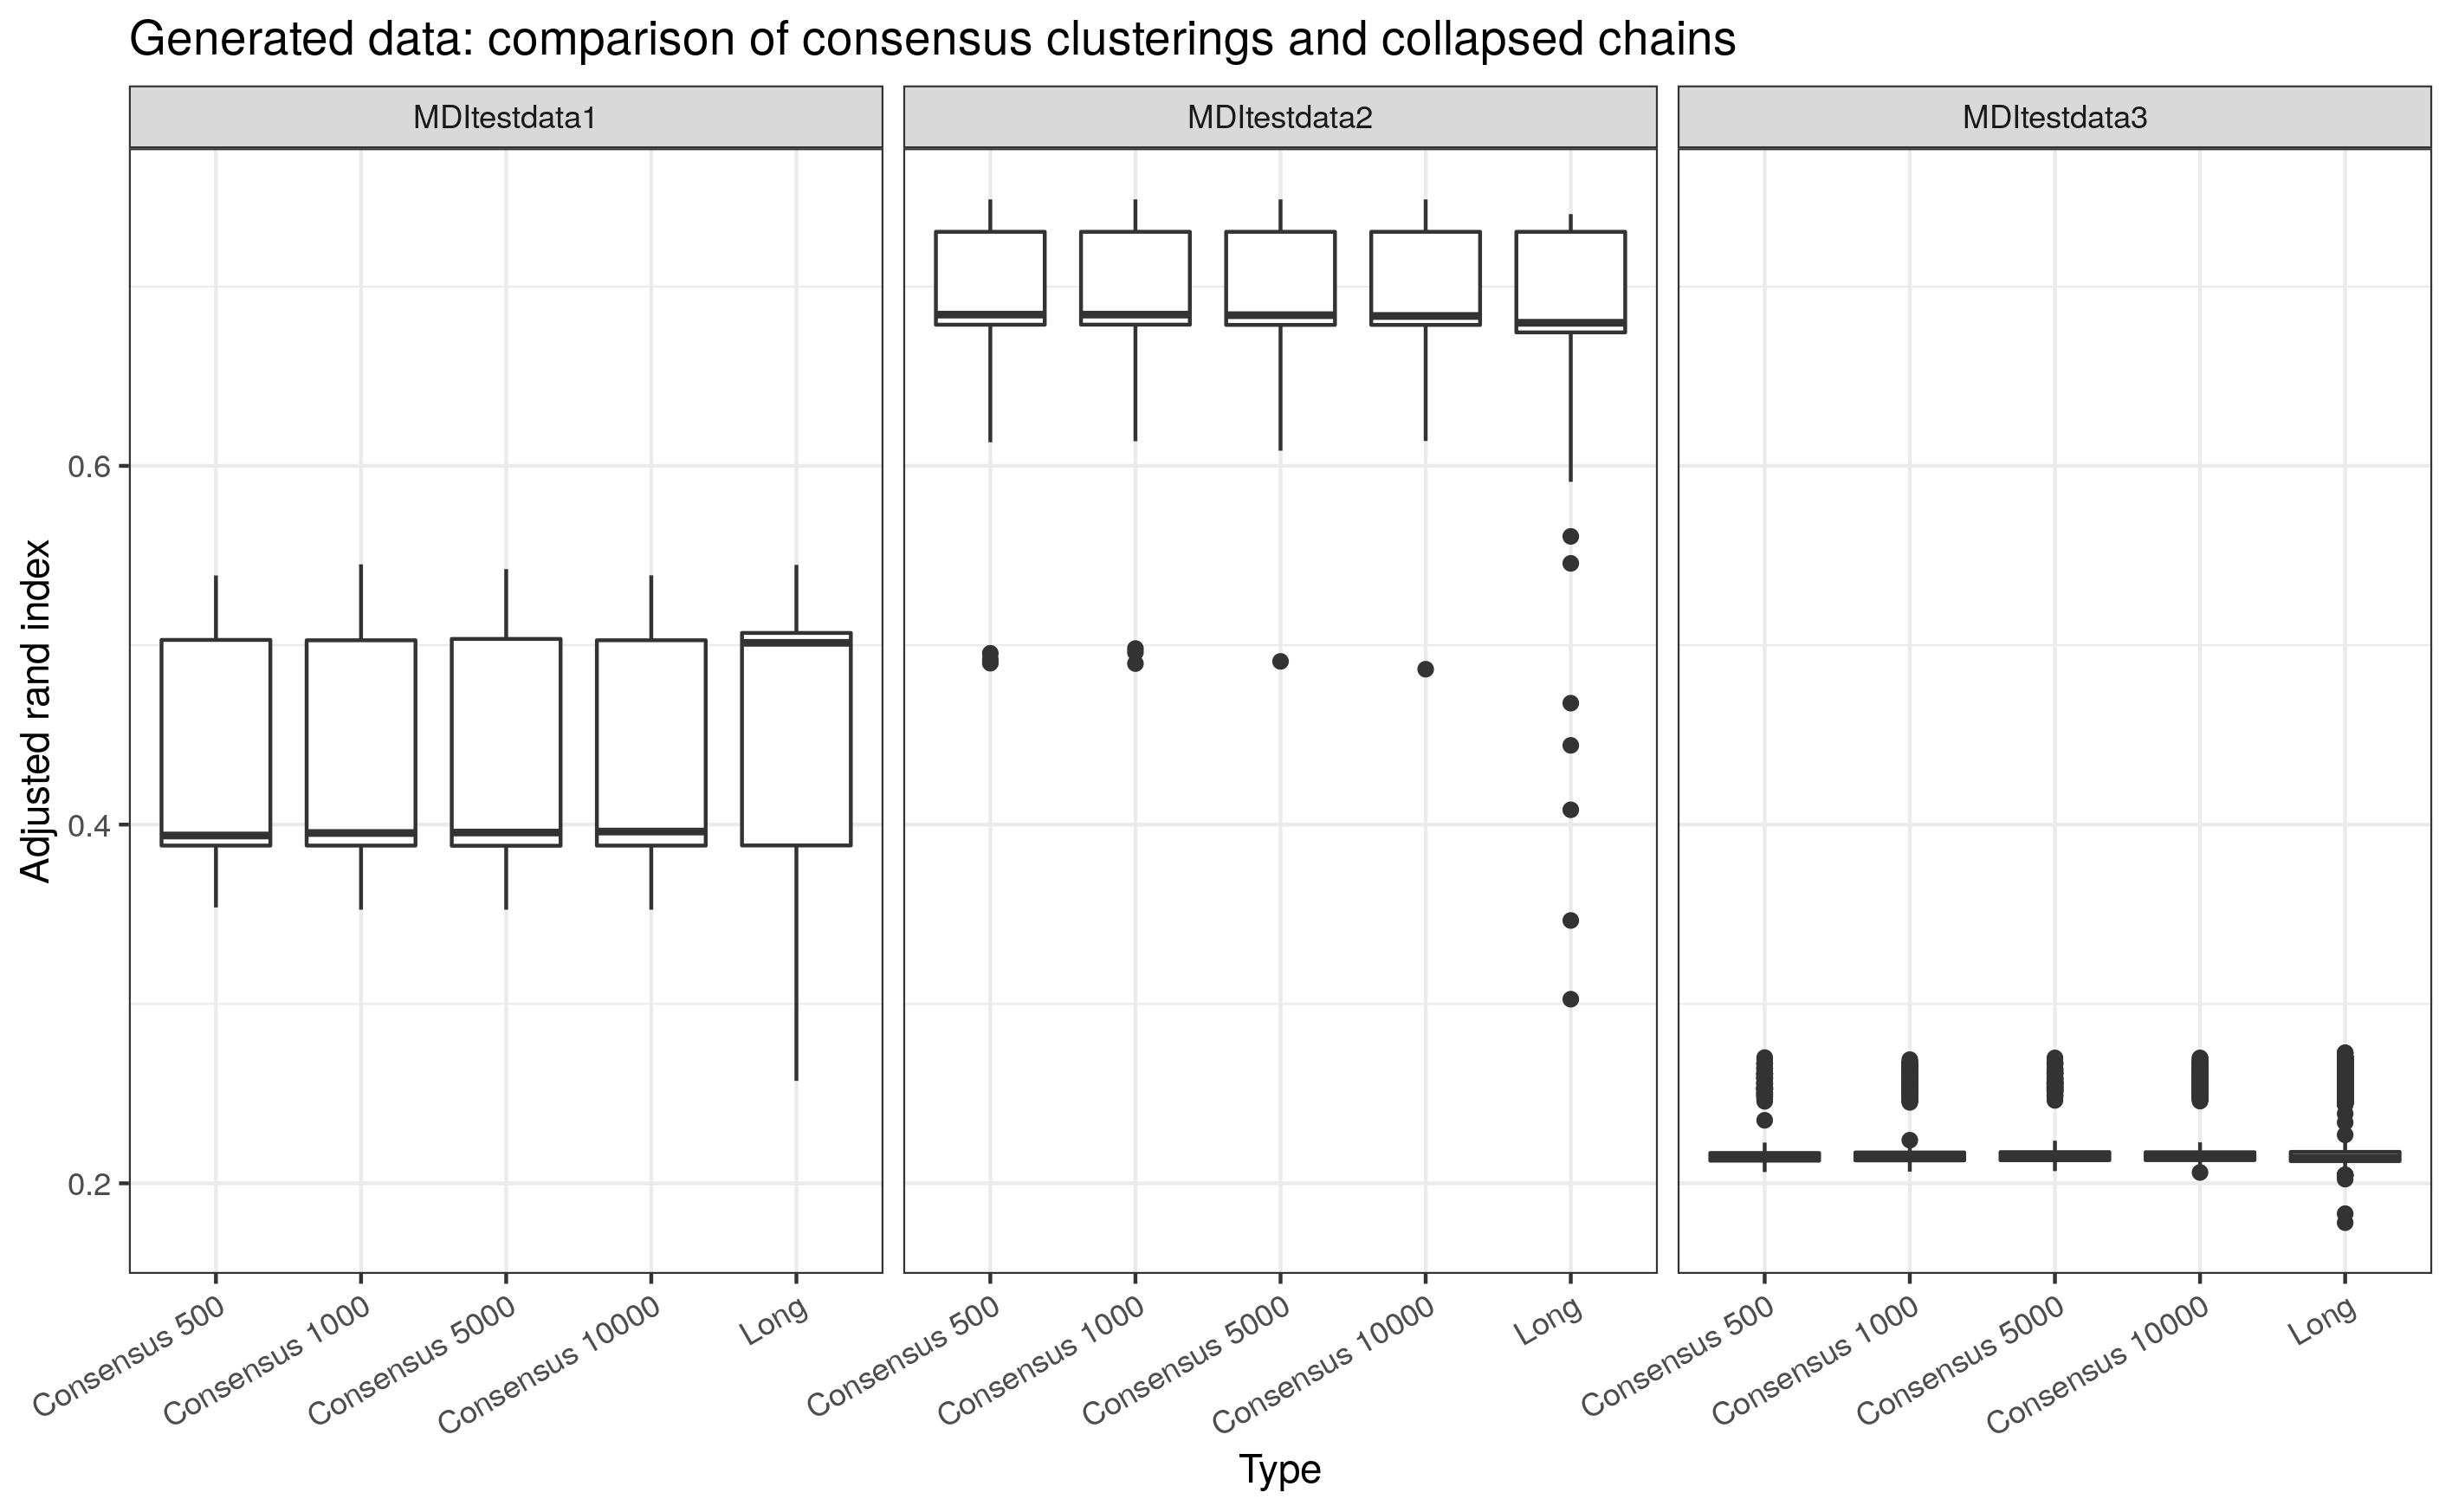
\includegraphics[scale=0.65]{Images/Gen_data/Case_2/box_plot_ari_true_clustering_collapsed_long.png}
		\caption{Box plots for distribution of adjusted rand index between the clustering at each iteration to the true clustering for different lengths of consensus clustering and the collapsed long chains.}
		\label{fig:gen_data_case_2_collapsed_boxplot}
	\end{figure}

	\begin{figure}[h]
		\centering
		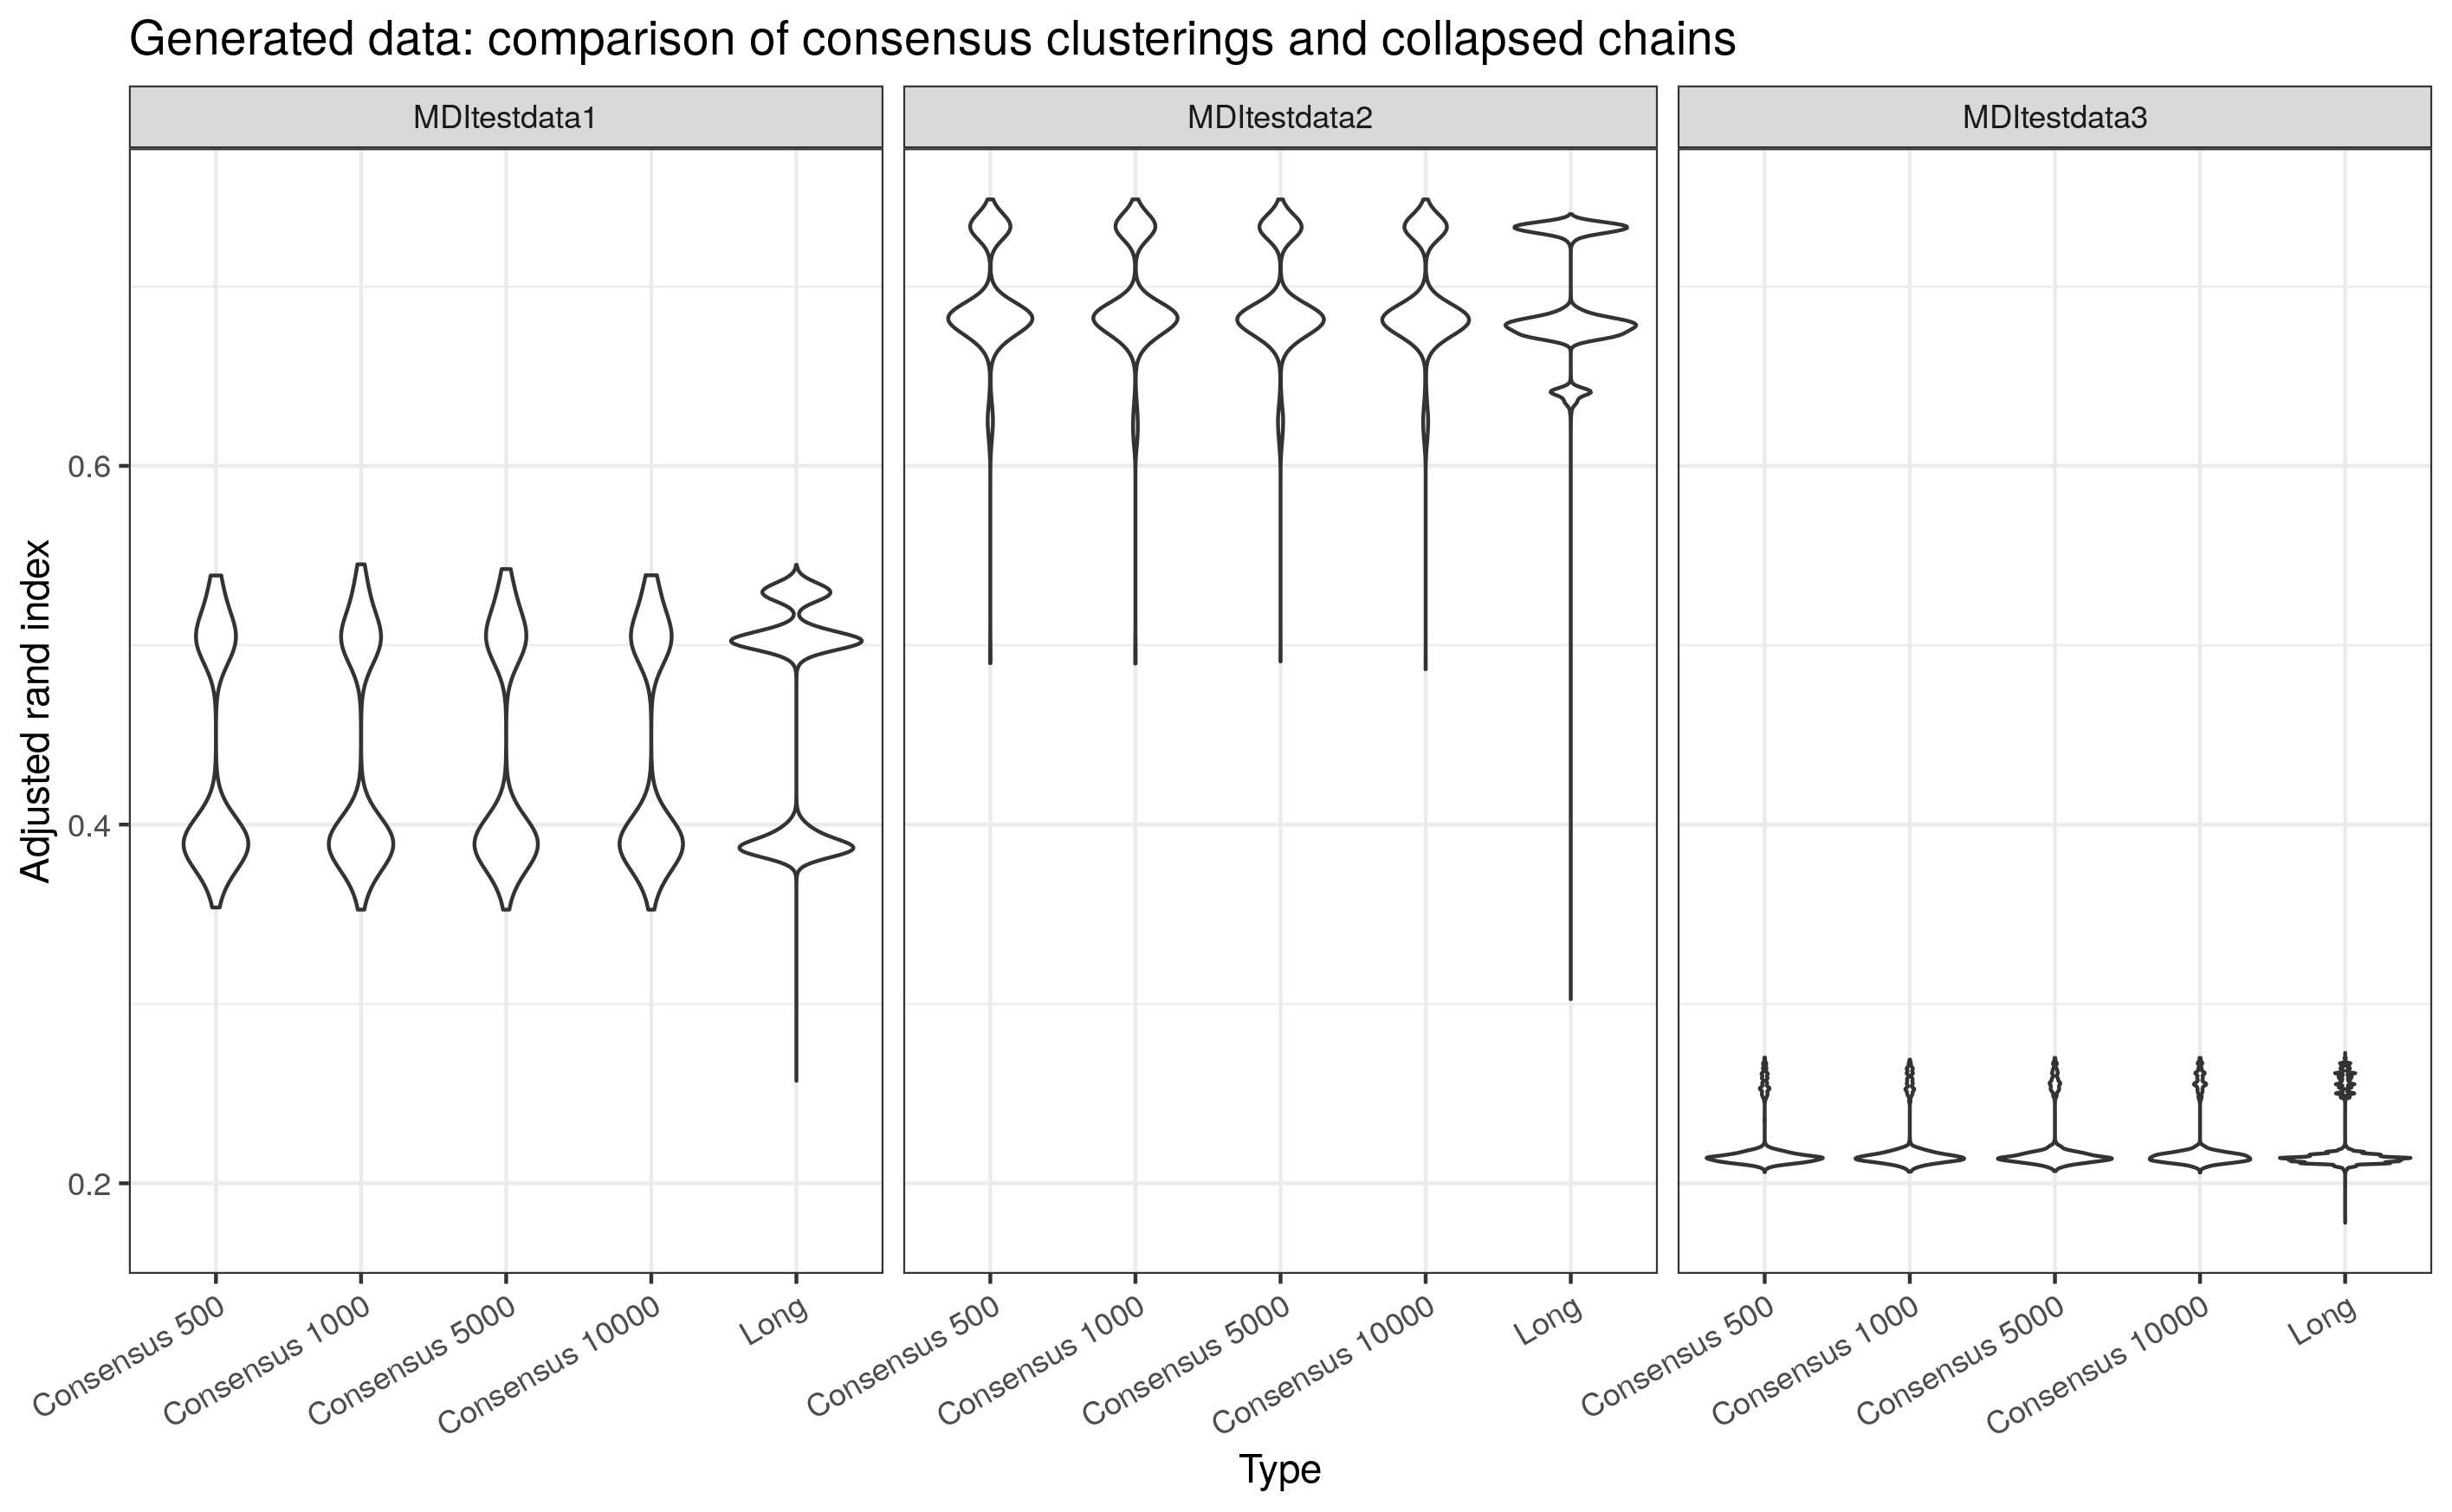
\includegraphics[scale=0.65]{Images/Gen_data/Case_2/violin_plot_ari_true_clustering_collapsed_long.png}
		\caption{Violoin plots for distribution of adjusted rand index between the clustering at each iteration to the true clustering for different lengths of consensus clustering and the collapsed long chains. We can see that the consensus clustering approximates the modes described across chains quite well.}
		\label{fig:gen_data_case_2_collapsed_violin_plot}
	\end{figure}

	\subsection{Case 3: CEDAR data}
	Actual data.
	
	\section{Conclusion}
	We conclude, and finish dispute.
	
	
	
%	\newpage
%	\begin{table}[]
%		\centering
%		\begin{tabular}{l|CCCCCC}
%			Case   & \alpha_1 & \alpha_2 & \alpha_3 & \phi_{12}   & \phi_{13}   & \phi_{23} \\
%			\hline
%			Case 1 & 0.951            & 0.912            & 0.705            & 0.534   & 0.893   & 0.705   \\
%			Case 1 & 0.804            & 0.787            & 0.516            & 0.563   & 0.605   & 0.787   \\
%			Case 1 & 0.627            & 0.784            & 0.592            & 0.534   & 0.789   & 0.985   \\
%			Case 1 & 0.870             & 0.912            & 0.534            & 0.686   & 0.951   & 0.743   \\
%			Case 1 & 0.516            & 0.534            & 0.985            & 0.686   & 0.705   & 0.951   \\
%			Case 1 & 0.893            & 0.534            & 0.951            & 0.985   & 0.705   & 0.743   \\
%			Case 1 & 0.790	& 0.787            & 0.867            & 0.705   & 0.992   & 0.888   \\
%			Case 1 & 0.563            & 0.534            & 0.592            & 0.789   & 0.572   & 0.534   \\
%			Case 1 & 0.516            & 0.784            & 0.985            & 0.627   & 0.985   & 0.893   \\
%			Case 1 & 0.743            & 0.892            & 0.892            & 0.743   & 0.787   & 0.572  
%		\end{tabular}
%		\caption{Test statistic from Geweke diagnostic of convergence for each parameter for case 1 chains.}
%	\label{table:geweke_case_1}
%	\end{table}
%
%		\begin{table}[]
%		\centering
%		\begin{tabular}{l|CCCCCC}
%			Case   & \alpha_1 & \alpha_2 & \alpha_3 & \phi_{12}   & \phi_{13}   & \phi_{23} \\
%			\hline
%			Case 2 & 0.867            & 0.787            & 0.951            & 0.821   & 0.87    & 0.789   \\
%			Case 2 & 0.787            & 0.516            & 0.847            & 0.743   & 0.686   & 0.951   \\
%			Case 2 & 0.787            & 0.627            & 0.516            & 0.870    & 0.87    & 0.897   \\
%			Case 2 & 0.705            & 0.789            & 0.795            & 0.592   & 0.985   & 0.605   \\
%			Case 2 & 0.787            & 0.870             & 0.893            & 0.516   & 0.787   & 0.985   \\
%			Case 2 & 0.867            & 0.795            & 0.87             & 0.784   & 0.893   & 0.870    \\
%			Case 2 & 0.534            & 0.534            & 0.516            & 0.870    & 0.705   & 0.563   \\
%			Case 2 & 0.605            & 0.969            & 0.784            & 0.897   & 0.534   & 0.516   \\
%			Case 2 & 0.743            & 0.705            & 0.592            & 0.827   & 0.892   & 0.883   \\
%			Case 2 & 0.563            & 0.534            & 0.893            & 0.563   & 0.592   & 0.787  
%		\end{tabular}
%	\caption{Test statistic from Geweke diagnostic of convergence for each parameter for case 2 chains.}
%	\label{table:geweke_case_2}
%	\end{table}
%
%
%\begin{table}[]
%	\begin{tabular}{l|CCCCCC}
%		Case   & \alpha_1 & \alpha_2 & \alpha_3 & \phi_{12}   & \phi_{13}   & \phi_{23} \\
%		\hline
%		Case 1 & 0.157            & -0.256           & -1.129           & -1.905  & -0.325  & 1.098   \\
%		Case 1 & -0.66            & -0.819           & 2.288            & 1.587   & -1.368  & 0.792   \\
%		Case 1 & 1.307            & -0.888           & 1.499            & -1.766  & 0.732   & 0.042   \\
%		Case 1 & -0.484           & -0.263           & 1.779            & -1.22   & 0.152   & 0.984   \\
%		Case 1 & -2.115           & -1.837           & 0.062            & 1.212   & -1.104  & -0.164  \\
%		Case 1 & -0.331           & 1.748            & 0.195            & 0.031   & 1.148   & 0.984   \\
%		Case 1 & -0.705           & 0.762            & 0.549            & 1.166   & -0.011  & -0.411  \\
%		Case 1 & -1.607           & 1.977            & 1.478            & 0.722   & -1.538  & 1.725   \\
%		Case 1 & -2.139           & -0.88            & 0.029            & 1.3     & -0.086  & -0.353  \\
%		Case 1 & 1.026            & 0.378            & -0.382           & 0.974   & -0.779  & 1.548   \\
%		Case 2 & -0.542           & -0.768           & 0.161            & -0.632  & -0.458  & 0.74    \\
%		Case 2 & 0.781            & 2.296            & 0.587            & 0.966   & -1.204  & 0.189   \\
%		Case 2 & -0.775           & -1.302           & 2.52             & 0.482   & -0.477  & -0.292  \\
%		Case 2 & -1.076           & -0.717           & -0.68            & 1.43    & 0.078   & -1.377  \\
%		Case 2 & -0.768           & -0.514           & -0.333           & -2.164  & 0.792   & -0.06   \\
%		Case 2 & 0.535            & -0.685           & 0.45             & -0.884  & 0.336   & -0.464  \\
%		Case 2 & -1.99            & 1.768            & -2.202           & 0.457   & 1.088   & -1.602  \\
%		Case 2 & -1.392           & 0.12             & 0.902            & -0.303  & 1.816   & -2.591  \\
%		Case 2 & -0.993           & 1.133            & 1.434            & 0.617   & -0.377  & 0.427   \\
%		Case 2 & -1.588           & 1.798            & 0.316            & 1.589   & -1.429  & -0.85  
%	\end{tabular}
%\end{table}
%
%
%\begin{table}[]
%	\begin{tabular}{l|CCCCCC}
%		Case   & \alpha_1 & \alpha_2 & \alpha_3 & \phi_{12}   & \phi_{13}   & \phi_{23} \\
%		\hline
%		Case 1 & 0.157            & -0.256           & -1.129           & -1.905  & -0.325  & 1.098   \\
%		Case 1 & -0.66            & -0.819           & 2.288            & 1.587   & -1.368  & 0.792   \\
%		Case 1 & 1.307            & -0.888           & 1.499            & -1.766  & 0.732   & 0.042   \\
%		Case 1 & -0.484           & -0.263           & 1.779            & -1.22   & 0.152   & 0.984   \\
%		Case 1 & -2.115           & -1.837           & 0.062            & 1.212   & -1.104  & -0.164  \\
%		Case 1 & -0.331           & 1.748            & 0.195            & 0.031   & 1.148   & 0.984   \\
%		Case 1 & -0.705           & 0.762            & 0.549            & 1.166   & -0.011  & -0.411  \\
%		Case 1 & -1.607           & 1.977            & 1.478            & 0.722   & -1.538  & 1.725   \\
%		Case 1 & -2.139           & -0.88            & 0.029            & 1.3     & -0.086  & -0.353  \\
%		Case 1 & 1.026            & 0.378            & -0.382           & 0.974   & -0.779  & 1.548  
%	\end{tabular}
%\end{table}
%
%
%\begin{table}[]
%	\begin{tabular}{l|CCCCCC}
%		Case   & \alpha_1 & \alpha_2 & \alpha_3 & \phi_{12}   & \phi_{13}   & \phi_{23} \\
%		\hline
%		Case 2 & -0.542           & -0.768           & 0.161            & -0.632  & -0.458  & 0.74    \\
%		Case 2 & 0.781            & 2.296            & 0.587            & 0.966   & -1.204  & 0.189   \\
%		Case 2 & -0.775           & -1.302           & 2.52             & 0.482   & -0.477  & -0.292  \\
%		Case 2 & -1.076           & -0.717           & -0.68            & 1.43    & 0.078   & -1.377  \\
%		Case 2 & -0.768           & -0.514           & -0.333           & -2.164  & 0.792   & -0.06   \\
%		Case 2 & 0.535            & -0.685           & 0.45             & -0.884  & 0.336   & -0.464  \\
%		Case 2 & -1.99            & 1.768            & -2.202           & 0.457   & 1.088   & -1.602  \\
%		Case 2 & -1.392           & 0.12             & 0.902            & -0.303  & 1.816   & -2.591  \\
%		Case 2 & -0.993           & 1.133            & 1.434            & 0.617   & -0.377  & 0.427   \\
%		Case 2 & -1.588           & 1.798            & 0.316            & 1.589   & -1.429  & -0.85  
%	\end{tabular}
%\end{table}



%	\section{Results}
%	
%	To check if the algorithm ran and as an initial exploration of the data, we implemented the steps described in \ref{list:methods} applying MDI to all 9 datasets. This was done twice - on the first occasion probes missing from a dataset or containing NAs were dropped (resulting in a total dataset of 4,964 probes in each dataset) and on the second occasion using an imputed value of 0 for missing probes (on this occasion we dropped probes that had NAs in some columns in all datasets reducing the dataset from 18,523 to 18,517 probes).
%	
%	The algorithm was capable of running for 10,000 iterations with a thinning factor of 25 over both these set of data.
%	
%	We used the modal clustering as the predicted clustering as the labels became fixed and did not vary for the majority of iterations. We did not use the clustering implied by the PSM as the clusters were very defined and thus the uncertainty captured by the PSM was not necessary for the predicted clustering. Furthermore, the computational cost of calculating the PSM, particularly for the larger dataset, was quite high (the PSM is a $n \times n$ matrix).
%	
%	MDI begins with 50 clusters (as an approximation of a Dirichlet process - note that we can change the number of clusters present). In the 9 datasets the number of occupied clusters stabilised around 10 (ranging from 8 - 13).
%	
%	We inspected the resulting clusters using the \emph{pheatmap} package \cite{KoldepheatmapPrettyHeatmaps2018} in R \cite{RCoreTeamLanguageEnvironmentStatistical2018}.
%	
%	\begin{figure}[h]
%	%	\centering
%		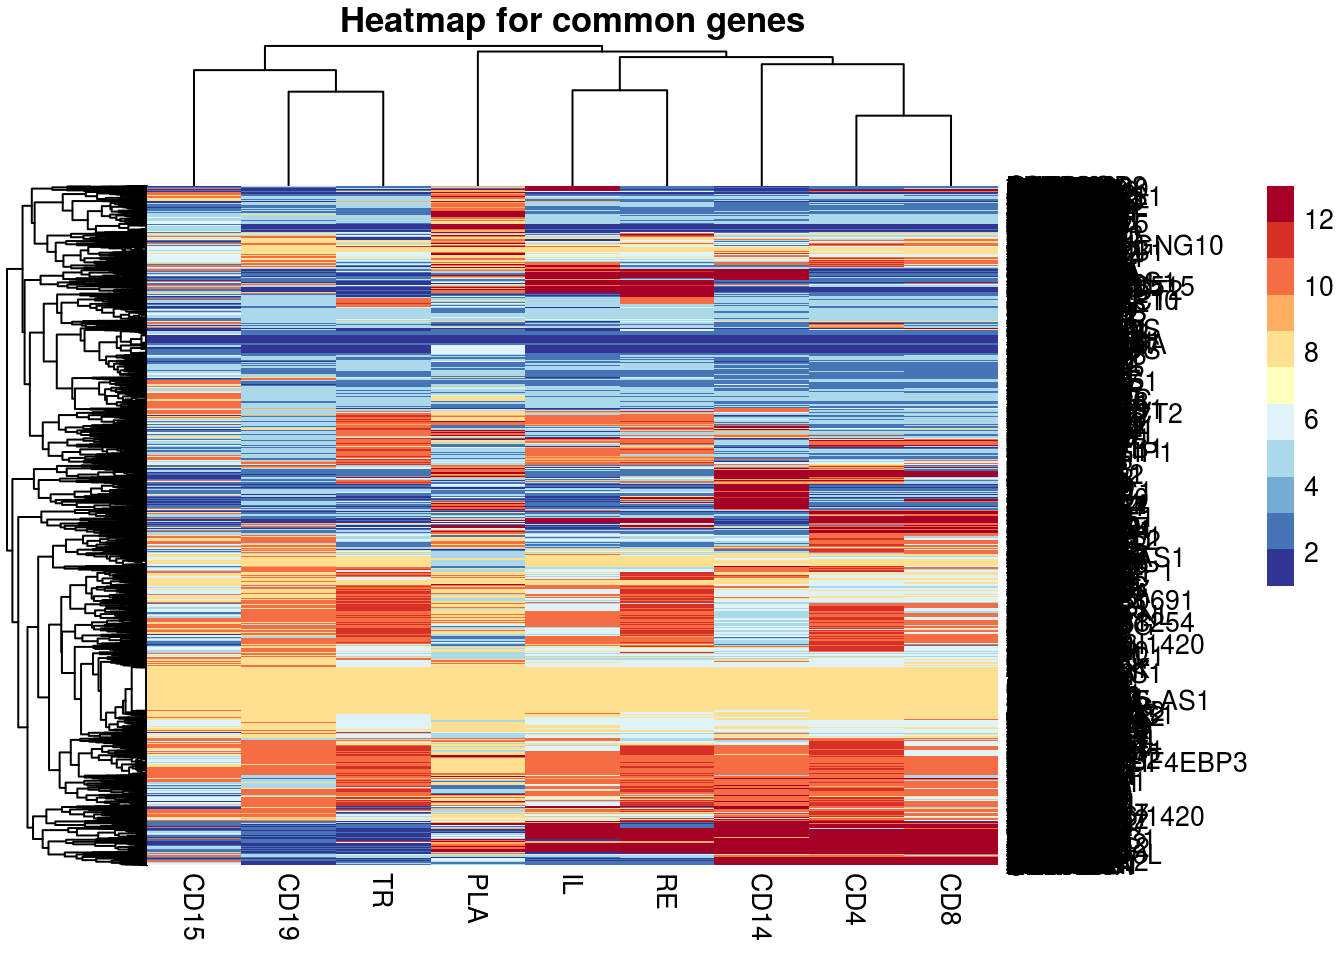
\includegraphics[scale=1.0]{Images/Initial_analysis/mdi_1_heatmap-1.png}
%		\caption{Predicted clusters for MDI applied to 9 datasets for common probes with datasets as columns and probes as rows.}
%		\label{fig:naive_mdi_reduced}
%	\end{figure}
%
%	We can see from figure \ref{fig:naive_mdi_reduced} that some genes cluster across all datasets (the beige band about 0.25 along the vertical axis). Between the combination of a visual inspect and the hierarchical clustering visible in the tree at the top of figure \ref{fig:naive_mdi_reduced} combined with the information in figure \ref{fig:naive_mdi_reduced_phi_heatmap}, one can see that the platelets behave significantly differently to the other datasets - very few rows align with other datasets. We can see that we have 4 distinct groups of datasets here:
%	\begin{enumerate} \label{list:datasets_naive_mdi_reduced}
%		\item CD14, CD4 and CD8;
%		\item IL and RE;
%		\item CD15, CD19 and TR; and
%		\item PLA.
%	\end{enumerate}
%
%	\begin{figure}[h]
%		\centering
%		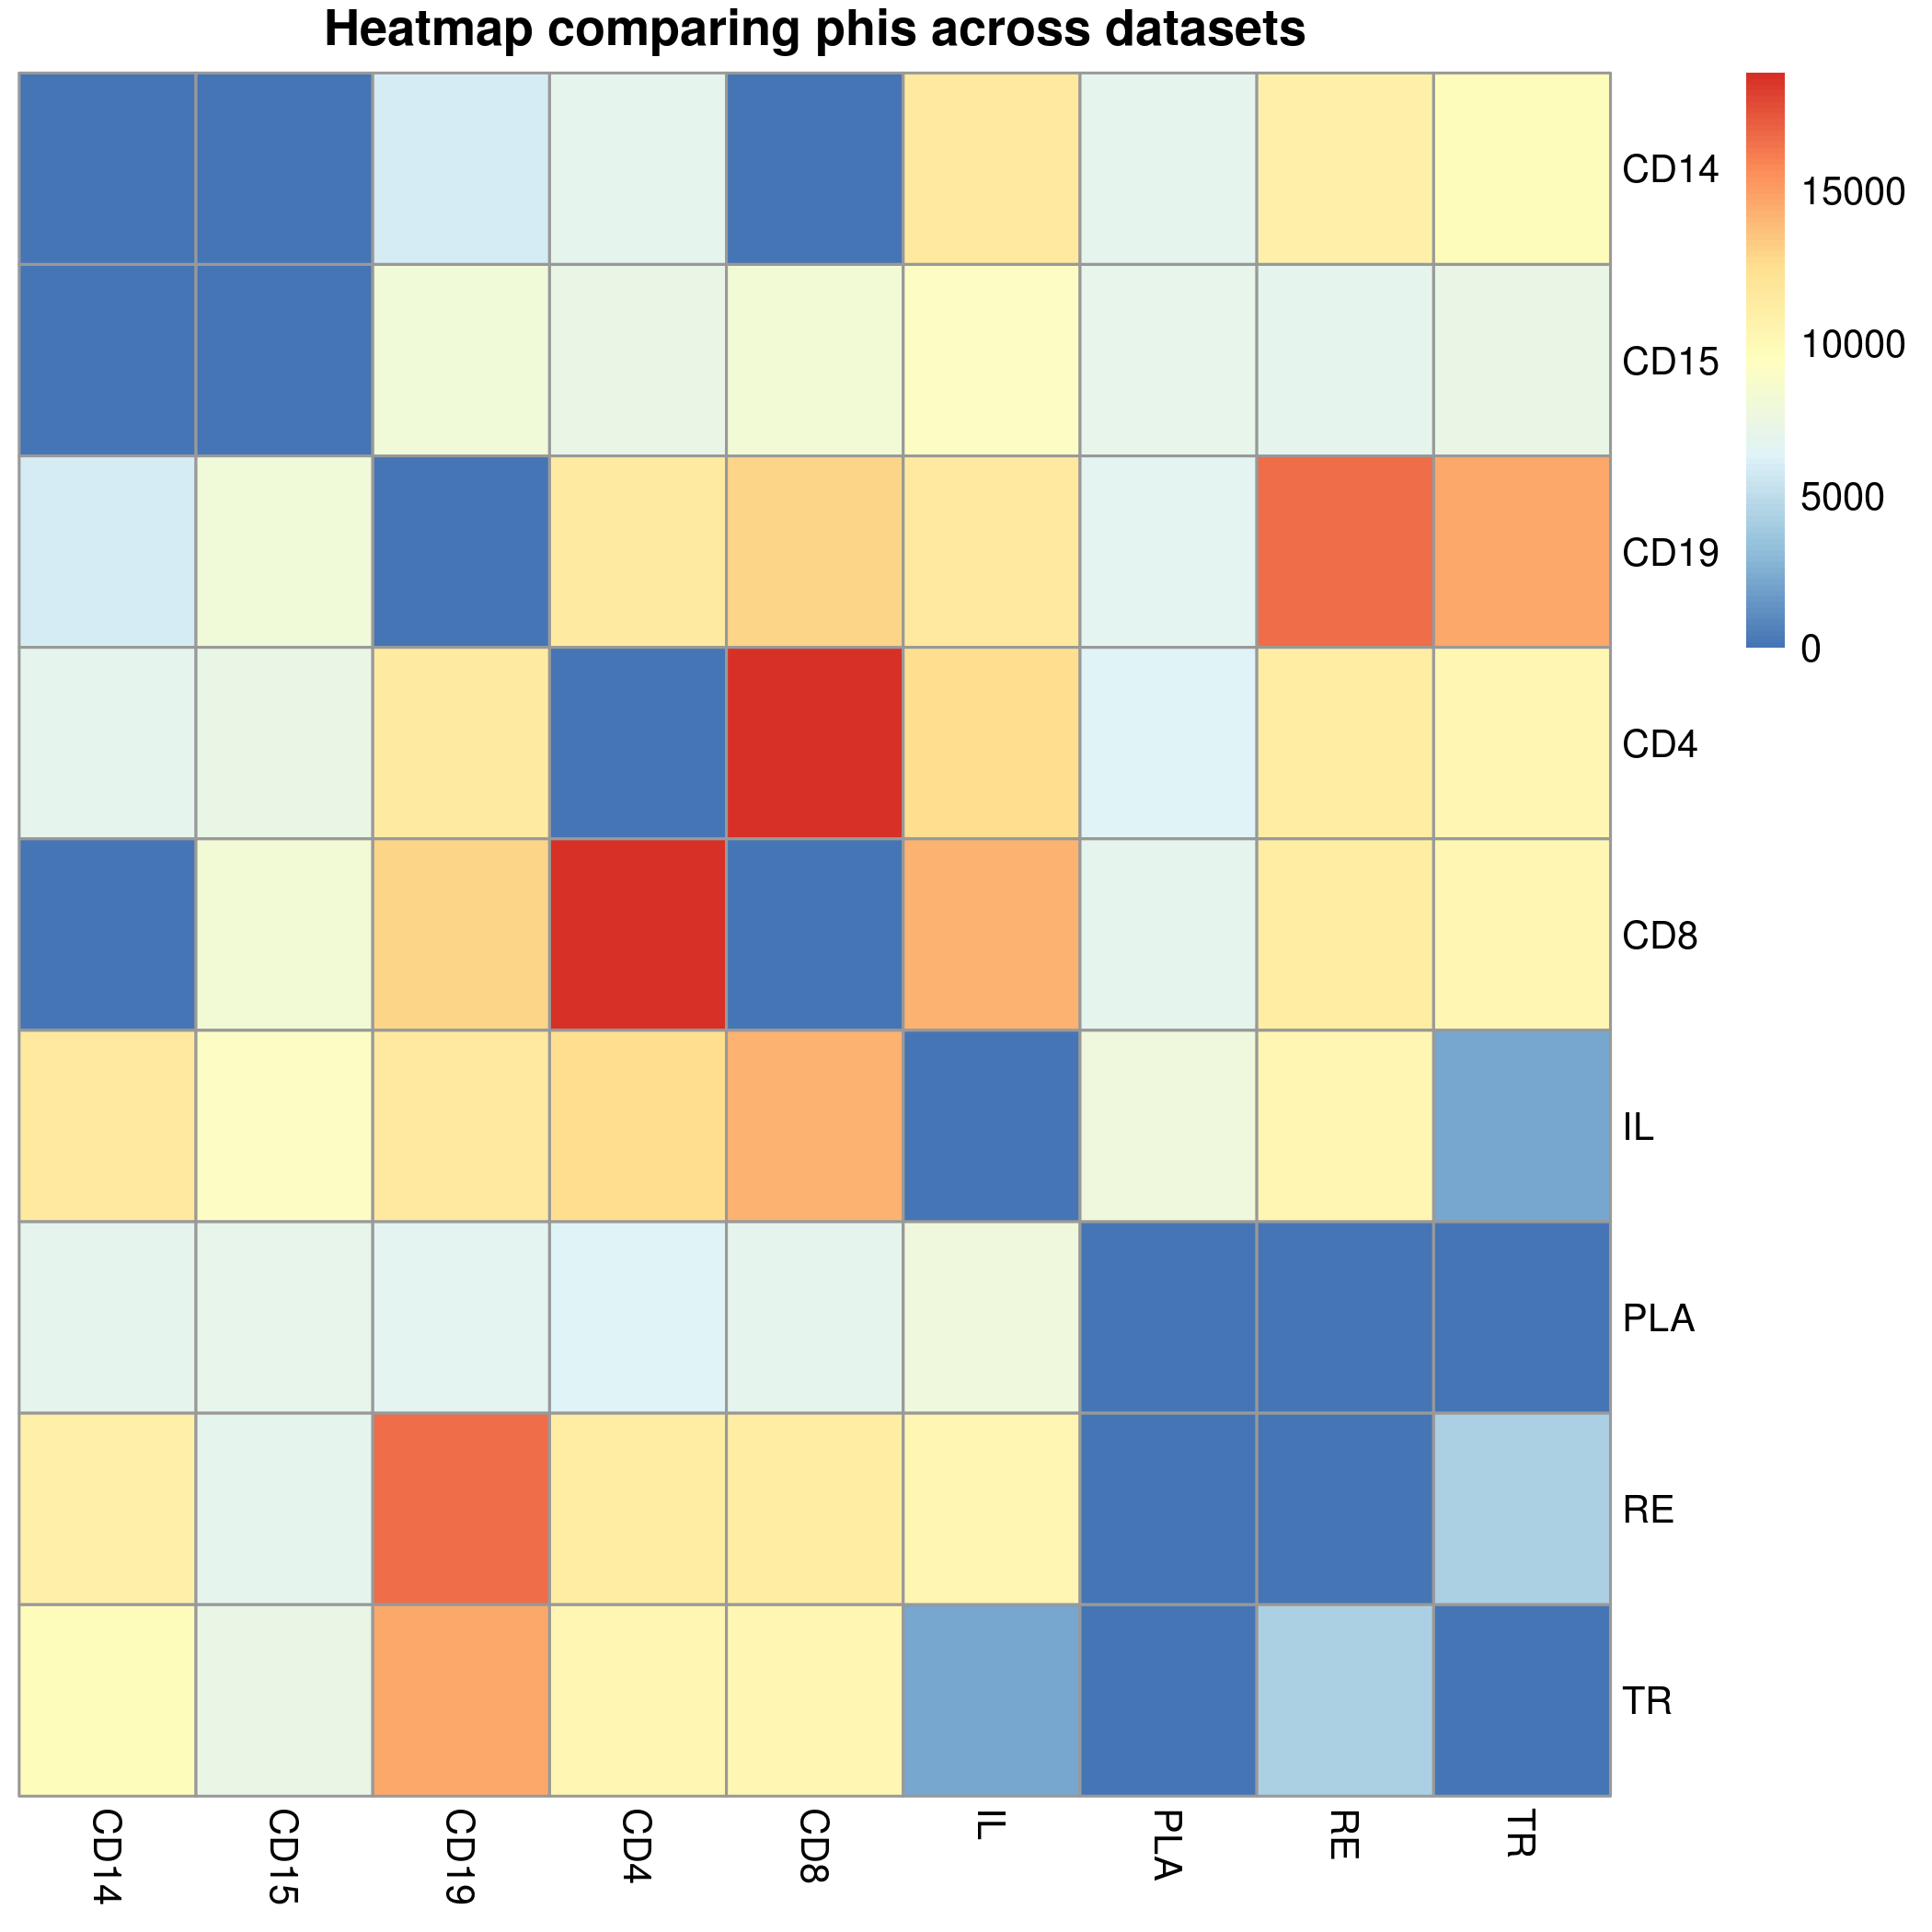
\includegraphics[scale=0.75]{Images/Initial_analysis/Phi_heatmap_1.png}
%		\caption{Mean $\phi$ value between datasets across iterations. $\phi$ can be considered a measure of similarity between datasets - the greater $\phi_{i,j}$ is, the more correlated the clustering in datasets $i$ and $j$ is.}
%		\label{fig:naive_mdi_reduced_phi_heatmap}
%	\end{figure}
%	
%	However, there is too much information in figure \ref{fig:naive_mdi_reduced} for serious analysis and we must use subsets of the data to better understand the information contained here. Based on the clusters of datasets mentioned in \label{list:datasets_naive_mdi_reduced}, we visualise the clustering in these groups.
%	
%	From figures \ref{fig:naive_mdi_reduced_il_tr_cluster} and \ref{fig:naive_mdi_reduced_cd14_cd4_cd8_cluster}, one can see that inspecting the clusters in subsets of the datasets makes it easier to see similarity in clustering.
%	
%	
%%	\begin{figure}[h]
%%		%	\centering
%%		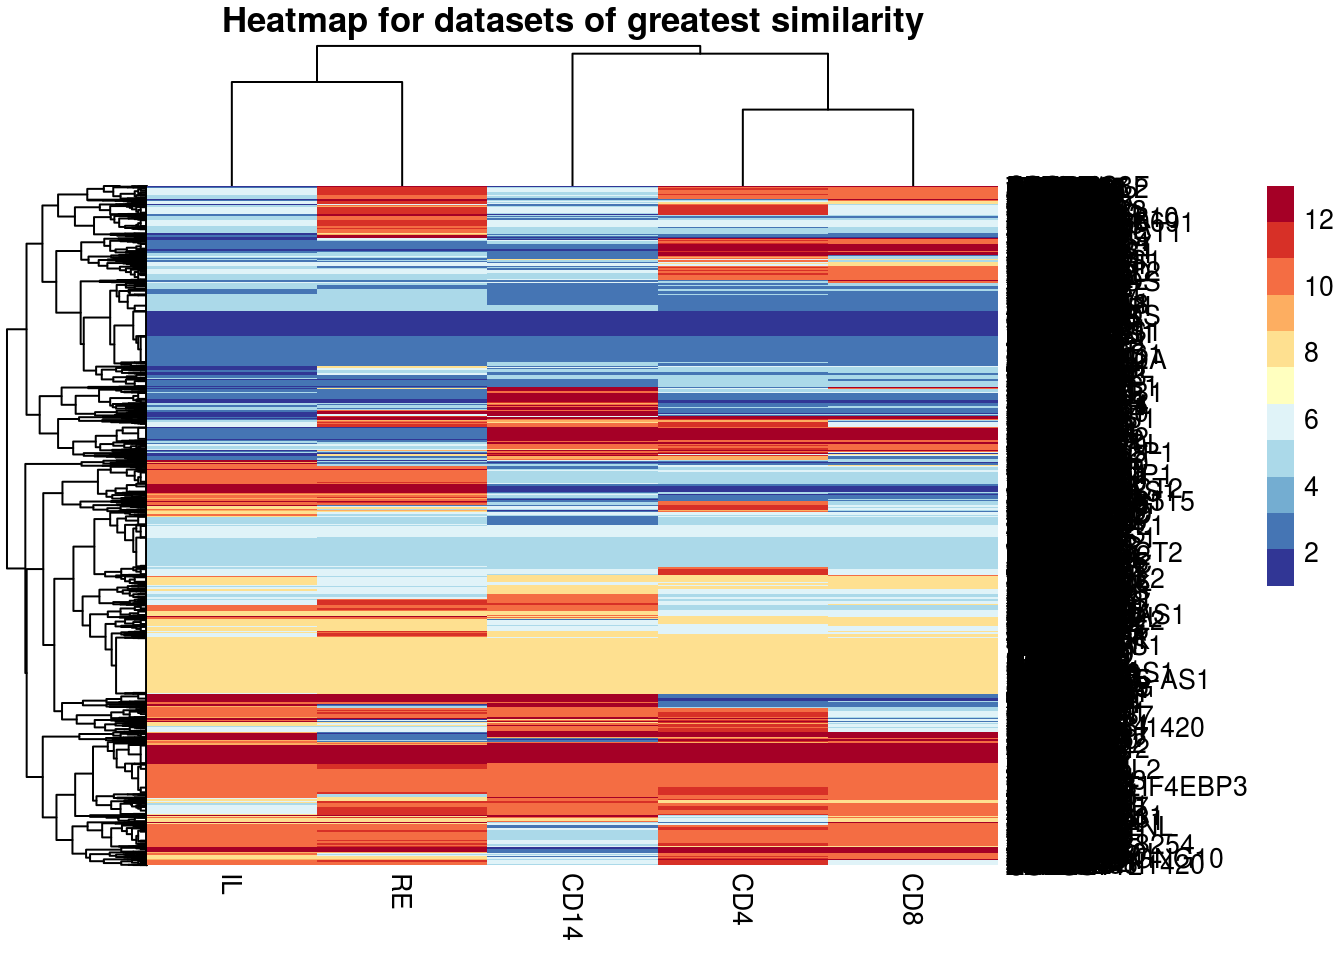
\includegraphics[scale=1.0]{Images/Initial_analysis/sim_heatmaps-1.png}
%%		\caption{Predicted clusters for MDI applied to 9 datasets for common probes with datasets as columns and probes as rows.}
%%		\label{fig:naive_mdi_reduced}
%%	\end{figure}
%
%	\begin{figure}[h]
%		%	\centering
%		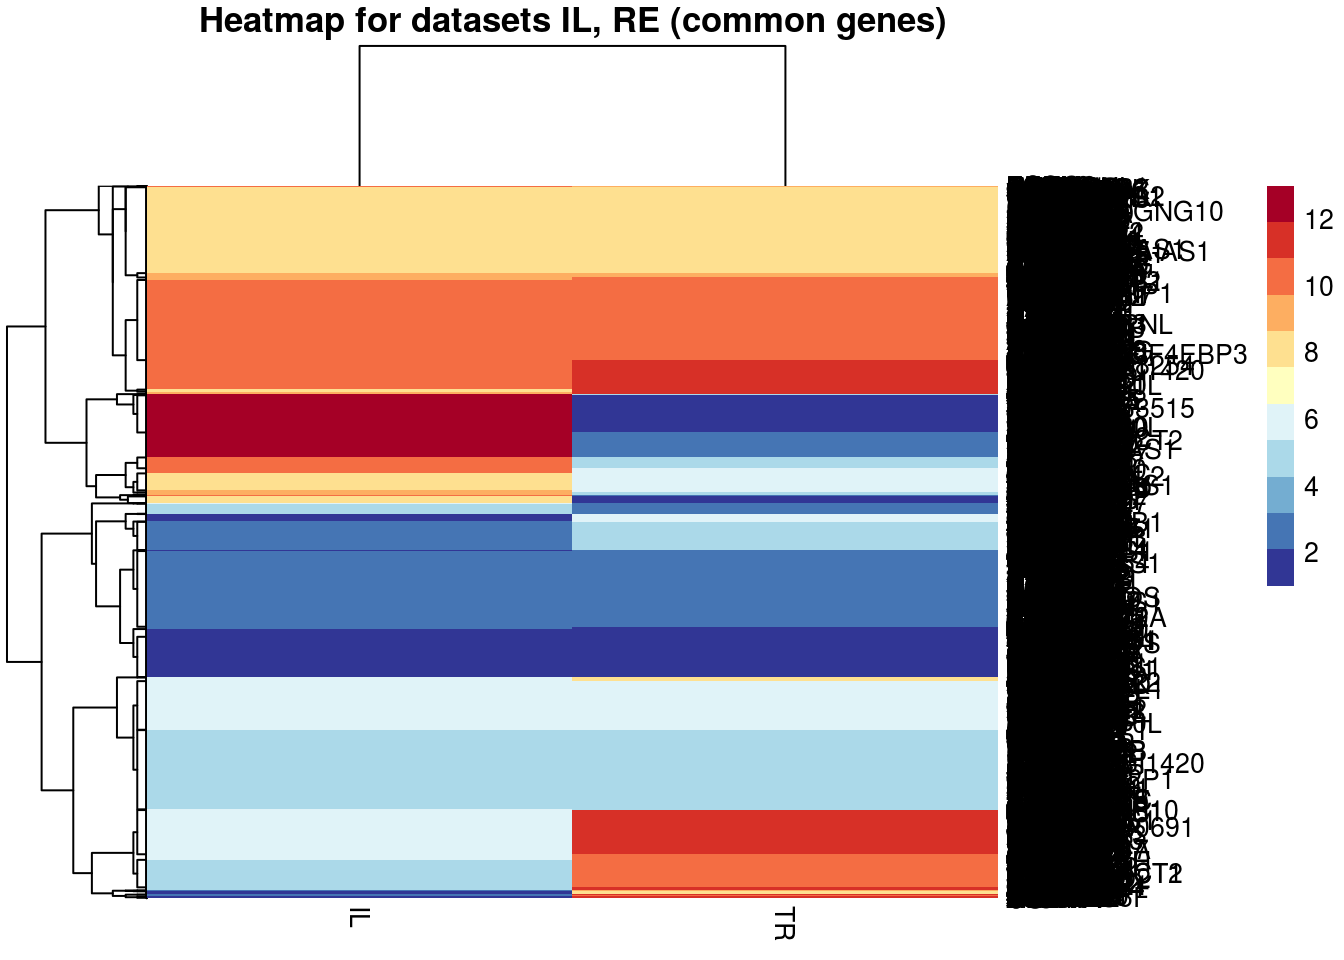
\includegraphics[scale=1.0]{Images/Initial_analysis/sim_heatmaps-2.png}
%		\caption{Predicted clusters for MDI applied to 9 datasets for common probes with datasets as columns and probes as rows.}
%		\label{fig:naive_mdi_reduced_il_tr_cluster}
%	\end{figure}
%	
%	\begin{figure}[h]
%		%	\centering
%		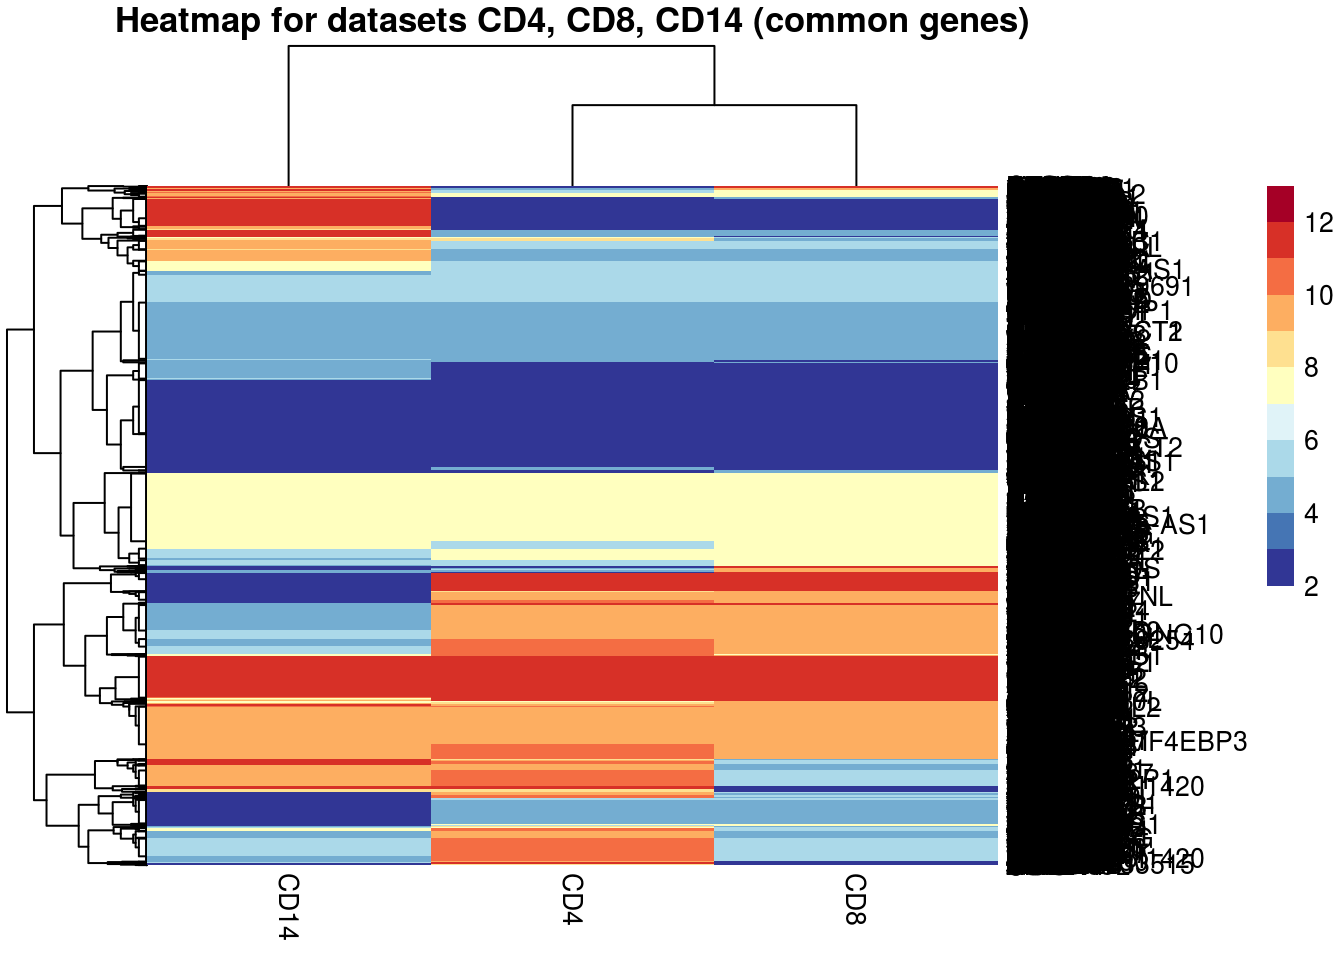
\includegraphics[scale=1.0]{Images/Initial_analysis/sim_heatmaps-3.png}
%		\caption{Predicted clusters for MDI applied to 9 datasets for common probes with datasets as columns and probes as rows.}
%		\label{fig:naive_mdi_reduced_cd14_cd4_cd8_cluster}
%	\end{figure}
%
%	\begin{figure}[h]
%	%	\centering
%	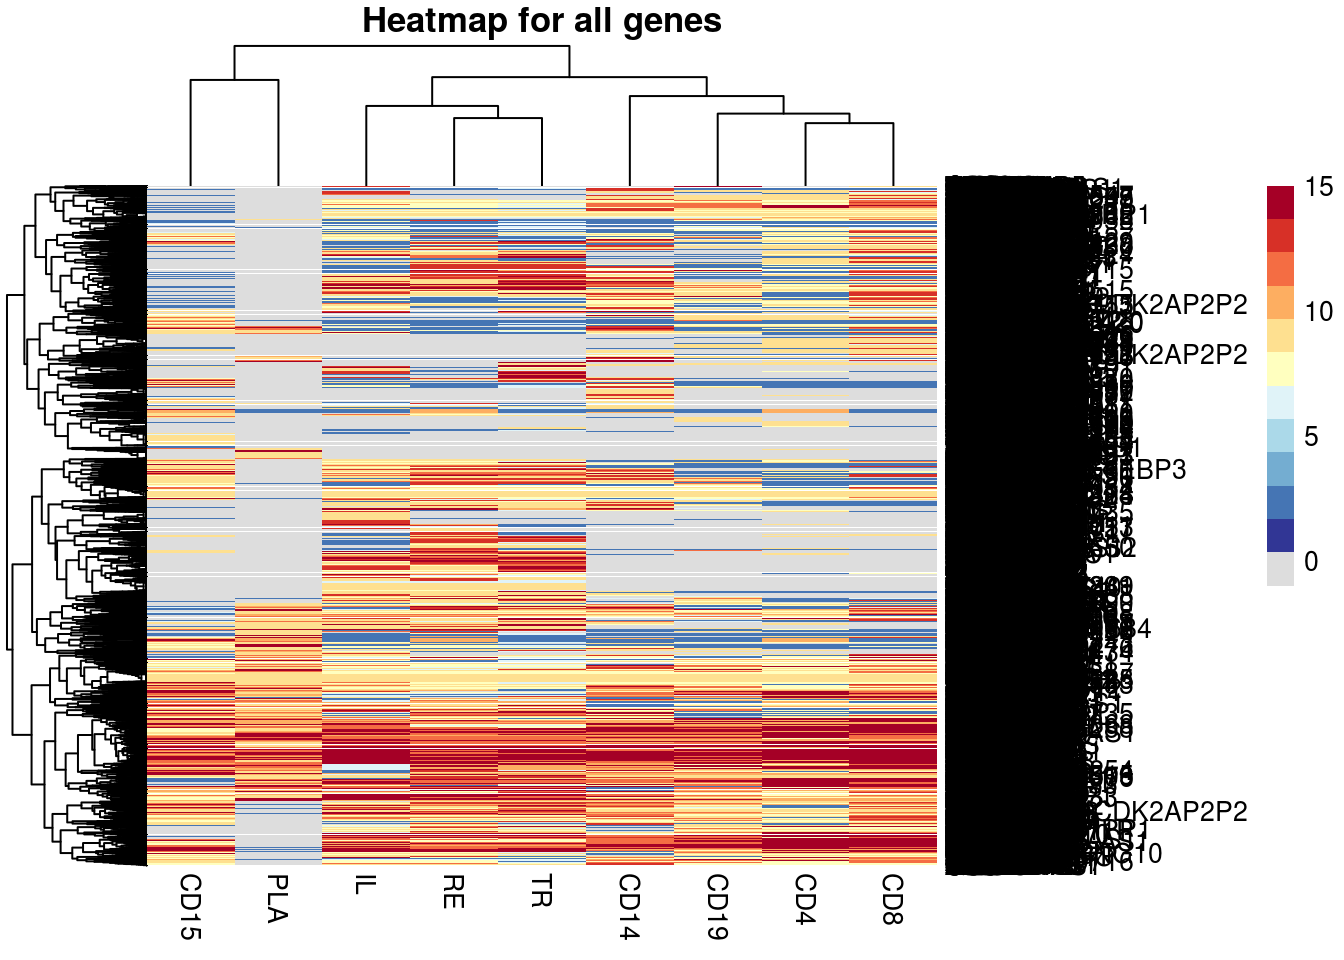
\includegraphics[scale=1.0]{Images/Initial_analysis/mdi_2_heatmap-1.png}
%	\caption{Predicted clusters for MDI applied to 9 datasets for all probes.}
%	\label{fig:naive_mdi_full}
%\end{figure}
	
	\newpage



	%\bibliographystyle{abbrv}
	\bibliographystyle{plainnat}
%	\bibliography{thesis}
	\bibliography{thesis_ref_better}
	

\newpage

\appendix
\section{Data generation explained}

\section{Additional convergence plots}
\subsection{Case 1: Convergence diagnostics}

\subsubsection{Geweke plots}

\subsubsection{Estimated burn in}
\begin{figure}[h]
	\centering
	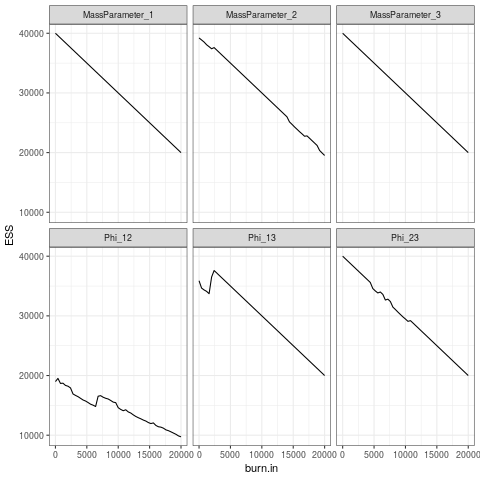
\includegraphics[scale=0.65]{Images/Gen_data/Case_1/Esimated_burn_in_plot_1.png}
	\caption{Box plots for distribution of adjusted rand index between the clustering at each iteration to the true clustering for different lengths of consensus clustering and the collapsed long chains.}
	\label{fig:case_1_esimated_burn_in_plot_1}
\end{figure}

\begin{figure}[h]
	\centering
	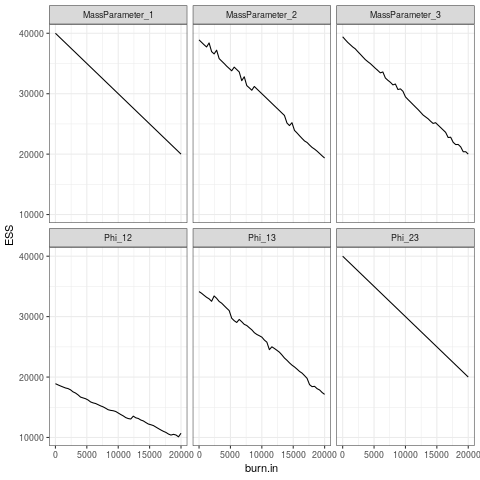
\includegraphics[scale=0.65]{Images/Gen_data/Case_1/Esimated_burn_in_plot_2.png}
	\caption{Box plots for distribution of adjusted rand index between the clustering at each iteration to the true clustering for different lengths of consensus clustering and the collapsed long chains.}
	\label{fig:case_1_esimated_burn_in_plot_2}
\end{figure}

\begin{figure}[h]
	\centering
	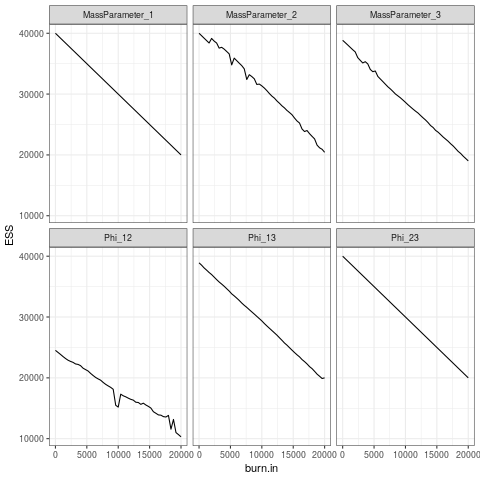
\includegraphics[scale=0.65]{Images/Gen_data/Case_1/Esimated_burn_in_plot_3.png}
	\caption{Box plots for distribution of adjusted rand index between the clustering at each iteration to the true clustering for different lengths of consensus clustering and the collapsed long chains.}
	\label{fig:case_1_esimated_burn_in_plot_3}
\end{figure}

\begin{figure}[h]
	\centering
	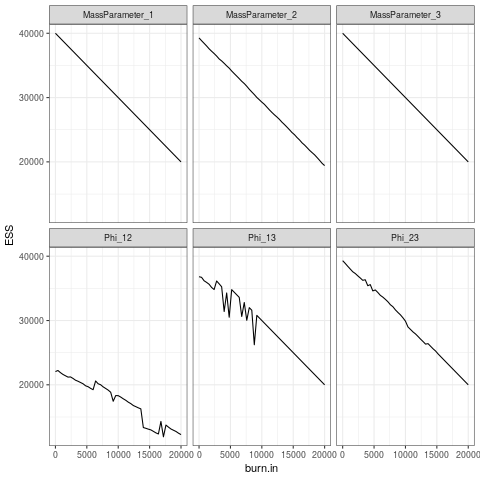
\includegraphics[scale=0.65]{Images/Gen_data/Case_1/Esimated_burn_in_plot_4.png}
	\caption{Box plots for distribution of adjusted rand index between the clustering at each iteration to the true clustering for different lengths of consensus clustering and the collapsed long chains.}
	\label{fig:case_1_esimated_burn_in_plot_4}
\end{figure}

\begin{figure}[h]
	\centering
	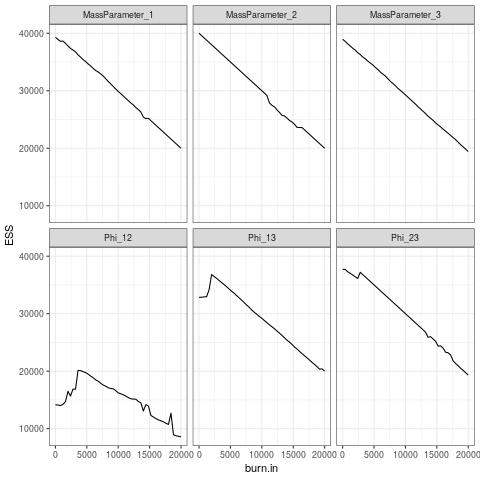
\includegraphics[scale=0.65]{Images/Gen_data/Case_1/Esimated_burn_in_plot_5.png}
	\caption{Box plots for distribution of adjusted rand index between the clustering at each iteration to the true clustering for different lengths of consensus clustering and the collapsed long chains.}
	\label{fig:case_1_esimated_burn_in_plot_5}
\end{figure}

\begin{figure}[h]
	\centering
	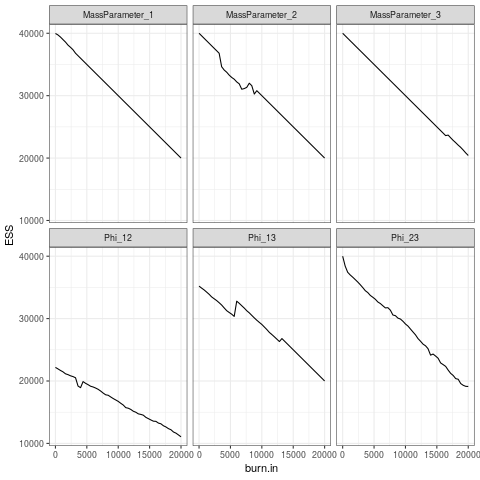
\includegraphics[scale=0.65]{Images/Gen_data/Case_1/Esimated_burn_in_plot_6.png}
	\caption{Box plots for distribution of adjusted rand index between the clustering at each iteration to the true clustering for different lengths of consensus clustering and the collapsed long chains.}
	\label{fig:case_1_esimated_burn_in_plot_6}
\end{figure}

\begin{figure}[h]
	\centering
	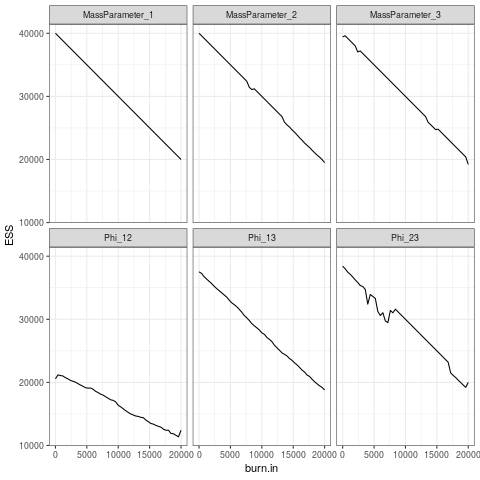
\includegraphics[scale=0.65]{Images/Gen_data/Case_1/Esimated_burn_in_plot_7.png}
	\caption{Box plots for distribution of adjusted rand index between the clustering at each iteration to the true clustering for different lengths of consensus clustering and the collapsed long chains.}
	\label{fig:case_1_esimated_burn_in_plot_7}
\end{figure}

\begin{figure}[h]
	\centering
	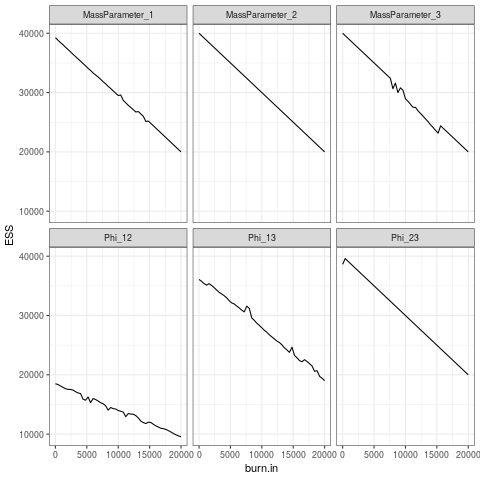
\includegraphics[scale=0.65]{Images/Gen_data/Case_1/Esimated_burn_in_plot_8.png}
	\caption{Box plots for distribution of adjusted rand index between the clustering at each iteration to the true clustering for different lengths of consensus clustering and the collapsed long chains.}
	\label{fig:case_1_esimated_burn_in_plot_8}
\end{figure}

\begin{figure}[h]
	\centering
	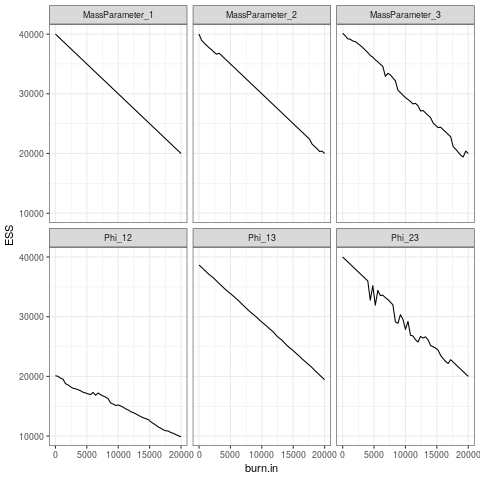
\includegraphics[scale=0.65]{Images/Gen_data/Case_1/Esimated_burn_in_plot_9.png}
	\caption{Box plots for distribution of adjusted rand index between the clustering at each iteration to the true clustering for different lengths of consensus clustering and the collapsed long chains.}
	\label{fig:case_1_esimated_burn_in_plot_9}
\end{figure}

\begin{figure}[h]
	\centering
	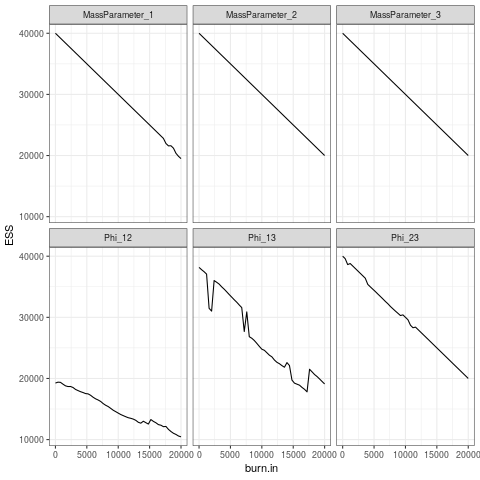
\includegraphics[scale=0.65]{Images/Gen_data/Case_1/Esimated_burn_in_plot_10.png}
	\caption{Box plots for distribution of adjusted rand index between the clustering at each iteration to the true clustering for different lengths of consensus clustering and the collapsed long chains.}
	\label{fig:case_1_esimated_burn_in_plot_10}
\end{figure}





\subsection{Case 2: Convergence diagnostics}

\subsubsection{Geweke plots}

\subsubsection{Estimated burn in}

\begin{figure}[h]
	\centering
	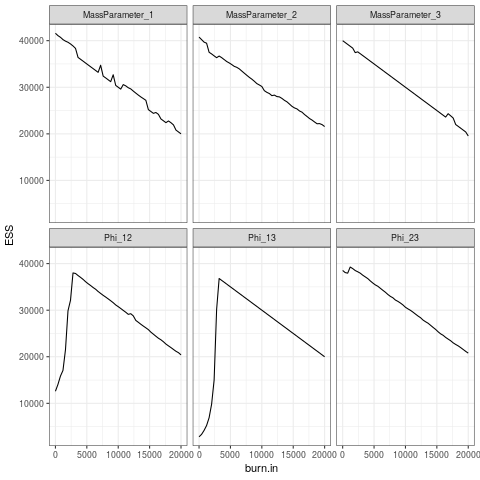
\includegraphics[scale=0.65]{Images/Gen_data/Case_2/Esimated_burn_in_plot_1.png}
	\caption{Plot of effective sample size (ESS) to burn-in for chain 1.}
	\label{fig:case_2_esimated_burn_in_plot_1}
\end{figure}

\begin{figure}[h]
	\centering
	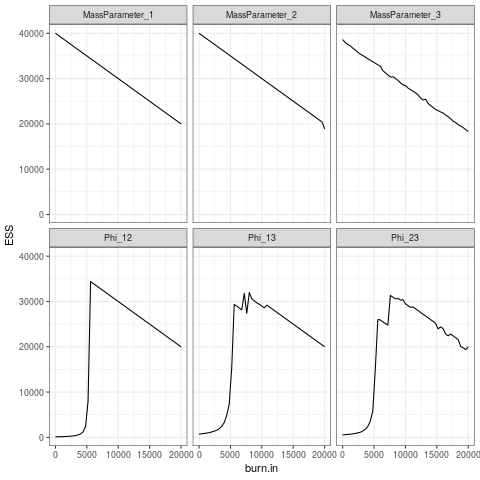
\includegraphics[scale=0.65]{Images/Gen_data/Case_2/Esimated_burn_in_plot_2.png}
	\caption{Plot of effective sample size (ESS) to burn-in for chain 2.}
	\label{fig:case_2_esimated_burn_in_plot_2}
\end{figure}

\begin{figure}[h]
	\centering
	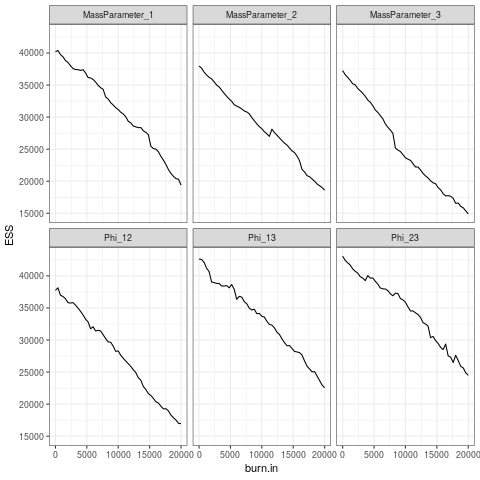
\includegraphics[scale=0.65]{Images/Gen_data/Case_2/Esimated_burn_in_plot_3.png}
	\caption{Plot of effective sample size (ESS) to burn-in for chain 3.}
	\label{fig:case_2_esimated_burn_in_plot_3}
\end{figure}

\begin{figure}[h]
	\centering
	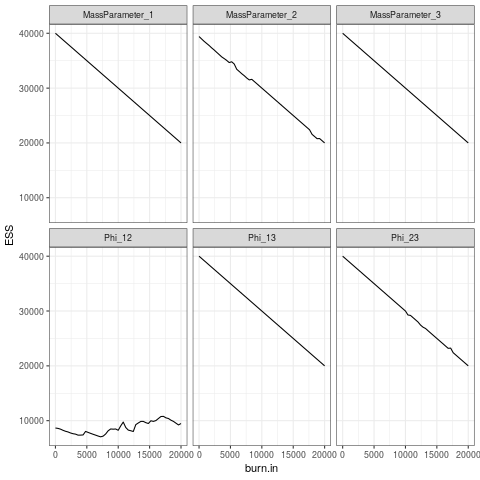
\includegraphics[scale=0.65]{Images/Gen_data/Case_2/Esimated_burn_in_plot_4.png}
	\caption{Plot of effective sample size (ESS) to burn-in for chain 4.}
	\label{fig:case_2_esimated_burn_in_plot_4}
\end{figure}

\begin{figure}[h]
	\centering
	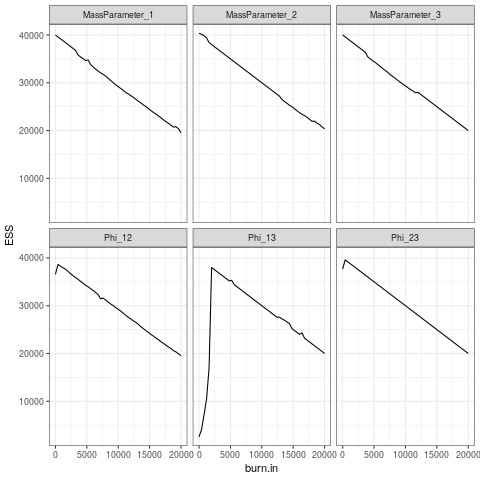
\includegraphics[scale=0.65]{Images/Gen_data/Case_2/Esimated_burn_in_plot_5.png}
	\caption{Plot of effective sample size (ESS) to burn-in for chain 5.}
	\label{fig:case_2_esimated_burn_in_plot_5}
\end{figure}

\begin{figure}[h]
	\centering
	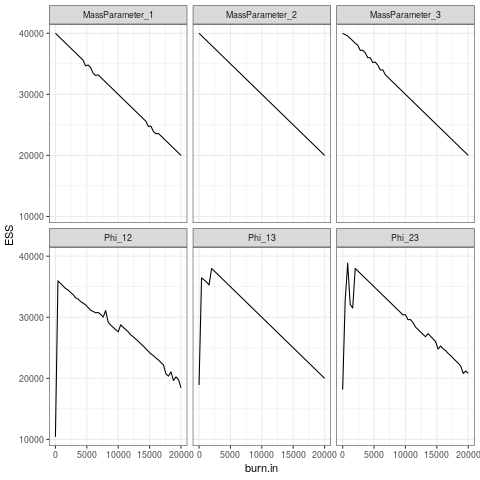
\includegraphics[scale=0.65]{Images/Gen_data/Case_2/Esimated_burn_in_plot_6.png}
	\caption{Plot of effective sample size (ESS) to burn-in for chain 6.}
	\label{fig:case_2_esimated_burn_in_plot_6}
\end{figure}

\begin{figure}[h]
	\centering
	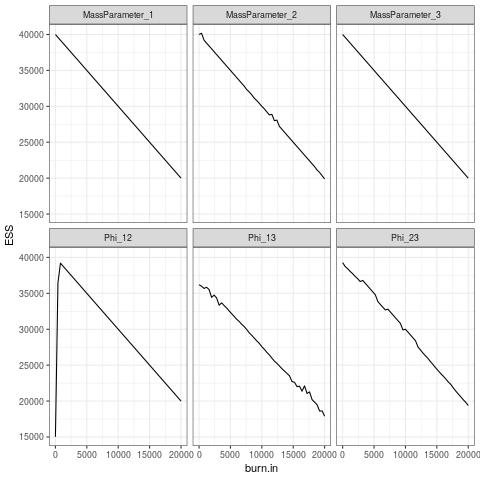
\includegraphics[scale=0.65]{Images/Gen_data/Case_2/Esimated_burn_in_plot_7.png}
	\caption{Plot of effective sample size (ESS) to burn-in for chain 7.}
	\label{fig:case_2_esimated_burn_in_plot_7}
\end{figure}

\begin{figure}[h]
	\centering
	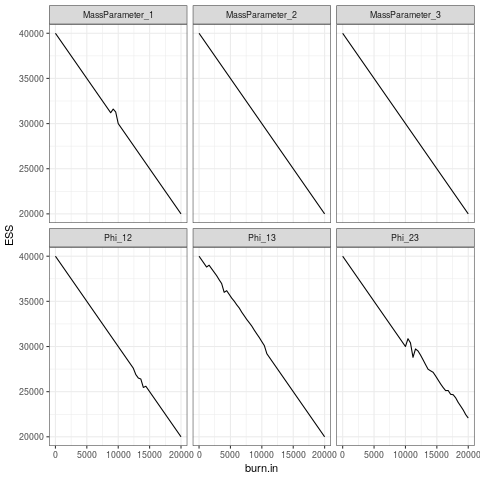
\includegraphics[scale=0.65]{Images/Gen_data/Case_2/Esimated_burn_in_plot_8.png}
	\caption{Plot of effective sample size (ESS) to burn-in for chain 8.}
	\label{fig:case_2_esimated_burn_in_plot_8}
\end{figure}

\begin{figure}[h]
	\centering
	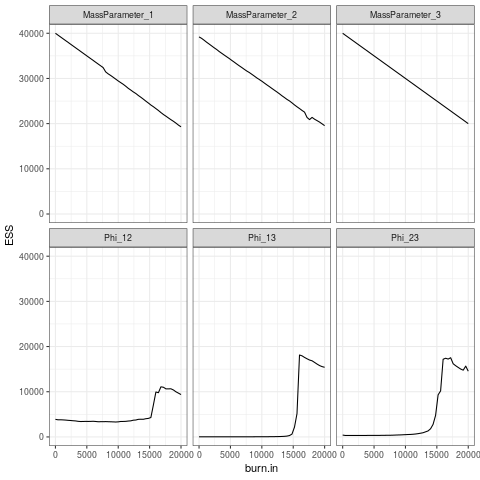
\includegraphics[scale=0.65]{Images/Gen_data/Case_2/Esimated_burn_in_plot_9.png}
	\caption{Plot of effective sample size (ESS) to burn-in for chain 9.}
	\label{fig:case_2_esimated_burn_in_plot_9}
\end{figure}

\begin{figure}[h]
	\centering
	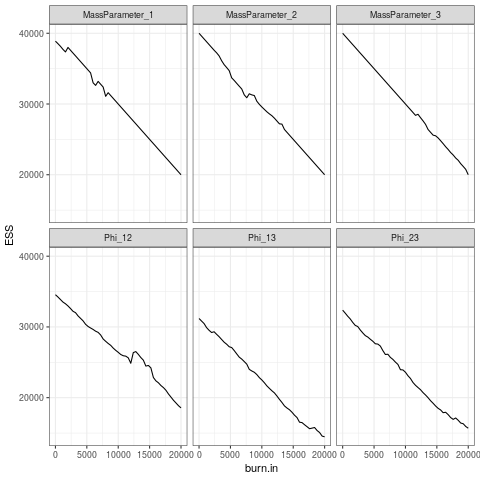
\includegraphics[scale=0.65]{Images/Gen_data/Case_2/Esimated_burn_in_plot_10.png}
	\caption{Plot of effective sample size (ESS) to burn-in for chain 10.}
	\label{fig:case_2_esimated_burn_in_plot_10}
\end{figure}

\end{document}